\documentclass[a4paper,12pt]{report}
\usepackage[T1]{fontenc} 
\usepackage[utf8]{inputenc}
\usepackage{subfig}
\usepackage{graphicx}
\graphicspath{ {./images/} }
\usepackage{epstopdf}
\usepackage{amsmath}
\usepackage{amsfonts}
\usepackage{amsthm}
\usepackage{array}
\usepackage{bm}
\usepackage{amssymb}
\usepackage{esvect}
\usepackage{caption}
\usepackage{cite}
%\usepackage{subcaption}
\usepackage{epstopdf}
\usepackage{fancyhdr} 
\usepackage{fullpage}
\usepackage{eso-pic} 
\usepackage[english]{babel}
\usepackage{rotating}
\usepackage{tikz}
\usepackage{float}
\usepackage{rotfloat}
\usepackage[titletoc]{appendix}
\usepackage{booktabs}
\usepackage{multicol}
\usepackage{multirow}
\usepackage{lscape}
\usepackage{hyperref}
%\usepackage[numbers]{natbib}
\usepackage{titlesec}
\usepackage{url}
\usepackage{colortbl}
	\definecolor{maroon}{rgb}{0.75, 0.75, 0.75}
%\setlength\parindent{10pt}
\setlength{\parindent}{5ex}
%\setlength{\parindent}{4em}
\setlength{\parskip}{0.5em}
%\setlength{\parskip}{1.5pt}
\usepackage[export]{adjustbox}
\usepackage{wrapfig}
\usepackage{gensymb}
\usepackage[official]{eurosym}
\usepackage[nice]{units}
\usepackage{changepage}
\usepackage{pdfpages}
\usepackage{titlepic}
\usepackage{listings}
\usepackage{xcolor}
\usepackage{soul}
\usepackage{breqn}
%\usepackage[prefix,intoc]{nomencl}
%\usepackage[nottoc]{tocbibind}
\RequirePackage{ifthen}
\usepackage{listings}
%\usepackage{tocloft}
\usepackage[framed,numbered]{matlab-prettifier}

\lstset{
  style      = Matlab-editor,
  basicstyle = \fontfamily{pcr}\selectfont\footnotesize, % if you want to use Courier
}

%\usepackage{nomencl}
\usepackage[intoc, english]{nomencl}
\makenomenclature
%% SET types either acronym or symbol FORMAT1 for more references check https://www.overleaf.com/learn/latex/Nomenclatures
\RequirePackage{ifthen}
\renewcommand{\nomgroup}[1]{%
\ifthenelse{\equal{#1}{S}}{\item[\textbf{Symbols}]}{
\ifthenelse{\equal{#1}{A}}{\item[\textbf{Abbreviations}]}{}}}
%%%%

%% Form 2 to set the list of abbreviations and symbols
%\usepackage{etoolbox}
%\renewcommand\nomgroup[1]{%
%  \item[\bfseries
%  \ifstrequal{#1}{S}{Symbols}{%
%  \ifstrequal{#1}{A}{Acronyms}{%
%  \ifstrequal{#1}{C}{Other Symbols}{}}}%
%]}

% ADD GLOSSARIES 
%https://www.overleaf.com/learn/latex/Glossaries
\usepackage[acronym]{glossaries}
\makeglossaries
\newacronym{sname}{SNAME}{Society of Naval Architects and Marine Engineers}
\newacronym{dsyhs}{DSYHS}{Delft Systematic Yacht Hull Series}

\newacronym{b_aw}{$\beta_{aw}$}{Apparent wind angle}
\newacronym{vpp}{VPP}{Velocity Prediction Program/Polar}
\newacronym{nwp}{NWP}{Numerical Weather prediction}
\newacronym{wrf}{WRF}{Weather Research and Forecasting model}

\newacronym{ce}{CE}{Center of Effort}
\newacronym{u}{\textit{u}}{Velocity along the X-axis}
\newacronym{v}{\textit{v}}{Velocity along the Y-axis}
\newacronym{v_tw}{$V_{tw}$}{True Wind Velocity}
\newacronym{b_tw}{$\beta_{tw}$}{True Wind Angle}
\newacronym{kappa}{$\kappa$}{Exponent for wind velocity at different height [1/7,1/4] }

\newacronym{matlab}{$ MATLAB\textsuperscript {\textregistered}$}{MATLAB R2018b Student License}

\newacronym{v_aw}{$V_{aw}$}{Apparent Wind Velocity}
\newacronym{v_tc}{$V_{tc}$}{True Current Velocity}
\newacronym{b_tc}{$\beta_{tc}$}{True Current Angle}
\newacronym{v_awc}{$V_{a_{w,c}}$}{Apparent Velocity due to wind and current}
\newacronym{v_btw}{$V_{tw}^b$}{True Wind Velocity respect to the sailboat}
\newacronym{RM}{$\mathcal{R}$}{Rotational Matrix}
%% List of equations
%\usepackage{tocloft}


% Subtract 1 from counters that are used
\renewcommand{\thesection}{\thechapter.\number\numexpr\value{section}\relax}
\renewcommand{\thesubsection}{\thesection.\number\numexpr\value{subsection}\relax}
\renewcommand{\thesubsubsection}{\thesubsection.\number\numexpr\value{subsubsection}\relax}
\setcounter{secnumdepth}{3}
\setcounter{chapter}{0}% Not using chapters, but they're used in the counters


\title{Review chapter}
\author{Gabriela Pardo Arteaga 4617630}

\date{\today}

\pagenumbering{roman}

\begin{document}
\maketitle

%
%Say very briefly 1) what the review is about, 2) what the main content is, 3) what the main aim or objectives are, and 4) what the main findings are. End with a strong sentence that highlights the significance of the work presented in the review and any envisioned long-standing contribution to the body of knowledge.



%%%Summary
\chapter*{Abstract}
%Say very briefly 1) what the review is about, 2) what the main content is, 3) what the main aim or objectives are, and 4) what the main findings are. End with a strong sentence that highlights the significance of the work presented in the review and any envisioned long-standing contribution to the body of knowledge.
Olympic sailing is characterize by one-boat design in each class, with its particular rules. %These classes are: one windsurfing board, two keelboats and four variants on the dinghy.
Because improvements on the boat are not allow; the scope for many researches is focus on the athlete, enhancing strength and other motor skills. On each class, the competition stand for many races and days where the configurations of the route and the environmental conditions diverse from each other. The winner is the one with the lowest score. In each race, points are given  and %fand in each race every position gives points; 
the higher position the lower score. Athletes and coaches confront distinctive scenarios for which they take different decisions in order to win. One of these decisions refers to the sailing direction taken at the start line.

During competition, it is the athlete who decide the number maneuvers and the direction of each; specially on the upwind condition, the boat sails against the wind
%Since the sailboat can not displace towards the wind, tacking manoeuvers are perform. This type of path is described as 
in a zig-zag pattern that can be started on the left- or on the right-hand side. %Another condition is dictated when the boat is dis- placed in the same direction as wind. These conditions shows that feasible paths are asymmetrical[Dol12]. 
Because athletes are not allow to get any information or feedback from coaches; the information of how to course the race before competition is crucial. \newline
%As in many race competitions, the winner is the one that first cross the end line. In other words
The fastest path results from a trajectory sailed with a minimal time, independently of its length. Because trajectories are defined by the route to sail, the wind and current fields characteristics as intensity and direction, and the sail angle respect to the wind. The selection of the fastest path requires the discretization of the area cover by the route. If wind and current fields are not constants, they also required the discretization respect to location and time. These process define the granularity of the problem to solve and in consequence the computation time to find a solution. % The area of sail  These two discretizations are  Because of this, the problem can be define as an optimization problem with the objective to miminizes the time of the trajectory to f 
%to with the minimal time, The relevance of the fastest path is because during competition the boat that first cross the end line is the winner which means

The purpose of this study is to model the path for sailing competitions and optimize the minimal time of sailing routes for the Laser (Olympic class) shaped by wind. Furthermore, identify the effects of different time steps on the resulting times and trajectories.
%In other words,%the critical variables influenced by the wind that determine it.
%the study seek 
%To answer the question, What is the optimal sailing route for the Laser (Olympic class) shaped by wind. The objective is to analyze the sensibility of the optimal route due to changes on the wind field and start times. This will determine the zones and the shape trajectory of the optimal path. 
%and conditions that shape not only the optimal but the least route also. 
To answer this question first, the physical model of yachts was reviewed. Despite the similarities between dinghies(Laser boats) and yachts, the physical model was adapted by adding two coefficients related with sails which indicate%the research focusing on dinghies is significantly lower as consequence adaptations have been made to represent
how different is steering a dinghy from a yacht. Moreover, these adaptations are reflected on the %These adaptations are related with the
Velocity Prediction Polar (VPP)diagram. By using the VPP and the wind intensity is possible to set the direction at which the dinghy reach is maximum velocity respect to the wind. This approach is known as Velocity Made Good (VMG).%  and to more specific and the use of sails
%Despite the similarities between dinghies and yachts, the research focusing on dinghies is significantly lower as consequence adaptations have been made to represent how it is steering, one of this is related with the VPP's and the use of sails. The same situation happens when the topic of research is related with optimal routes.  Since Olympic sailing is focused on the seamanship, the understanding of physical principals intends to provide or reveal hints that helps them to train and contest effectively regardless the location and routes. \newline

%The report answers the question of what device should be developed 
%%most be included on a portable device% 
%for people without impaired limbs; such as the ageing,  to enhance the motion of the upper limb in terms of force and what are the most (technically) feasible features to include on it to improve the life quality of the users.% %design that enhances the human force of the upper limb. 
%To answers these questions first  
%%This will be done by means of the 
%a literature study about the topic was done. Then, an inventory analysis was developed about the devices available on the market that enhance force. From this analysis,  the requirements and the critical features were identified and three concepts were developed. %the .% 
%This report asses them 
%%these portable designs %the three concepts  
%with the multi-criteria analysis method to identify the most feasible design to enhance the force of the upper limb for people without impaired limbs. The design %with the higher score 
%obtained from the assessment was the powered exoskeleton with monitoring system.
The algorithm developed is limited to dinghies which is one of the Olympic boat classes and the smallest; and it was validated by comparing its results against the results of previous races located at Hyères, France during 2018. Three wind conditions were tested, first is was assume that the wind intensity and direction are constant along the area of the route; the second, considers a forecast wind field as time-space-dependent variable changing every 10 minutes without current and neglecting the wave disturbances and twisting effects on the sail, the last test condition uses the wind measurements took during the competition. 

The preliminary tests show that results are closer when the wind is assuming constant and when VPP used is estimating from the top 10 competitors of the competition. The dynamic model of the dinghy requires further research to give more predictable and accurate results. Olympic Classes as dinghy is not a widespread research topic. Besides most of the findings related to path optimization for boats are related with cargo ships and vessels, where the main objective is to minimize the fuel costs, because these ship can be set to navigate at a constant speed. The influence of the wind is not the same as for the Olympic Classes. Another consideration that should be taken is related with the movement of the sailor which affect the equilibrium of the boat and therefore the maximum speed that could be reach.  %The reason for this is that limited data was available, as sailboat modelling is not a widespread
 %Also, on formulating a sailing trajectory optimization as an optimal control problem, very limited information was available.
%Although quite some problems have been solved, the results can be improved by future re- search, by addressing the most important recommendations below.
%Towing tank, open water and wind tunnel tests could be carried out to determine the hy- drodynamic and aerodynamic characteristics of the dinghies, to be able to incorporate higher order dynamics into the model over a wider range of boat and wind speeds.
%In this thesis the focus was on determining the advantage in an upwind leg of the route based on currents, but a more detailed model could also help in the future to optimize and analyse the trimming of the sail, rudder action or even the movement of the sailor.
%Furthermore, the focus was on the influence of currents, but in the results some cases subject to wind variations were treated. In future research wind dynamics could be implemented much more detailed. For this, a proper wind model should be developed. But this would need specific attention because wind is much more subject to uncertainties than currents.
%Furthermore, other boat types, multiple competitors and weather uncertainties could be im- plemented in future research.

The report is set as follows: Chapter 1 refers to the basics concepts of sailboat and wind fields, Chapter 2 describes the mathematical model for sailboat in general and the modifications required. The validation of the model is reviewed on chapter 3. In Chapter 4 the obtained results are analyzed and finally the conclusions and recommendations are described in Chapter 5.\par 
%\addcontentsline{toc}{chapter}{List of Symbols}
%\chapter*{List of Symbols}
\renewcommand{\nomname}{List of Symbols}\label{list:symbols}
\renewcommand{\nompreamble}{The next list describes several symbols that will be later used within the body of the document}
\printnomenclature

\newpage

\renewcommand*\contentsname{Summary}

\tableofcontents
%\addcontentsline{toc}{chapter}{}{}

%\restoretocpage
\newpage
\pagenumbering{arabic}
\setcounter{page}{1}


\chapter{Introduction}

%Introduce the general area of interest that the contents of the review deal with, setting out any advancements and challenges of interest. Then introduce more fully the specific topic addressed in the review and you can then to go on to state any main aim or objectives to be met. Say very briefly what is to come in the layout of the review. Note: the Introduction should include general references to back up the points made.
% Establishing the field
%Definition:
%What are the Olympic classes sailing?
%How are the competitions setting  up?
%What does position and direction means?
%What time steps are you referring for the wind forecast, which sizes?

%Add significance of the main question be sure this was explained properly 
In recent years the integration of new technologies on training programs of professional athletes have been increased. Not only to enhance their motor skills, and to prevent injuries but also to obtain better results with minimal time and in a more efficient process. For example, the use of information that specifies the conditions or parameters that deliver the best results to win, have gained more popularity within the sports community. The involvement of science like kinesiology \cite{sjogaard2015science}, movement science; and engineering is not only concentrated in the athletes but in the elements and factors that cannot be controlled by them, but by those that impact their results. One of these sports is sailing where athletes have to guide the sailboat under different weather conditions and where time is crucial to winning the race.\par
During sailing races such as coastal, inland waterways and lakes, athletes are not allowed to get any information from coaches during the race; for this reason, their preparation and training are not only physical. During training, they acquire skills to anticipate the weather changes and at the same time maneuvers to improve the performance of the sailboat. \par
%For example, a well know competition and classes are the Olympic sailing competitions which take place on coastal and improvements on the boat are not allow. \\
In this section, the research problem, its relevance, and the objectives are going to be presented. For this, a brief definition of Olympic sailing classes and courses are going to be explained followed by an explanation of the information considered by the coaches and athletes to plan the strategy before the competition takes place which most of the time refers to the weather forecast. These data provide a framework to set-up the assumptions and limitations considered in this research. \par 
\section {Olympic Sailing} \label{sec:olympic classes}
The Olympic Sailing Classes are characterized by the rule of a one-design boat. Each class is defined by the sailboat to use; type, size of the hull, number of sails, area, and style, the size of the crew and the gender of them.  The intention of this is to leave out the influence of technology on the results and to focus on the abilities of the athlete to perform effectively; for this reason, the scope for many types researches is on the athlete only. Figure \ref{fig:olymp_cla} shows the names and categories of the current classes that the International Federation of sailing defines as Olympic Classes. The list is subject to change and it is reviewed every 4 years when the Olympic Games have been completed.\par 
The dinghy is not only the smallest and simplest sailboat, one sail and one hull, propelled by wind, but the one used in most of the classes. The differences between their classes rely on the dimensions of the boat and sail, despite using the same type of boat, these differences impact on the speed of the boat and maneuverability. The dimensions on the hull and sails are determined by the number of crew members,1 or 2, and their gender. This research is going to use the dinghy as a reference boat; because is the simple boat, one hull one sail, used extensively on the Olympic Classes. Another reason is due to its similarity physically and mathematically with yachts which have been studied since 1979 \cite{marchajaereo1979}, this allows that some approaches and information can be taken or borrow from them, either to compare or validate the results obtained.\par 

\begin{figure}[ht]
\centering
 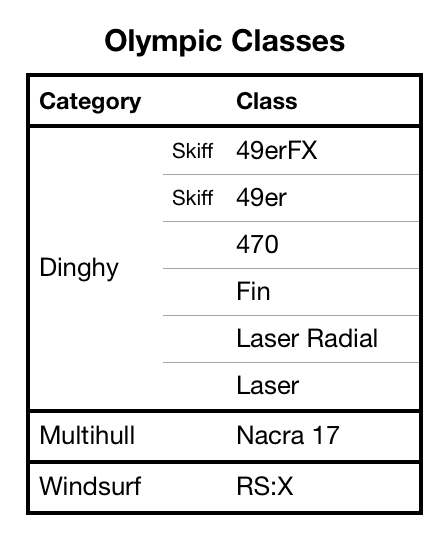
\includegraphics[width=0.32\textwidth]{olym_classes.png}
  \caption{Olympic classes \cite{sailoly}.}
\label{fig:olymp_cla} 
\end{figure}

The competition in each class stands for many races and days where the configurations of the course vary according to the environmental conditions. In each race, points are given according to its arrival position; the faster, the lower the score. The winner is the one with the lowest score. Under this competing format, athletes and coaches confront distinct scenarios for which they take different decisions at the starting line. One of these decisions refers to the initial sailing direction. Its importance is related to the configuration of the course.\par 

\section{Competition Course}\label{tracks}
The most common form of a sailing competition is the fleet racing where all participants race around a course and start at the same time along with a line. Here, not only is the reaction time important but the direction that allows the maximum speed that could be attained is too. Usually, two different types of courses take place in the Olympic classes. Figure \ref{fig:trap_c} shows the singular trapezoid course which is defined by a separate start and finish line and 4 points around (buoys); these 6 elements define the legs of the competition, the first leg is usually the longest one and it is running against the wind.
The trapezoid course is the most completed format courses, the other formats are a partial representation of it, considering only some legs which are already represented in the trapezoid course.\par 
%The other course is the windward/leeward, figure \ref{fig:wl_c} this is simply a two-leg race orientated in such way that the first leg is sail against the wind (called a beat) and the second leg is sail with the wind (called a run). If boats are sailing neither with nor against the wind, the leg is called reach. 

The courses characteristics and conditions of race are also subject to change every 4 years. For example, the current course is regulated as follows \cite{race_pol}: The length and angles of each leg are defined in such way that the course could be completed in maximum 1 hour and the trapezoidal course can be contained in a grid size of 2km by 2km.  Another consideration is the area of the course,  which most of the time is expressed in nautical miles (nm).Figure \ref{fig:olymp_areas_rio} is an example of how the sailing areas are defined by a circular area, within this circle the trapezoid should be located. \par 
Furthermore, the wind conditions refer to the average wind speed in addition to its shift direction. The current regulation establishes that the race will not start if the average wind speed is less than 4 knots(kn)[2 m/s] or more than 25 knots(12.86 m/s) over the entire course, with maximum wind shift of 10$\deg$. 
If wind conditions are not meet the race could be delayed, and if the race has already started, it is possible a change in the course or an abandonment of the race \cite{race_pol}. Because of this, it is clear how important the wind is for sailing; however to understand how it interacts with the boat and the athlete, firstly it is required to know the physics of sailing. \par 
\begin{figure}[ht]
\centering
 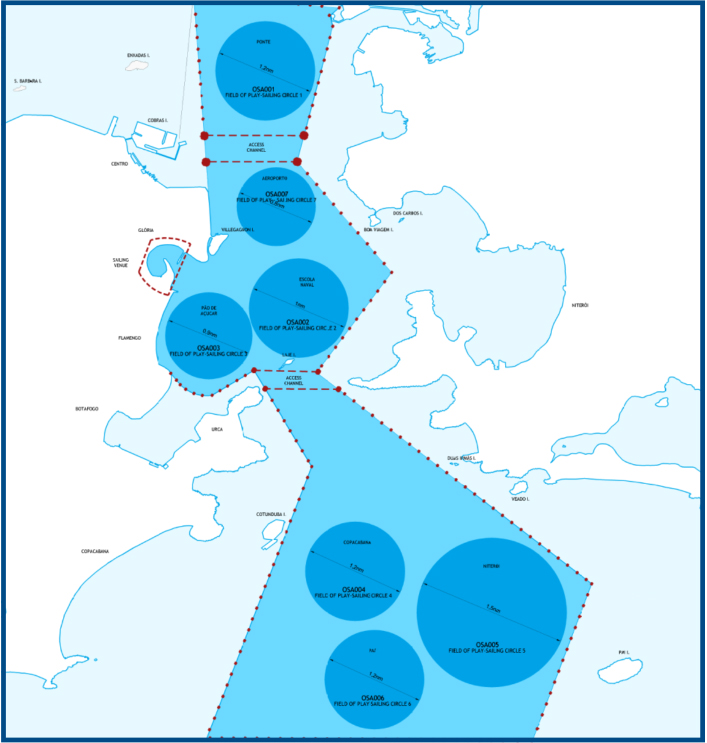
\includegraphics[width=0.6\textwidth]{16_OG_RaceAreasNOR.jpg}
  \caption{Sailing Races Areas. Olympic Games Rio 2016 \cite{instr_rio}.}
\label{fig:olymp_areas_rio} 
\end{figure}

\begin{figure}[ht]
  \centering
  \subfloat[Trapezoid Course ] {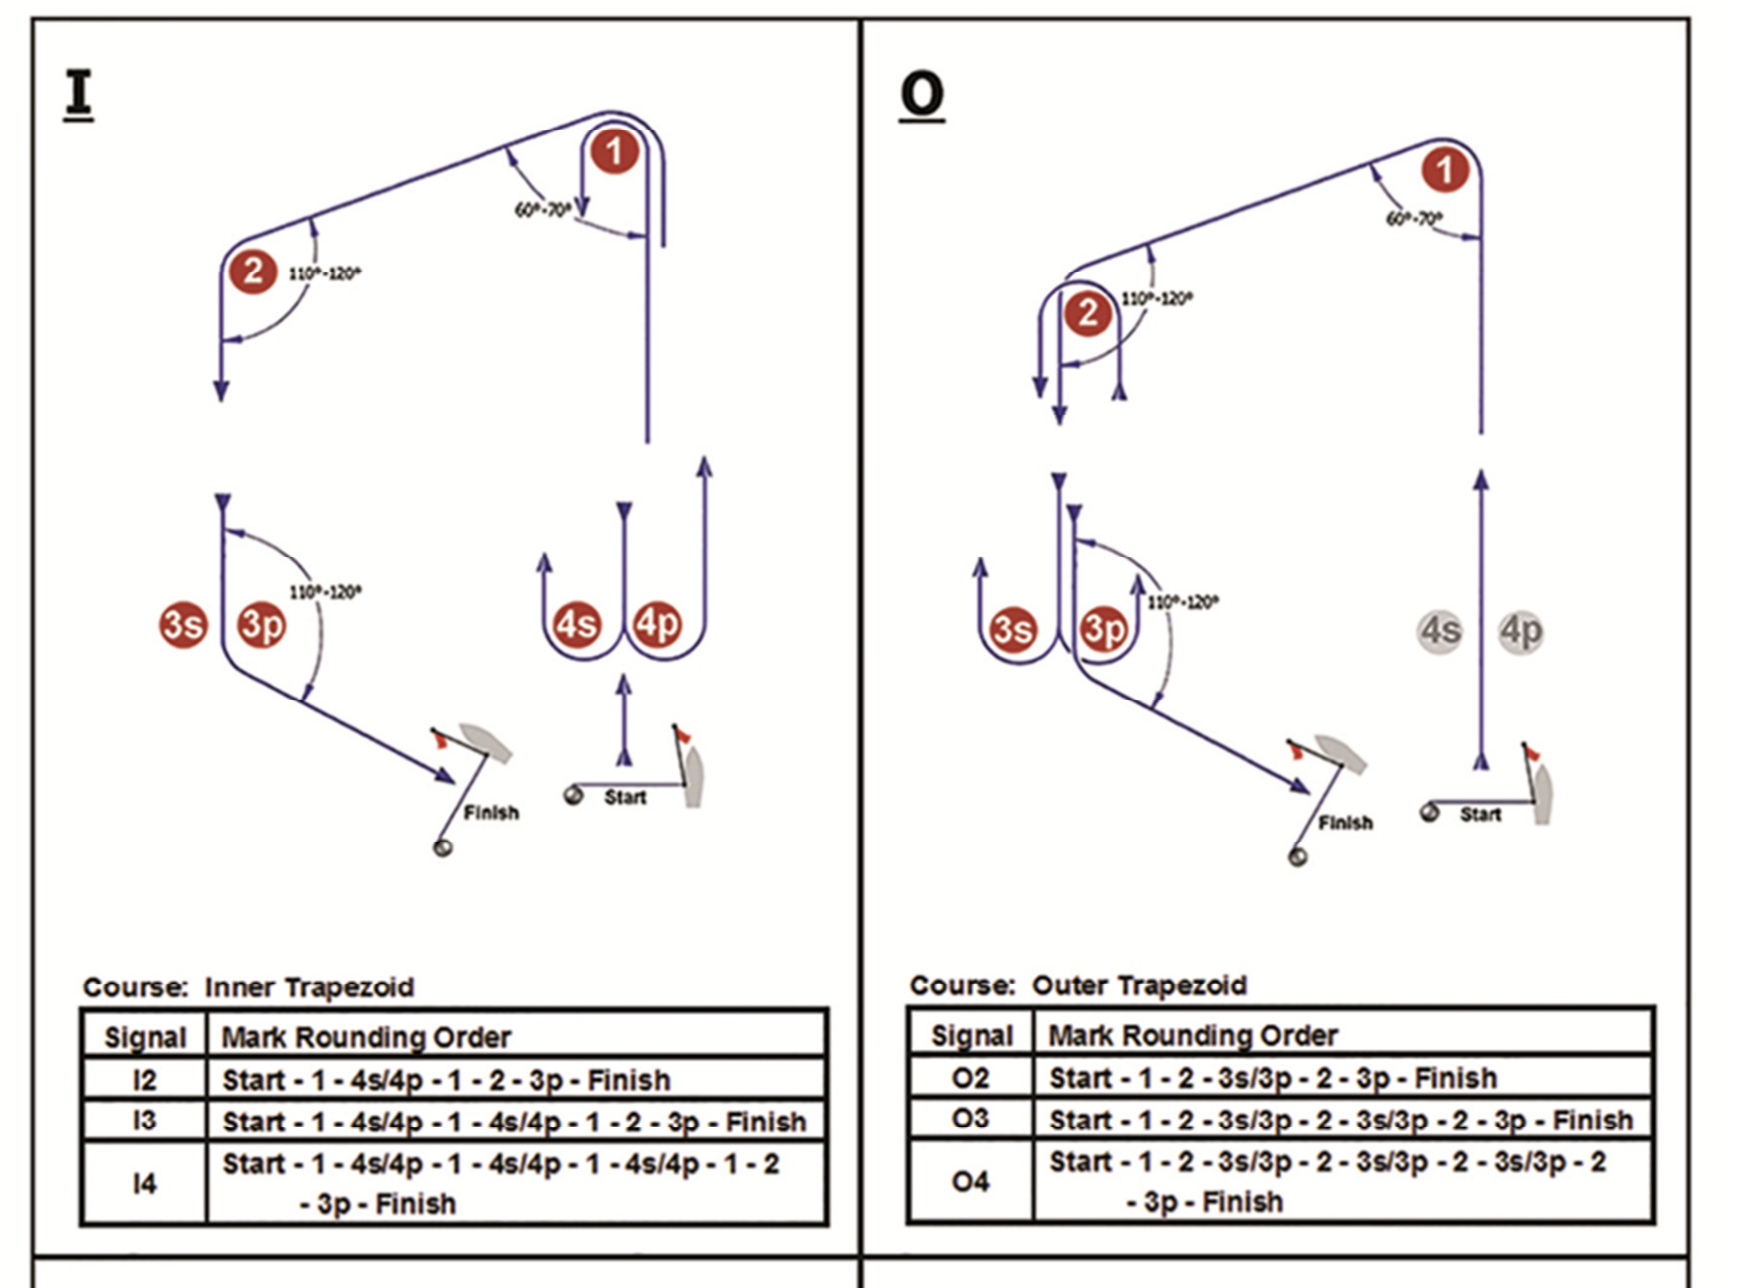
\includegraphics[width=0.53\textwidth]{trap_course.png}\label{fig:trap_c}}
  \hfill
  \subfloat[Windward / leeward course] {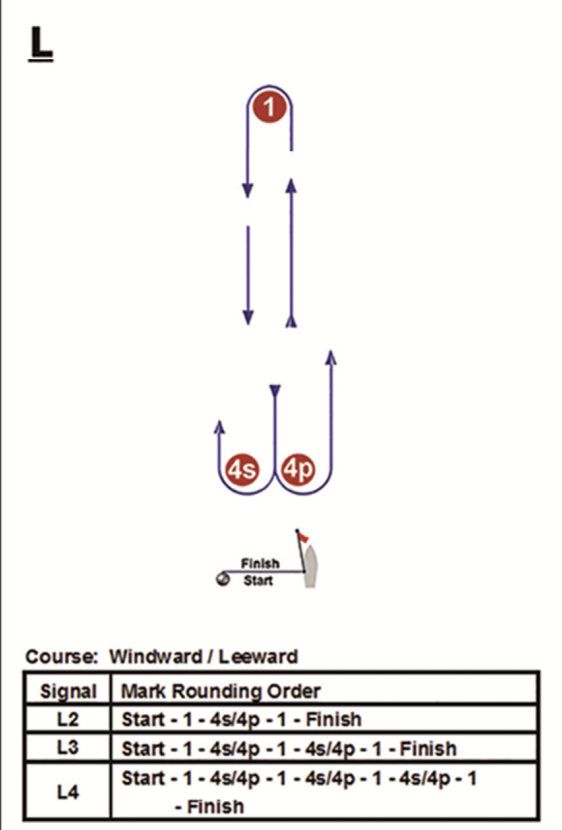
\includegraphics[width=0.25\textwidth]{l_w.png} \label{fig:wl_c}}
  \caption{Types of courses \cite{instr_rio}.}
\label{fig:typecourses} 
\end{figure}

The direction of the boat in respect to the wind determines the type of maneuvers and trajectory that must be followed. For example, the first leg of the trapezoid course runs against the wind and boats cannot displace towards it. The maneuvers used in this condition is shown in figure \ref{fig:tacking}, the trajectory forms a zig-zag pattern that can be started on the left- or on the right-hand side and each change on the heading direction is known as a tack. \par 

Even when the trajectory looks symmetrical, it is important to remember that the wind is not constant all the time and because during the competition, it is only allowed to have a maximum shift of 10 \degree \cite{race_pol}. It is important to understand how this shift affected the course, therefore the time of the course. So far there is no evidence to accept or reject this symmetric condition. This raises the question of \textit{which direction should be taken when the boat has to run against the wind}, in other words, \textit{which is the path with the minimal time to follow?}. \par \noindent
To answer this question athletes and coaches rely on their previous knowledge and experience to decide which is the starting direction. This previous knowledge is based on geographical characteristics around the area of the course and exposure to the site. Top athletes for the Olympic Games train in the site at least one year before the event.\par 
\begin{figure}[ht]
  \centering
  \subfloat[Tacking Maneuver \cite{denny2009float}.] {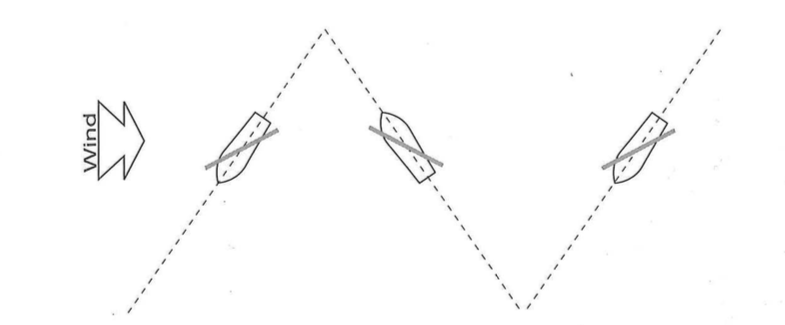
\includegraphics[width=0.65\linewidth]{tacking.png}\label{fig:tacking}}
  \hfill
   \centering
  \subfloat[Tacking maneuver]{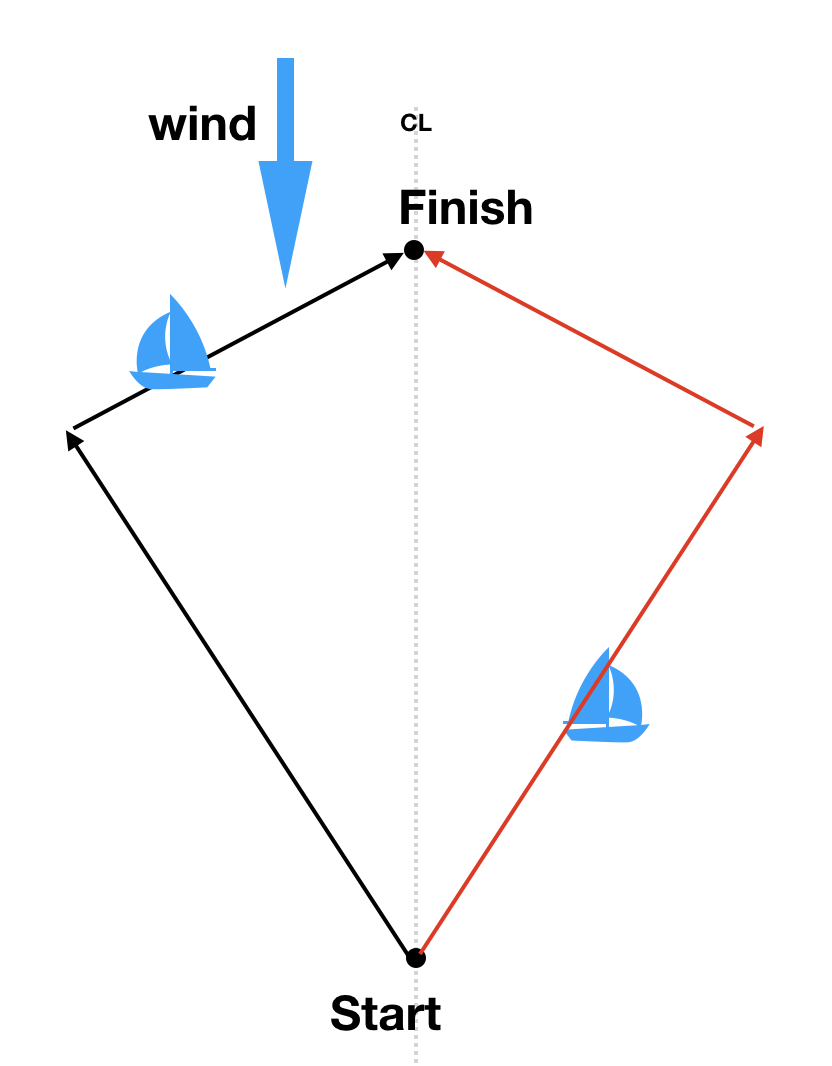
\includegraphics[width=0.3\linewidth]{images/upwind_sym.png}\label{tack_jib}}
  \caption{Tacking maneuver against the wind.}
\label{fig:tack_against_wind} 
\end{figure}

\section{Weather Forecast}
A weather forecast is calculated by supercomputers and updated every certain time according to the regions, usually every three hours. Due to its complexity different agencies and governments have developed models to predict the weather in global terms, so that local predictions could be made. This local predictions take into account the global model and adjusted according to local measurements allowing them to be updated every hour with a grid resolution of 3km by 3km \cite{warner2010numerical}. \par

Uncertain weather is a typical condition that yacht competitions and maritime transportation have to manage. In the case of yacht competitions, courses could take days, weeks or even months; like the \textit{Volvo Ocean Race}, which is an around the world. The path planning for this kind of boats has been researched especially by maritime and logistics sciences, a less number of publications can be found for yacht races and autonomous vehicles, and just a few numbers of researches refer to Olympic races. \par  

 Olympic races have a duration of maximum one hour inside a grid of size 2km by 2km and local forecast is updated every hour within a grid of 3km by 3km. Because of this, the information that coaches and athletes can access previously to the race does not match the characteristics and needs for them at first instance.\par
 Short course and long courses races are different. Short courses, for example, are more sensitive to random fluctuations \cite{philpott2001optimising}. Furthermore, the direction to take at the beginning of the competition could be the optimal just for a couple of minutes but not for the whole race. Time on Olympic sailing classes is critical to winning, but at the same time, a higher resolution on time and space for the weather is more costly in terms of computation effort for weather and the minimal time trajectory processing. The \textit{impact of a fine resolution vs a coarse on the time trajectories is unknown}. In the other hand, it is also unknown \textit{how small this resolution should be} in order to be significant for the  race.\par
 
 \section{The Aim of the Research}
This research proposes an algorithm to model sailing trajectories shaped by wind for Olympic Classes which %more specific for Laser (dinghies) competitions %and optimize it to obtain the minimal time for the Laser (Olympic class). 
can answer the question, \textit{Which is the optimal sailing route shaped by wind for the Laser (Olympic class) when the time and spatial resolution is set constant: every hour and every 10 min?, Which resolution is representative?}. The study suggests that the sensibility of the optimal route due to changes in the wind field and starting direction can define zones and shape the trajectory for minimal time paths. \par 

Moreover, it demonstrates the effects of 3 different time steps and spatial resolutions on the resulting trajectories with its times. This will be done by means of experiments using the optimization of the algorithm proposed. The results(simulations) obtained can be compared against the measurement data of the selected race. In this way, it is possible to identify the size of the differences and quantify the effect of the uncertain weather over the trajectory and times.\par 
%In other words,%the critical variables influenced by the wind that determine it.
%the study seek 
%To answer the question, What is the optimal sailing route for the Laser (Olympic class) shaped by wind. The objective is to analyze the sensibility of the optimal route due to changes on the wind field and start times. This will determine the zones and the shape trajectory of the optimal path. 
%and conditions that shape not only the optimal but the least route also. 
%To answer this question first, the physical model of yachts was reviewed. Despite the similarities between dinghies(Laser boats) and yachts, the physical model was adapted by adding two coefficients related with sails which indicate%the research focusing on dinghies is significantly lower as consequence adaptations have been made to represent
%how different is steering a dinghy from a yacht. Moreover, these adaptations are reflected on the %These adaptations are related with the
%Velocity Prediction Polar (VPP)diagram. By using the VPP and the wind intensity is possible to set the direction at which the dinghy reach is maximum velocity respect to the wind. This approach is known as Velocity Made Good (VMG).%  and to more specific and the use of sails
%Despite the similarities between dinghies and yachts, the research focusing on dinghies is significantly lower as consequence adaptations have been made to represent how it is steering, one of this is related with the VPP's and the use of sails. The same situation happens when the topic of research is related with optimal routes.  Since Olympic sailing is focused on the seamanship, the understanding of physical principals intends to provide or reveal hints that helps them to train and contest effectively regardless the location and routes. \newline

 \section{Terms, conditions, and limitations}
 %This report asses them 
%%these portable designs %the three concepts  
%with the multi-criteria analysis method to identify the most feasible design to enhance the force of the upper limb for people without impaired limbs. The design %with the higher score 
%obtained from the assessment was the powered exoskeleton with monitoring system.
The algorithm developed is limited to dinghies, the smallest and one of the most used boats on the Olympic classes. More specific, the Laser Class with motion over the XY plane. The 2D model proposed was validated by comparing the results of the simulations obtained against the results Laser races located at Hyères, France during 2018.\par \noindent The experiments to see the effects of the time step on the time and trajectory are the three wind conditions:% tested are: 
first, a constant wind intensity and direction along the area of the route; the second, considers a forecast wind field as time-space-dependent variable changing every 10 minutes over 1 km by 1km grid size without current and neglecting the wave disturbances and twisting effects on the sail; the last test %condition 
uses the wind measurements taken at 20 Hz during the competition. The algorithm developed is implemented on MATLAB\textsuperscript{\textregistered} and the optimization tool used is \cite{MatlabOTB}.\par 

Olympic Classes like the dinghy is not a widespread research topic. Besides most of the findings related to path optimization for boats are related to cargo ships and vessels, where the main objective is to minimize fuel costs because this ship can be set to navigate at a constant speed. A smaller amount of researches but more related to sports are the ones related to yachts; the influence of the wind is not the same as for the Olympic Classes. \par \noindent 
Another consideration is the movement of the sailor which was not considered as a variable since it was assumed that the athlete is skilled enough to keep the equilibrium of the boat and maximize speed without further complications. In the case of the crew weight, the simulations used the weight proposed by \cite{laser_opt}, which is between	55 and 70 kg.\par 

 \section{Report Structure}
The report is set as follows: chapter 2 refers to basic concepts and physics of sailboat; the forces and equation that governs its motion in general. The validation of the model, and how the wind model is integrated is reviewed in chapter 3. In chapter 4, the optimizer algorithm is explained as well as how the model is implemented with required modifications for the purposes of this research. The obtained results are analyzed in chapter 5; and finally, the conclusions and recommendations are described in chapter 6.\par 

%has been considering in the development of methods for the optimal path.
%The random fluctuation over the time is more sensitive on short courses rather long coursed.
%Taking good decisions on time depends on: the available data and processing time. The processing time refers to the time it takes to converted the available data into meaningful information. These two variables have been approaching by Different researchers to obtain 




%Because of this Philpott \cite{philpott2001optimising} describe a method for each condition to figure out the optimal path.  The weather variables in a short courses were considered to have a minimum spatial variation, although they enclose a random component due to its dependence over time.\\


%With this method the area and time have to being discretize, more over the it consider different states or possibles angles at which the wind will be directed. Which means that each location has to evaluate each of the states and find the optimal path among  \textit{n} stages.  The larger or the smaller the the discretization the more locations to solve according each stage, which seem that the computational effort will grow considerably since each leg has to be evaluated.  The paper does not mention the computational effort nor the difference of time that can be achieve by using it.Philpott \cite{philpott2001optimising}



\chapter{The physics behind sailboats} \label{ch:physics_sailboat}

Sailing boats are propelled mainly by wind. However, they displace through the water; in other words, sailboats move through 2 different fluids: water and wind. The mechanics of sailing have been known since the 1950s. Marchaj in 1979 review them and add information which is still being used for yacht design \cite{marchajaereo1979}.\par 

This chapter is focused on the motion of the sailboats, what are the physics concepts behind it, which forces interact in equilibrium and during motion. How the athlete takes part in this model and what other considerations are required to set-up the equations of motion. Since sailboats are governed by similar equations some adjustments are required to differentiate between yachts and lasers, these adjustments are explained on detail on later chapters. \par 
The equations of motion facilitate the identification of variables that can be used as a parameter to model the trajectory as well as to identify its limitations. These considerations are required to optimize the trajectory and obtain a minimal time path. \par
\section{The Interaction between the sailboat, water, and air} \label{sec:interaction_boat_environ}
The origin of the forces and momentum depend on the interaction of the elements of the sailboat with the 2 mediums; water and air. Some of these forces are clear, like the forces acting above the water surface which are produced by the wind and the interaction of it with the sails. These forces have to be balanced by the forces beneath the same surface; in this case, the water interacts with the hull, rudder, and keel. Therefore by adjusting the sail and the rudder, the only movable elements, the sailboat can hold a steady course.\par

Philpott explains how different elements, parts of the sailboat, interact with the surroundings and how they are used to control and attain the equilibrium during motion. Figure \ref{sailboat_terms} shows the most common elements and where are they located. Some of those elements can be manipulated by the seamanship, which means that the variables concerned can be controlled and therefore they are known as control variables \cite{philpott1993yacht}. \par

 \begin{figure}%[ht]
\centering
  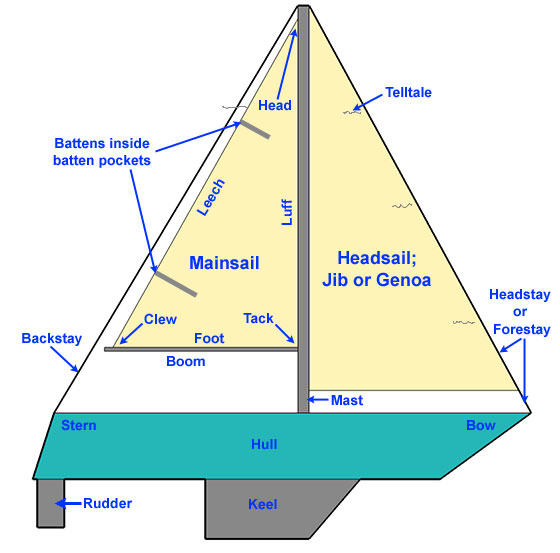
\includegraphics[width=0.4\linewidth]{sailboat_terms.jpg}
 \caption{Common sailboat terms \cite{sailboat_terms}. }
\label{sailboat_terms}
\end{figure}
\nomenclature[S]{$\lambda$}{Leeway Angle}
In order to steer a boat, the seamanship has to control the angle of the rudder, this interacts directly with the current, the direction obtained is called \textit{heading} and these two, rudder and current, generate forces that influence the boat to \textit{yaw}. \par
Due to the wind direction, mainly, the boat slips sideways and this effect is known as \textit{leeway}. The difference in course comparing with the heading is expressed as \textit{leeway angle ($\lambda$)}. %, which can be see in the figure \ref{forces_m} \textit{C}.
The sails adjustment is known as trim; when the trim reduce the area of the sail then the seaman is \textit{reefing}, most of the time this term refers to when the size of the sails is changing.  Reefing under sail allows the seamanship to control the wind intensity. \par
\nomenclature[S]{$M_{R}$}{Righting Moment}
The wind over the sails generates a force and an angle called \textit{heel angle}; which can be seen in figure \ref{forces_m} \textit{B}, this decreases the driving force. Under those circumstances, a moment is generated and to neutralize it, the seamanship generates a \textit{righting moment} (\textit{ $M_{R}$}) by standing on the windward side of the boat to produce it\cite{philpott1993yacht}. 
As a result of these forces, the velocity could be optimal or not. \cite{larsonprinciples} relates the factors and forces proposed in\cite{philpott1993yacht} in terms of forces and resistances, indicating how the dynamics of each of the mediums, water, and air, interact to keep the balance (and be capable to maximize the boat's speed). Therefore, the forces and resistances are related as showed below: \par 
\begin{itemize}  \label{milgramforces}
 \setlength \itemsep{0em}
\item Aerodynamic driving forces = Hydrodynamic resistance;
\item Aerodynamic side force = Hydrodynamic side force;
\item Aerodynamic heeling moment=Hydrodynamic (static) righting moment.
\end{itemize}
An important assumption made by  \cite{philpott1993yacht} and \cite{larsonprinciples} to keep the analysis of the boat in 2 dimensions is that vertical forces are in balance always, same as the pitching moment; Figure \ref{forces_m} \textbf{c} shows the only forces that act when this assumption is made; additionally 2 angles are shown, one of then refers to the wind.\par
\nomenclature[A]{DOF}{Degrees of freedom}
\section{Planes of motion} \label{sec:planes_motio}
Sailing boats are considered rigid bodies that can move in a three-dimensional space; figure \ref{DOF} shows the 6 fundamental types of motion or degrees of freedom (DOF)  with the names and axis where they are referred: three translations and three rotations. \par 
It also shows the water surface which is represented by the plane \textit{XY} and the orientation of the sailboat shows the positive direction of the three axes which follow the right-hand orthogonal system. Thus, \textit{X-axis} is positive in the direction of the motion, \textit{Y} is positive to port or left side of the sailboat and \textit{Z} is positive upwards. In the case of the \textit{Y-axis}, the negative direction or right side of the sailboat is known as starboard.  Besides, for future references, the speed of the boat is along the \textit{X-axis}. These six DOF correspond to three forces and three moments which are going to explain in the next section. \par 
\begin{figure} %[ht]
\centering
  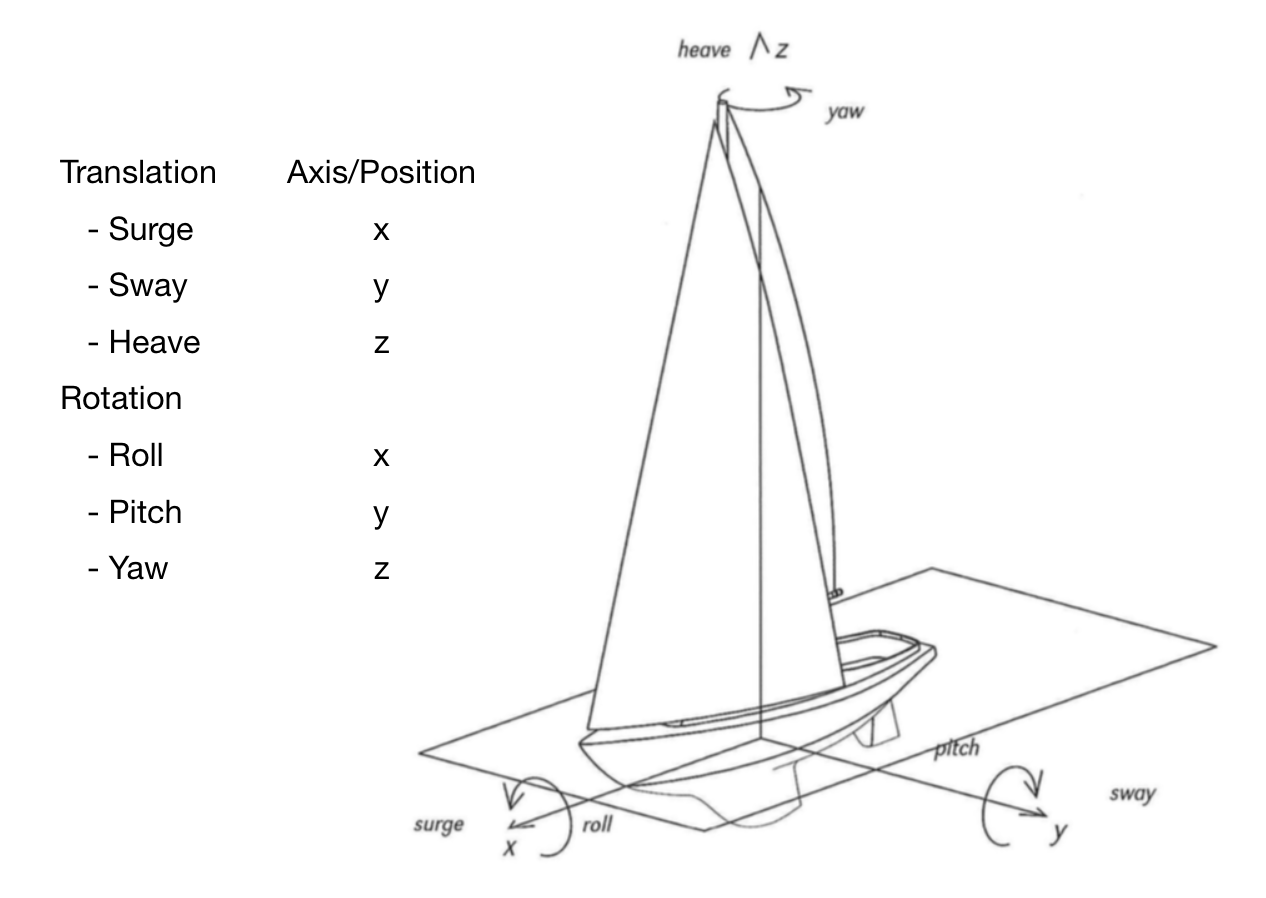
\includegraphics[width=0.7\linewidth]{dof_foss_modif.png}
 \caption{Degrees of freedom of a boat, clockwise reference system \textit{XYZ} \cite{fossati2009aero}. }
\label{DOF}
\end{figure}

%The information provided in the figure %To represent the position, velocities and forces, a set of vectors are defined in 

Because the sailboat interacts between two fluids not only do they generate forces but also resistances in both mediums. It is important to know how the elements are named and which words are related with a specific axis and  %These simple concepts are useful to understand how the equilibrium is generated in the static condition, 
which elements interact on it and how it is conserved when the sailboat moves from one point to another. \par 

\section{Hydrodynamic and Aerodynamic Forces and Momentum} \label{section:forces_moment}
The static and dynamic balance of any type of boat is based on Newton's second law. However, when the boat moves, a dynamic situation, it is the winds' velocity that leads to this equilibrium. Because the sailboat interacts between two fluids they not only generate forces but also resistances.
\nomenclature[S]{$F_{A}$}{Total Aerodynamic Force}
\nomenclature[S]{$F_{H_{TOT}}$}{Total Hydrodynamic Force}
The next equations basically show that the total aerodynamic force ($F_{A}$) is equal and opposite to the total hydrodynamic force ($F_{H_{TOT}}$). \par
From section \ref{sec:planes_motio}, a set of vectors can be defined to represent the position, velocities, and forces. The notation used here is similar to the one used by the \acrfull{sname} %\acrlong{sname} (\textit{\acrshort{sname}})%the Society of Naval Architects and Marine Engineers (\textit{SNAME}) 
because different authors use different notation, this work is intended to stay close to the norm which is shown in table \ref{table:SNAME_notation}, this notation refers to the body-fixed reference frame.
\nomenclature[A]{\textbf{SNAME}}{Society of Naval Architects and Marine Engineers}
\begin{table}%[]
    \centering
    \begin{tabular}{c|c|c|c}
    \hline
          Motion/Rotation & Force/Moment & Linear/Angular vel & Position/Angles   \\
    \hline 
         Surge(X-axis) & X & u & x \\  
         Sway (Y-axis) & Y & v & y \\
         Heave(Z-axis) & Z & w & z \\
         Roll (X-axis) & K & p & $\phi$ \\
         Pitch (Y-axis) & M & q & $\theta$\\
         Yaw (Z-axis) & N & r & $\psi$\\
    \end{tabular}
    \caption{\acrshort{sname}'s notation for motion components \cite{Alves2014ASailboat}}
    \label{table:SNAME_notation}
\end{table}

\nomenclature[S]{$\theta$}{Pitch Angle}
\nomenclature[S]{$\phi$}{Roll Angle}
\nomenclature[S]{$\psi$}{Yaw Angle}

\subsection{Wind and the Velocity Triangle} \label{sec:wind_vel_trian}
\nomenclature[S]{$V_{tw}$}{True Wind Velocity}
\nomenclature[S]{$\beta_{tw}$}{True Wind Angle}
\nomenclature[S]{$\kappa$}{Exponent for wind velocity at different height [1/7,1/4]}
In sailing, the wind is characterized by its speed and direction and it is defined as \textit{true wind velocity ($V_{tw}$)} and \textit{true wind angle ($\beta_{tw}$)}. Because it also interacts with the water surface, in some cases its intensity depends on the height where it was measured, to know its value at a different height it is estimated by equation \ref{eq:wind_h}. According to \cite{claughton1998sailing} the exponent $\kappa$ has a value between 1/7 and 1/14, and; the reference height for measurements is 10m above the water surface. \par 
\begin{equation}\label{eq:wind_h}
    V_{tw}(Z)=V_{tw}(Z_{ref}) \cdot \bigg( \frac{Z}{Z_{ref}} \bigg)^\kappa
\end{equation}

The steady motion of the sailboat not only depends on the balance of forces but also on the relation between velocities, boat, and wind, mainly. This interaction is represented by the velocity triangle shown in figure \ref{vel_triangle}. The triangle introduces the apparent wind velocity ($V_{aw}$) and angle ($\beta_{aw}$).\par 
\nomenclature[S]{$V_{aw}$}{Apparent Wind Velocity}
\nomenclature[S]{$\beta_{aw}$}{Apparent Wind Angle}
%\begin{figure}[ht]
%\centering
%  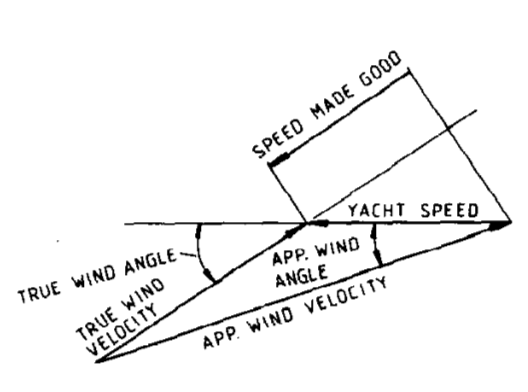
\includegraphics[width=0.65\linewidth]{Larsson_triang_vel.png}
% \caption{Velocity triangle  \cite{larsonprinciples}. }
%\label{vel_triangle_old}
%\end{figure}

%option figure to REVIEW
\begin{figure} %[ht]
  \centering
  \subfloat[Velocity triangle  \cite{larsonprinciples}. ]{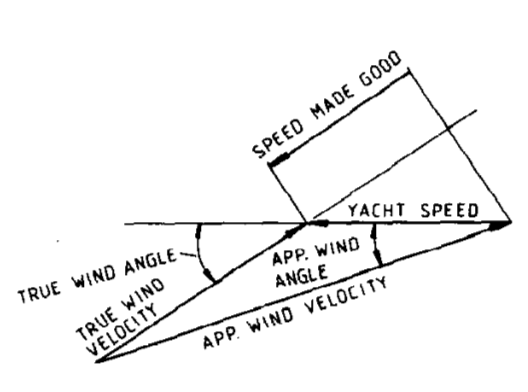
\includegraphics[width=0.45\linewidth]{Larsson_triang_vel.png}\label{vel_triangle}}
  \hfill
  \subfloat[Angles and course direction \cite{marchajaereo1979}.]{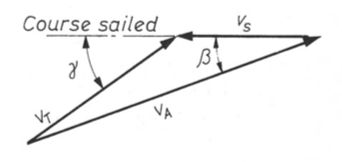
\includegraphics[width=0.45\hsize]{geo_vel_triangle}\label{fig:velTriang_sailCourse}}
  \caption{Velocity Triangle and angle directions of wind and $\lambda$  \cite{marchajaereo1979}, \cite{larsonprinciples}.}
\label{fig:Vel_Trian_Ang} 
\end{figure}

\nomenclature[S]{$V_{aw}$}{Apparent wind velocity}
%\nomenclature[A]{SGP}{Some Random Acronym}
%\newacronym{gcd}{GCD}{Greatest Common Divisor}
%EXAMPLE \acrlong{gcd} \acrfull{gcd} \acrshort{gcd} \acronymtype 

\nomenclature[S]{$\Theta$}{Heel Angle}
\nomenclature[S]{$\gamma$}{Course Angle}
\nomenclature[A]{$CE$}{Center of Effort}
\nomenclature[S]{$V_{boat}$}{Boat's velocity}

The $V_{aw}$ and $\beta_{aw}$ result from the vector summation of the true wind ($V_{tw}$) and sailboat's ($V_{boat}$) velocity, \ref{eq:vel_appVector}; a more complete estimation of them uses the heel angle ($\Theta$), equations \ref{eq:app_angle} and \ref{eq:app_angle} show how to calculate them. These equations include the heel angle because $V_{aw}$ is used to calculate some sail force coefficients which are specified at the center of effort (\textit{CE}), its location is about 40\% at the mast height. The $\beta_{aw}$ incorporated the leeway angle ($\lambda$), which value is usually less than 6\degree \cite{philpott1993yacht},\cite{claughton1998sailing}. Subsequently, the course angle $\gamma$ is complementary to the $\beta_{aw}$ when $\lambda$ is not bigger than 6\degree \ref{fig:velTriang_sailCourse}. \par
\begin{equation}\label{eq:vel_appVector}
    \vv{V_{aw}}=\vv{V_{tw}}-\vv{V_{boat}}
\end{equation}

\begin{equation} \label{eq:app_angle}
    \beta_{aw}=tan^{-1} \bigg( \frac{ V_{tw} sin \beta_{tw} cos \Theta }{ V_{tw} cos \beta_{tw} + V_{boat}} \bigg)
\end{equation}
\newline
\begin{equation} \label{eq:ap_vel}
    V_{aw}=  \sqrt{ (V_{tw} sin \beta_{tw} cos \Theta)^2 + (V_{tw} cos \beta_{tw} + V_{boat})^2}
\end{equation}

\subsection {Equilibrium Equations} \label{sec:equil_equat}
In the static condition, equilibrium is reached when the summation of all the forces and momentum equals zero. In figure \ref{forces_m} these forces are located according to the planes where they act, the names of them and the fluid that drives them. In addition to the forces and momentum, there are 4 angles to consider. Another observation is how the position and weight of the athlete are incorporated in the equilibrium equations. \par 

\nomenclature[A]{$\textit{F}$}{Force}
\nomenclature[S]{$F_{R}$}{Driving Force}
\nomenclature[S]{$R$}{Water Resistance}
\nomenclature[S]{$F_{H}$}{Heeling Force}

The equations of forces(\textit{F}) by plane in equilibrium are:
\begin{equation}\label{eq:force_x}
    \text{(Surge, x  \space axis)  \space} F_{R}=R \\
\end{equation}
\begin{equation}\label{eq:force_y}
    \text{(Sway, y\space axis) \space } \space F_{H,lat}=F_{S,lat}\\
\end{equation}
\begin{equation}\label{eq:force_z}
    \text{(Heave, z\space axis)  } \space F_{V}=F_{VW}
\end{equation}
And those for the momentum (\textit{M}) in equilibrium are:
\begin{equation}\label{eq:m_x}
    \text{(Roll, x  \space axis) \space } M_{R}=M_{H} \\
\end{equation}
\begin{equation}\label{eq:m_y}
    \text{(Pitch, y \space axis)  } \space M_{PA}=F_{PW}\\
\end{equation}
\begin{equation}\label{eq:m_z}
    \text{(Yaw, z \space axis)  } \space M_{YW}=M_{YL}
\end{equation}

 \begin{figure}[ht]
\centering
  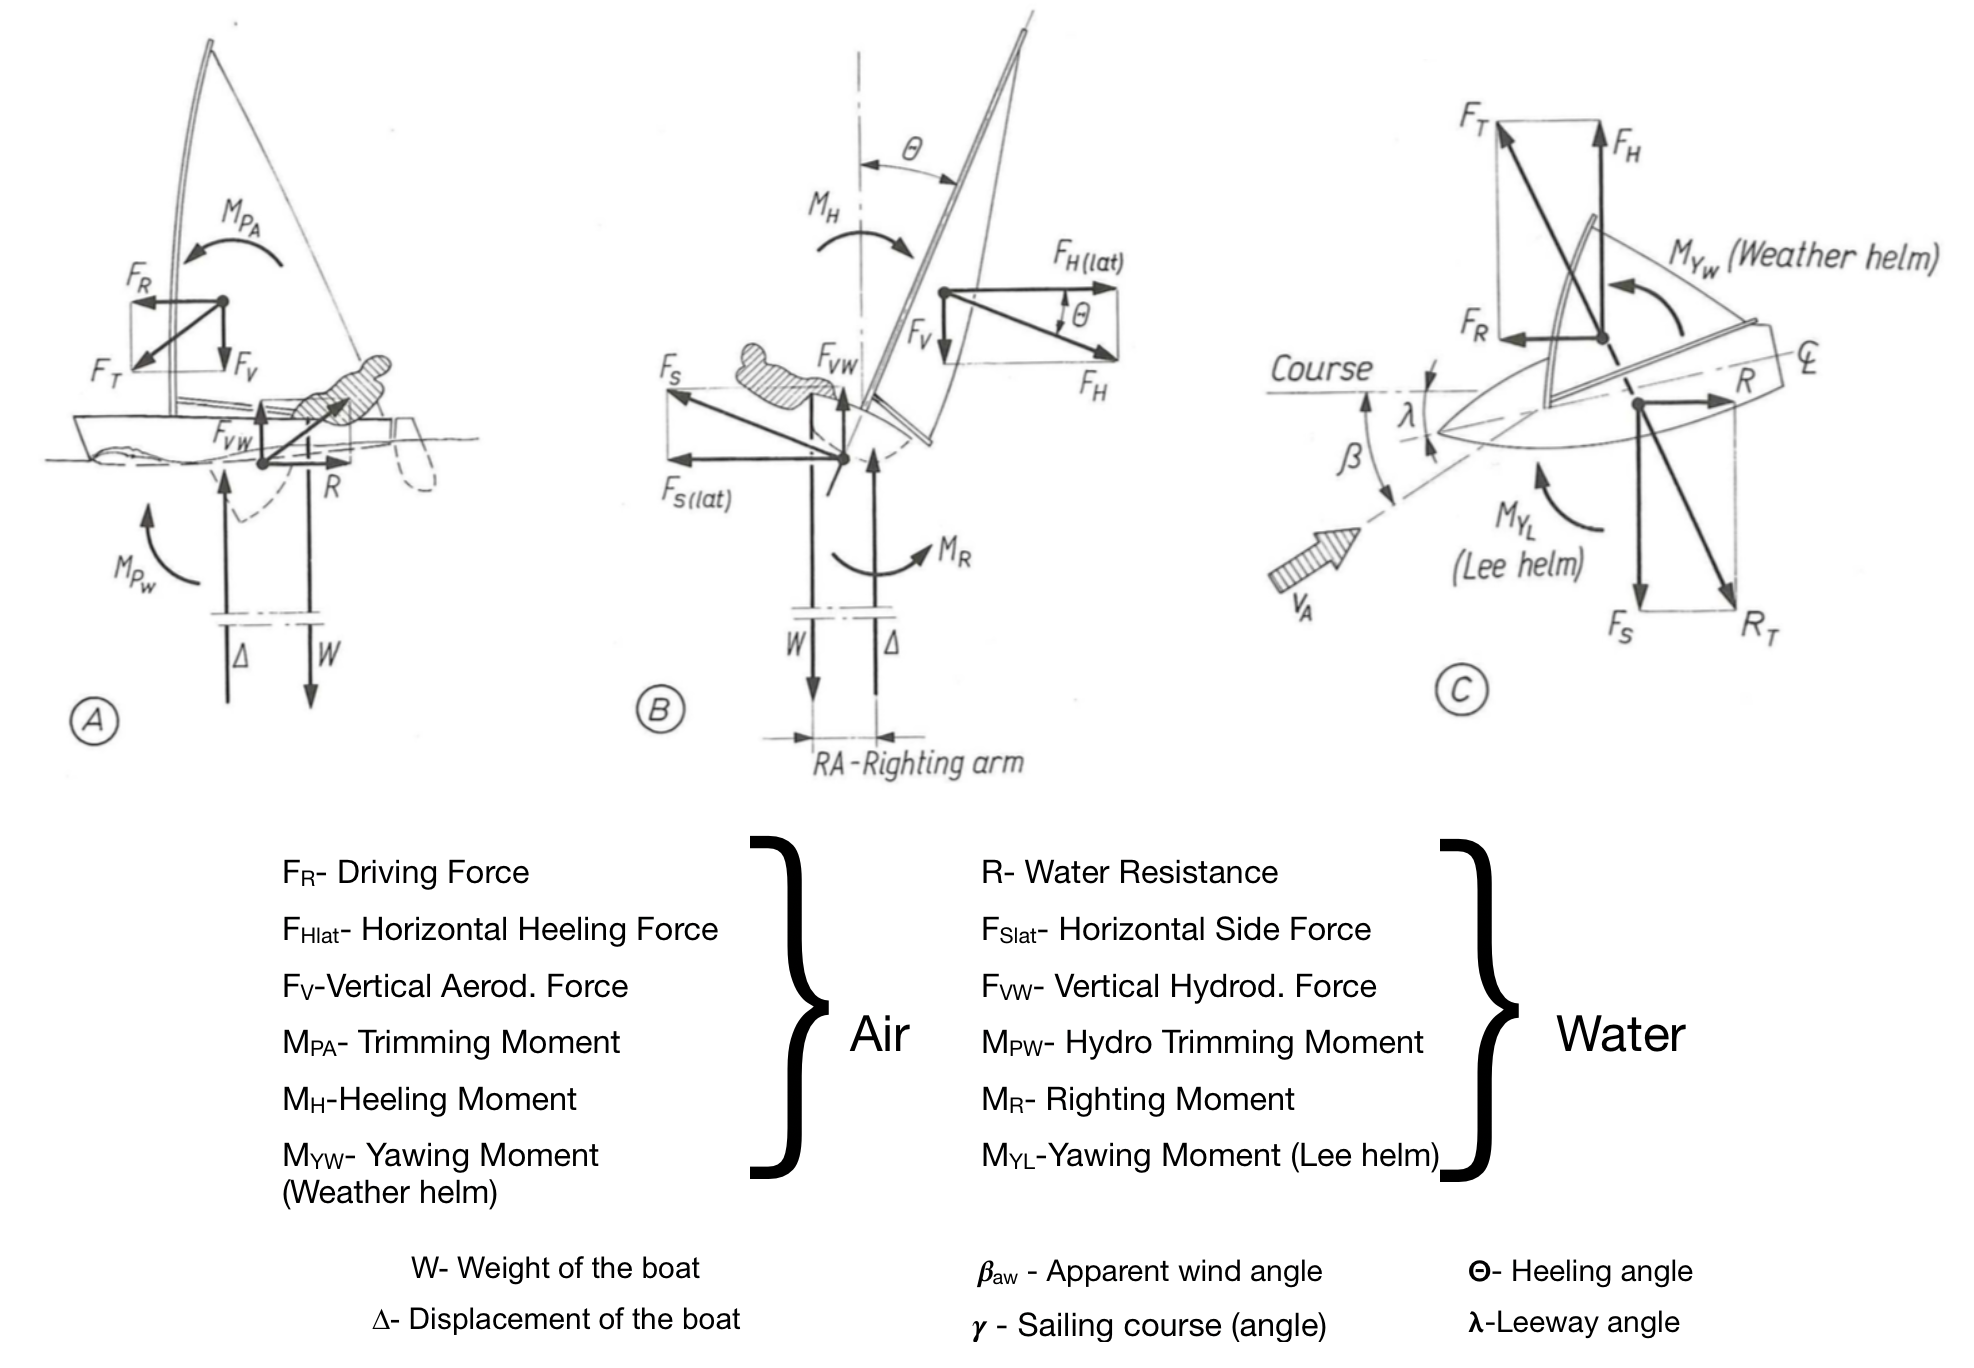
\includegraphics[width=.97\linewidth]{marchaj_forcesM.png}
 \caption{Equilibrium of forces and moments in steady-state sailing condition \cite{marchajaereo1979} }
\label{forces_m}
\end{figure}

\subsection{Aerodynamic Forces and Resistances} \label{sec:aero_forces}
\nomenclature[S]{$F_{S}$}{Hydrodynamic Side Force}
\nomenclature[S]{D}{Drag Force}
\nomenclature[S]{L}{Lift Force}

The force that drives motion of the sailboat is the driving force($F_{R}$); figure \ref{forces_m} \textit{B} shows the force that causes the drift (heel) of the sailboat is the heeling force ($F_{H}$). The motion of the sailboat happens when $F_{R}$ beat the hull resistance (\textit{R}); while in the \textit{ZY} plane the balance of the forces happens when $F_{H}$ equals the hydrodynamic side force ($F_{S}$), which is produced by the effect of the water over the hull. Then:\par 
\begin{figure} [htb!]
    \centering
    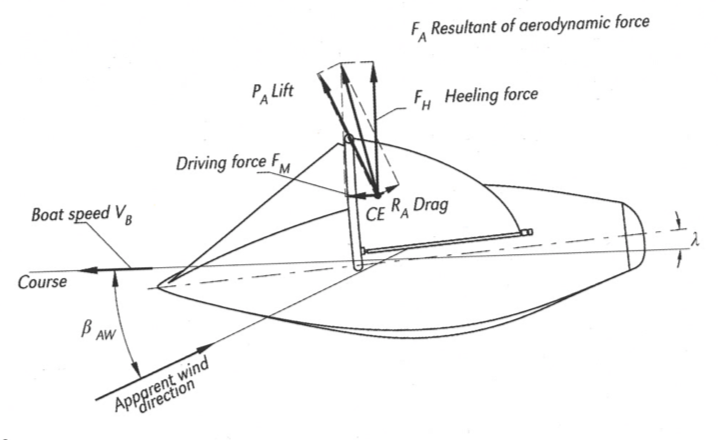
\includegraphics[width=.5\linewidth]{Ftot_aereo.png}
    \caption{Total Aerodynamic Forces \cite{fossati2009aero}}
    \label{fig:Ftot_aereo}
\end{figure}
%( Because $F_{A}$ result from $F_{R}$, parallel to the \textit{apparent wind} direction and $F_{H}$ perpendicular to $F_{R}$. Under balance the variables related to them are:)
\begin{multline}
\\
F_{A}=F_{R}(\parallel V_{aw}) + F_{H}(\bot F_{R} )\\
F_{R}=F_{R}(V_{aw},\beta_{aw}, \Theta) \\
F_{H}=F_{R}(V_{aw},\beta_{aw}, \Theta) \\
F_{S_{lat}}=F_{S}(V_{boat},\lambda, \Theta) \\
R=R(V_{boat},\lambda, \Theta)\\  
\end{multline}
%th they depend on the $V_{aw}$ and $\beta_{a}$; while $F_{S}$ and \textit{R} depend on $V_{boat}$ and $\lambda$. 
Due to the dependency on velocities, $F_{R}$ and $F_{H}$ generate drag (\textit{D}) and lift (\textit{L}) forces acting normal to the center plane of the hull and mast and they are integrated into the forces, figure \ref{fig:Ftot_aereo}, according to \cite{philpott1993yacht} and \cite{claughton1998sailing} as: \par 
\begin{equation} \label{eq:Fr_LD}
    F_{R}=L sin \beta_{a} - D cos \beta_{a}
\end{equation}
\begin{equation} \label{eq:Fh_LD}
    F_{H}=(L cos \beta_{aw} + D sin \beta_{aw}) cos\Theta
\end{equation}
\\ \textit{D} and \textit{L} depends not only on  the sail area (\textit{$A_{s}$)}, $V_{aw}$, and fluid density ($\rho_{a}$), in this case, air, but also on coefficients which depends on the trim and flatness of the sail \cite{philpott1993yacht}, \cite{carrico17symp}, \cite{day2017performance}; these last, are under the control of the seamanship. \textit{D} and \textit{L}  are expressed in those terms as follow: \par
\nomenclature[S]{$\rho_{a}$}{Air Density}
\begin{equation} \label{eq:Lift}
  L=qA_{s}C_{t}  
\end{equation}
\begin{equation} \label{eq:Draf}
    D=qA_{s}C_{d}  
\end{equation}
\begin{equation} \label{eq:dynamic_press}
    q=\frac{1}{2}\rho_{a} V_{aw}^2
\end{equation}
\begin{equation} \label{eq:Cd}
    C_{d}=C_{d}(\beta_{a},trim, flatness)
\end{equation}
\begin{equation} \label{eq:Ct}
    C_{t}=C_{t}(\beta_{a},trim, flatness)
\end{equation}
where:
\begin{itemize} \label{ae_symbols}
    \item $\rho_{a}$ air density approx. 1.225 $kg/m^3$.
    \item $A_{s}$ is the area of the sail.
\end{itemize}

\nomenclature[S]{$A_{s}$}{Sail Area}
\nomenclature[S]{$F_{ms}$}{Driven Sail Force}
\nomenclature[S]{$F_{ss}$}{Side Sail Force}
\nomenclature[S]{$q$}{Dynamic Pressure}

$C_{d}$ and $C_{t}$ values are obtained from tables or graphics and their range is over (0,1), later on, this is going to be explained in detail. \par 
$F_{R}$ is the total force applied on the sail which can be decomposed in 2 more forces; a driven force $F_{ms}$ and a side force $F_{ss}$ expressed in the terms mentioned before as:\par
\begin{equation}\label{eq:drive_sail_force}
    F_{ms}= (L cos \beta_{aw}+ D sin \beta_{aw})cos \Theta sin \lambda + (L sin \beta_{aw}-D cos\beta_{aw})cos \lambda
\end{equation}
\begin{equation}\label{eq:side_sail_force}
    F_{ss}=(L cos \beta_{aw}+ D sin \beta_{aw})cos \Theta cos \lambda - (L sin \beta_{aw}-D cos\beta_{aw})sin \lambda
\end{equation}
%%%NEW SUBSECTION %%%
\subsection {Hydrodynamic Forces and Resistances} \label{sec:hydroforces}
$F_{H_{TOT}}$ is equivalent to $F_{A}$ with the difference that they result from the interaction with the water. In this case, \textit{R}, a drag force (resistance) oppose the motion of the sailboat as shown in figure \ref{fig:Ftot_hydro}; and the horizontal side force $F_{S_{lat}}$, is a lift force acting over the hull and keel. Most of the information related with the modeling of the hull and keel is based on experimental data. % which is used to calibrate the theoretical model.
Then the drag generated by the hull is the result of the  upright, heeled and induced resistances \cite{philpott1993yacht}.\par

\nomenclature[S]{$F_{S_{lat}}$}{Horizontal Side Force}
\nomenclature[S]{$C_{d}$}{Drag Coefficient}
\nomenclature[S]{$C_{t}$}{Lift Coefficient}

\begin{equation}
    F_{H_{TOT}}=R(\parallel( -V_{aw})) + F_{S_{lat}}(\bot R )\\
\end{equation}

\begin{figure}
    \centering
    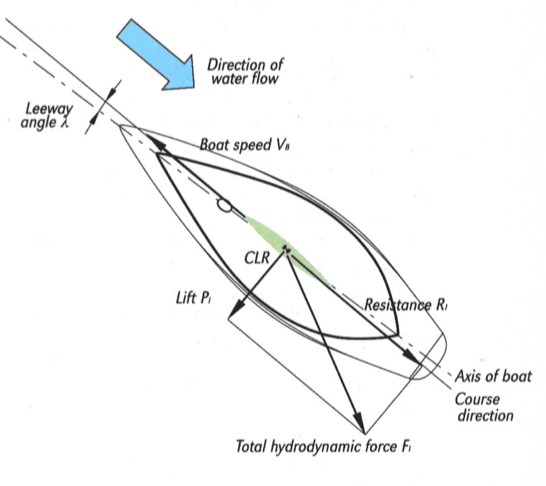
\includegraphics[width=.5\linewidth]{Ftot_hydro.png}
    \caption{Total Hydrodynamic forces. \cite{fossati2009aero}}
    \label{fig:Ftot_hydro}
\end{figure}

The upright resistance is produced by the hull drag and when $\lambda$ is zero. It is constituted by the friction generated by the water viscosity and wave drag, dissipation of energy in form of waves due to the shape of the hull. The formula to calculate these two frictional forces, equation \ref{eq:water_fric} and \ref{eq:wave_fric} is similar to the one from classical hydrodynamics, the difference is the coefficients. $C_{f}$ depends on $V_{boat}$ and its waterline length while $C_{w}$ depends on the hull shape and Froude number (\textit{Fr}), which considers the $V_{boat}$ and length of the sailboat; however, it is often determined by tests evaluations.
\nomenclature[S]{$C_{f}$}{Hydrodynamic Coefficient for the waterline length}
\nomenclature[S]{$C_{w}$}{Hydrodynamic Coefficient for the hull shape}
\nomenclature[S]{$F_{i}$}{Induced and heeled resistance forces}

\begin{equation}\label{eq:water_fric}
 F_{f}=\frac{1}{2}\rho_{w} C_{f} A_{w} V_{boat}^2
\end{equation}
\begin{equation}\label{eq:wave_fric}
 F_{w}=\frac{1}{2}\rho_{w} C_{w} A_{w} V_{boat}^2
\end{equation}
where:
\begin{itemize} \label{R_symbols}
    \item $\rho_{w}$ water density approx. 1000 $kg/m^3$.
    \item $A_{w}$ is the wetted surface area of the sailboat
\end{itemize}
\nomenclature[S]{$A_{w}$}{Wetted Surface Area of the sailboat}
\nomenclature[S]{$\rho_{w}$}{Water Density}

The induced and heeled resistances are combined and related with the heel and $\lambda$, its formula also depends on $V_{boat}$. Due to its complex derivation and different versions the expression is going to be set as; $F_{i}(\lambda,\Theta,V_{boat})$, for the purpose of this work. Then \textit{R} due to hydraulic resistances is calculated as: \par 
\begin{equation} \label{eq:R_total}
    R=F_{f}+F_{w}+F_{i}
\end{equation}

\nomenclature[S]{$S$}{Total Side Force}

In the case of $F_{S_{lat}}$, it depends also on 3 resistances generated by the hull, the lifting surface of the rudder and keel; these 2 last are the more significant and they are also perpendicular to the velocity. This total side force (\textit{S}), on the water plane, depends on the plan area of the keel and rudder and in 2 coefficients, respectively.  Thus, it is estimated as: \par 

\begin{equation}
    S=\frac{1}{2} \rho_{w} V_{boat}^2(C_{rudder}A_{rudder}+C_{keel}A_{keel})cos \Theta
\end{equation}.

\nomenclature[S]{$C_{rudder}$}{Rudder Coefficient}
\nomenclature[S]{$C_{keel}$}{Keel Coefficient}
\nomenclature[S]{$A_{rudder}$}{Rudder Surface Area}
\nomenclature[S]{$A_{keel}$}{Keel Surface Area}

The shape, of the rudder and keel, in conjunction with the angle of attack, has implication on each coefficients respectively. %$C_{rudder}$ and $C_{keel}$, each depends on the the shape and angle of attack of each. 
The angle of the rudder ($\beta_{r}$) is the angle it makes with the center line of the sailboat. Each angle of attack (\textit{$\beta_{i_{a}}$})is determined as: \par 
\nomenclature[S]{$\beta_{r}$}{Rudder Angle}
\nomenclature[S]{$\beta_{r_{a}}$}{Rudder Angle of Attack}
\nomenclature[S]{$\beta_{k_{a}}$}{Keel Angle of Attack}
\begin{equation}
    \beta_{r_{a}}=tan ^{-1} (cos \Theta cos \lambda + \beta_{r})
\end{equation}
\begin{equation}
    \beta_{k_{a}}=tan ^{-1} (cos \Theta cos \lambda )
\end{equation}

$F_{S_{lat}}$ in equilibrium can be estimated based by using $F_{H}$ which generates a reaction force below the water surface, then: %
which us know as horizontal side force $F_{S_{lat}}$ and it is determined as follow: \par
\begin{equation}
    F_{Slat}= F_{H}cos \Theta
\end{equation}

%% new section
\nomenclature[A]{$CLR$}{Center of Lateral Resistance}
\nomenclature[S]{$M_{R}$}{Righting Moment}
\nomenclature[S]{$W$}{Weight}

\subsection{Momentum at the sailboat model} \label{sec:momentum_types}
Because $F_{A}$ is applied at \textit{CE}, above the waterline and located over the sails area; and $F_{H_Tot}$ at the center of lateral resistance (\textit{CLR}), defined below the waterline. The moments generated over the sailboat depends on these 4 variables. For example, the \textit{righting moment ($M_{R}$)}, figure \ref{forces_m} \textit{B} is counterbalanced as next: 
\begin{equation}\label{eq:right_mom}
    M_{R}=F_{H}(CE-CLR)_{z}=W \cdot RA
\end{equation}
where:\par
\begin{itemize}
    \item $(CE-CLR)_{z}$ is the heeling arm or the vertical distance between \textit{CE} and \textit{CLR} when $F_{H}$ is perpendicular to it.
    \item W = weight of the boat.
    \item RA = Righting arm or the horizontal distance between the \textit{W} and the \textit{Z} axis.
\end{itemize}
\nomenclature[S]{RA}{Righting Arm}
\nomenclature[S]{$W_{c}$}{Weight of the crew}
This expression does not take into account the weight of the crew. The moment generated by the crew weight is given by the weight of the crew (\textit{$W_{c}$})) and its relative position to the centerline of the boat, which is expressed by a variable known as \textit{$y_{c}$}. This variable has a range value of [-1,1], and if the crew is in the centerline then its value is zero. Another factor to considers is $\Theta$. So the moment generated by the crew according to Philpott \cite{philpott1993yacht} is: \par 
 \nomenclature[S]{$y_{c}$}{Crew position on Y-axis from the centerline}
 \nomenclature[S]{$M_{c}$}{Crew Moment}
 
\begin{equation}\label{eq:Moment_crew}
    M_{c} = y_{c} W_{c} Y_{max} cos \Theta
\end{equation} 
\begin{equation} \label{eq:Mcrew_dist}
    Y_{max} = \frac{1}{2} beam(width)_{sailboat}
\end{equation}

\nomenclature[S]{$M_{R_{TOT}}$}{Total Righting Moment}

and the \textit{total righting moment ($M_{R_{TOT}}$)} is:
\begin{equation} \label{eq:Mr_tot}
    M_{R_{TOT}}=M_{R}(V_{boat}, \Theta, \lambda) + M_{c}
\end{equation}

\nomenclature[S]{$M_{Y}$}{Yaw Moment}
\nomenclature[S]{$R_{hull}$}{Hull Resistance}
The \textit{yaw moment} $(M_{Y})$ causes the rotation on the \textit{Z-axis} and depends on the rudder angle (\textit{$\beta_{r}$}), most of the time, since it can shift the \textit{CLR}, another way to change this distance is by trimming, which changes the area of the sail, therefore, the \textit{CE} shifts its location. If the sailing motion is steady then this moment is zero; otherwise, it can be calculated by the hydrodynamic resistance from the hull and the from the keel and rudder side forces; which are compensated by the sail forces \cite{philpott1993yacht}, \cite{claughton1998sailing}. These 3 forces generated the $(M_{Y})$, as shown next: \par
\begin{equation}\label{eq:Hull_R}
    R_{hull}=R+F_{H}=F_{f}+F_{w}+F_{H}
\end{equation}
\begin{equation}\label{eq:hull_moment}
   M_{hull}=R_{hull}(CLR_{y} cos \lambda sin \Theta - x_{y} sin \lambda cos \Theta) 
\end{equation}
\begin{equation}\label{eq:keel-rudder_moment}
   M_{k-r}=\frac{1}{2}\rho_{w} V_{boat}^2(C_{rudder}A_{rudder}x_{r}+C_{keel}A_{keel}x_{k})cos \Theta cos \lambda
\end{equation}
\begin{equation}\label{eq:sail_moment}
    M_{sail}=x_{s}F_{ss}+z_{0}r sin \Theta F_{ms}) cos \lambda
\end{equation}

\nomenclature[S]{$x_{y}$}{Distance of the CLR from the \textit{Z-axis}}
\nomenclature[S]{$x_{r}$}{Lever Arm of the Rudder}
\nomenclature[S]{$x_{k}$}{Lever Arm of the Keel}
\nomenclature[S]{$x_{s}$}{CE distance from the yaw axis (Z-axis)}
\nomenclature[S]{$z_{0}r$}{Lever Arm of the CE}
\nomenclature[S]{$r$}{Reefed/trim proportion of the sail}
\nomenclature[S]{$z_{0}$}{Height of the CE}
\nomenclature[S]{$M_{sail}$}{Total Sail Moment}
\nomenclature[S]{$M_{hull}$}{Hull Moment}
\nomenclature[S]{$M_{k-r}$}{Moment produced by the keel and rudder}

The \ref{eq:hull_moment} uses $x_{y}$ which refers to the distance of the \textit{CLR} from the \textit{Z-axis} (\textit{yaw axis}) while in \ref{eq:keel-rudder_moment} $x_{r}$ and $x_{k}$ are the lever arms of the rudder and keel, respectively, finally in \ref{eq:sail_moment} $x_{s}$ is the distance from the yaw axis to the \textit{CE} and $z_{0}r$ is the lever arm of it, where $z_{0}$ is the height of the \textit{CE}  and \textit{r} is the reefed/trim proportion of the sail. As mentioned in section \ref{sec:wind_vel_trian} $\lambda$ is small which allows cos and sin functions to be simplified by linear approximations. \par 

\nomenclature[S]{$M_{P}$}{Trimming Moment}
\nomenclature[A]{$g$}{gravity}
\nomenclature[S]{$\Delta$}{Vertical Displacement of the boat, related with the buoyancy when the boat is static}

The \textit{trimming moment} ($M_{P}$) arise from gravity (\textit{g}) and buoyancy forces, the displacement of the boat (\textit{$\Delta$}) is related with $V_{boat}$ ; for example, at high velocities, the lift forces are added to the buoyancy forces at the front sections. 

In case of rough water, however, the pitching motion reduces the speed and it is compensated by the aerodynamic and hydrodynamic forces\cite{claughton1998sailing}.\par 

The equilibrium of forces and moments of the sailboat results from the interaction between the forces generated by the air, or by  water or by both into different parts of the sailboat. These interactions in some cases are sophisticated. One of the reasons is the values that depend on coefficients related with the shape of the particular element of the sailboat and the condition of the wind beside the fact that the density value of each medium is different. The steady motion is reached when all these forces are in equilibrium considering the wind and its direction. Due to the complexity of the relation above the solution or equilibrium condition is not unique. Because of these, it is possible to sail at different directions and to reach a place even when it is on on the windward side of the sailboat. 
%%% NEW SECTION%%%%%
\section{Velocity Prediction Polar} \label{sec:VPP}

\nomenclature[A]{$VPP$}{Velocity Prediction Program/Polar}

In 1979 scientists developed the velocity prediction  program (\textit{VPP}) with the objective to predict the sailboat speed and direction for any wind condition, magnitude, and direction \cite{larsonprinciples}. The results can be interpreted easily using a polar diagram or by reading its results in the form of tables.  The kinetics of the sailboat explains how the motive forces from sails equal the hull resistance and how side forces from keel and rudder equal the sail side forces; in other words, how the aerodynamic forces and momentum are counterbalanced by the hydrodynamics of it. These relations and results are obtained from the static equilibrium equations mentioned in section \ref{sec:equil_equat}.\par 
\begin{figure}
    \centering
    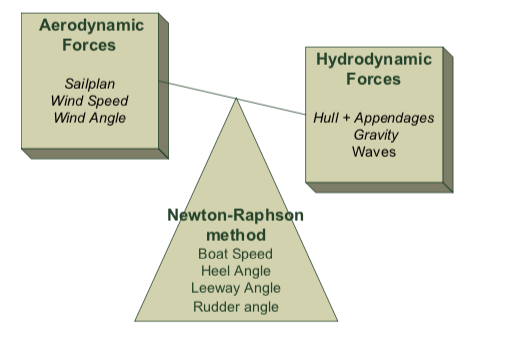
\includegraphics[width=0.5\hsize]{images/Vpp_balance_eq.png}
    \caption{VPP Force Balance Representation \cite{bohm2014velocity} }
    \label{fig:my_label}
\end{figure}
The VPP contains the solutions of the equations to accomplish this balance and it requires not only to solve the hydrodynamic and aerodynamic equations but also to know the properties of the sailboat related with its stability, such as $\lambda$ \cite{larsonprinciples}, \cite{milgram1998fluid}. The information required to get a VPP comes from different sources and all the variables involved can be classified in 4 categories or groups, according to \cite{philpott1993yacht} these groups are:
\begin{itemize}
    \item design (\textit{$_{d}$}): describe the size and shape of the sailboat and its elements.
    \item environment (\textit{$_{e}$}): describe the wind and current in which the sailboat will perform.
    \item control (\textit{$_{x_{c}}$}): these are setting variables that can be adjusted within some limits or constraints by the seamanship, such as $\beta_{r}$, $y_{c}$, \textit{f}, and \textit{r}.
    \item behavior (\textit{$_{y_{b}}$}): these variables describe the motion or condition of the motion at a given time or due to a given environmental condition. Examples of this type or variables are: $\lambda$, $\beta_{tw}$, $\Theta$, and the $V_{boat}$
\end{itemize}

\nomenclature[S]{$_{d}$}{Subscript for Design Variables}
\nomenclature[S]{$_{e}$}{Subscript for Environment Variables}
\nomenclature[S]{$x_{c}$}{Subscript for Control Variables}
\nomenclature[S]{$y_{b}$}{Subscript for Behavior Variables}
\nomenclature[S]{${aux}$}{Subscript for Auxiliary Variables}

The rest of the variables can be grouped as \textit{auxiliary} variables (\textit{$_{aux}$}). These variables describe transitional stages or intermediate calculations, such as $V_{aw}$, \textit{D}, \textit{L}, $M_{c}$, $M_{sail}$ among others. The arrangement of these groups results in at least 22 simultaneous nonlinear equations which can be solved by specifying a performance criterion and optimizing the \textit{$_{y_{b}}$} variables.
%From the equations of previous sections 18 variables were identiy as \textit{aux}.  
 
Because VPP plots are symmetric only half of it is usually represented as shown in figure \ref {typ_vpp}. The polar diagram indicates the wind direction or \textit{true wind angle} at 0\degree , $V_{boat}$ is defined by the radius size of the concentric half circles, the straight lines indicate the direction of the boat from the wind direction. Last, the wind speed is the group of lines that form a half heart shape; the intersection of these lines with direction lines indicates the maximum velocity that a sailboat can attain. \par 
\begin{figure} %[ht]
  \centering
  \subfloat[VPP plot for true wind angles from 0 \degree to 180\degree and true wind speeds from 4 to 10 m/s (7.77-19.44 kn) \cite{larsonprinciples}.]{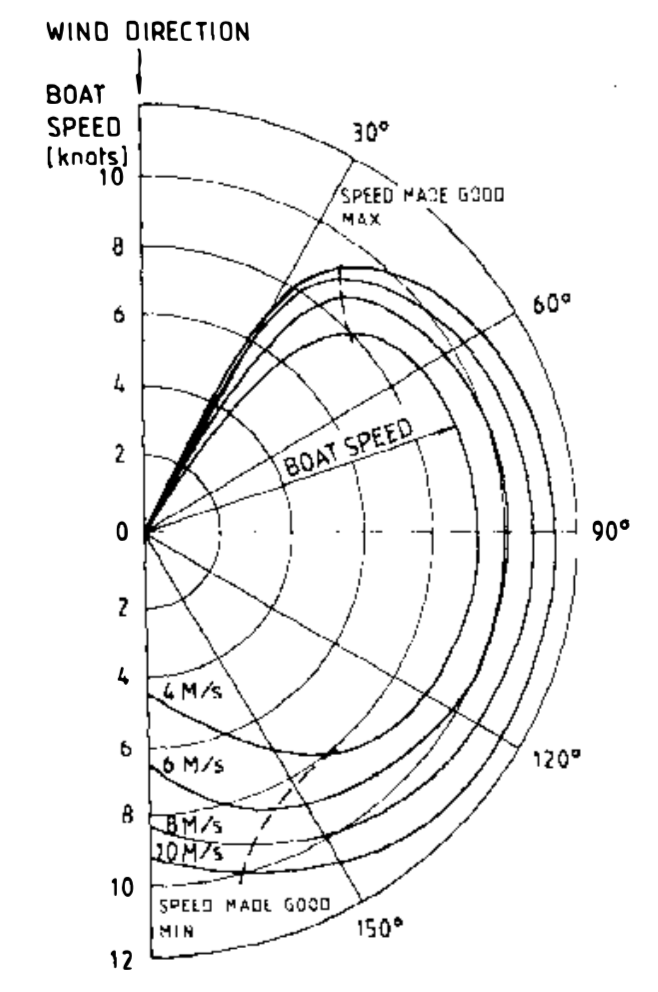
\includegraphics[width=0.38\linewidth]{vppLarsson1990.png}\label{typ_vpp}}
  \hfill
  \subfloat[Polar Curve of the Propulsion System \cite{yang2011control}(Full VPP representation).]{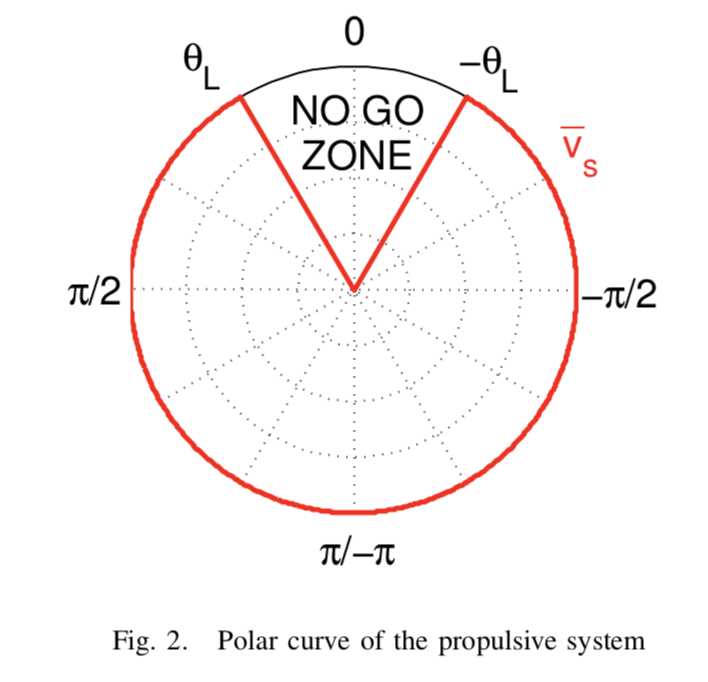
\includegraphics[width=0.45\hsize]{no-go_zone_yang.png}\label{no_go_zone}}
  \caption{VPP diagram}
\label{vpp_diag} 
\end{figure}

By using the VPP not only the direction of the maximum sailboat speed can be identified but also it shows the direction where the speed is the slowest. The angle range of this speed or speeds corresponds to the concave curve of the true wind, the area is defined as the \textit{no-go-zone} and it represents the set of directions that should be avoided to stay away from the irons \cite{yang2011control},\cite{denny2009float}, which means that under these directions the sailboat  motion is minimal, its propulsion is no enough or minimal to outweigh the resistance derived from the hull and sail.\par 

The performance criterion most used is to maximize $V_{boat}$ except when the sailing is towards the wind, upwind condition or sailing to windward. In this case, the performance criterion change from velocity to the distance that can be travel during a certain time.  This criterion is known as the velocity made good \textit{(VMG)} and it indicates where the sailboat is on the space from a reference and how is its motion \cite{larsonprinciples}, \cite{marchajaereo1979} \cite{philpott1993yacht}. \par 
\noindent
\textit{VMG} is determined by equation \ref{eq:VMG}. This relation can also be found in the velocity triangle, figure \ref{vel_triangle}, a more detailed geometrical is the figure \ref{fig:vmg_marchal_book}, where it is possible to identify how the $\beta_{tw}$ and $\lambda$ interact to gets the $\beta_{aw}$ therefore, how distance from the origin or reference point can be optimized and how different angles perform with the same given time. \par
\nomenclature[A]{$VMG$}{Velocity Made Good}

\begin{equation}\label{eq:VMG}
\begin{aligned}
VMG &=  \mid V_{boat} cos \beta_{tw} \mid 
\end{aligned}
\end {equation}

\begin{figure}
    \centering
    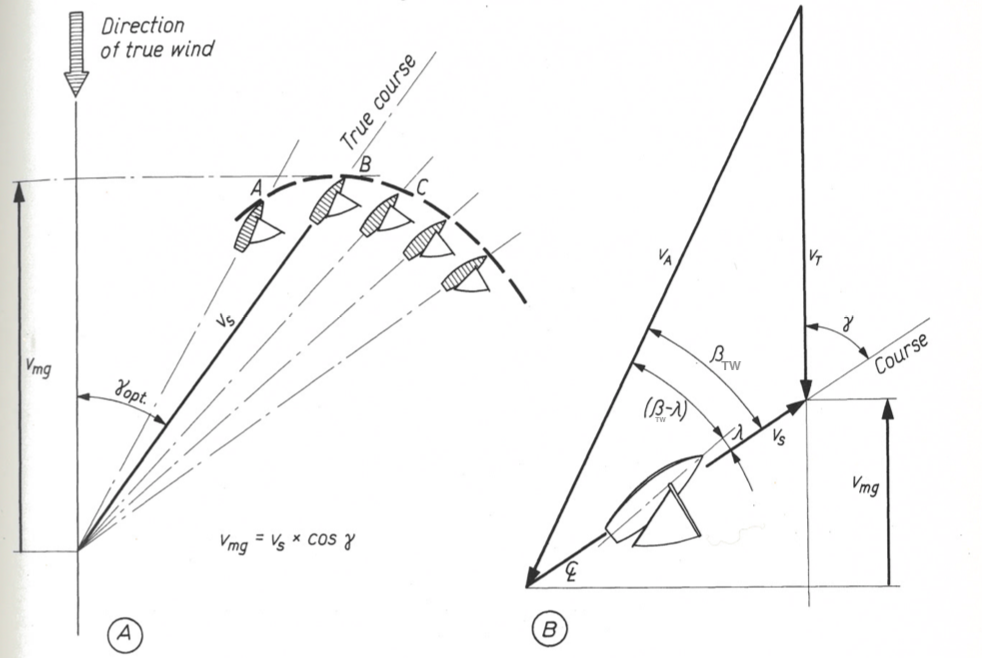
\includegraphics[width=0.75\linewidth]{vmg_marcha.png}
    \caption{Definition of VMG. A. VMG at  different angles. B. Velocity triangle including the leeway angle \cite{marchajaereo1979}.}
    \label{fig:vmg_marchal_book}
\end{figure}

The VPP is obtained by balancing the equations from previous sections, from equation \ref{eq:force_x} to equation \ref{eq:sail_moment}. It derives the $V_{boat}$ at different wind conditions and at different directions, angles respect to the wind. 

However, these equations are not usually solved in its six DOF. Because it was assumed that the vertical forces and moments are always in equilibrium, as was mentioned by \cite{larsonprinciples}, \cite{fossati2009aero} and on section \ref{sec:interaction_boat_environ}. The VPP partially solves the equations which means that the result provided only applies on 2D; particularly in the plane \textit{XY}. So it only considers the rolling moment and longitudinal forces  because changes on the \textit{Z} plane are neglected; but some of the variables related with the \textit{Z-axis} are considered, like $\Theta$. \par 
In this section, it was identified how the variables are categorized, most importantly which variables can be adjusted by the seamanship and which are defined by the sailboat and weather.


\section{Equations of Motion} \label{sec:eq_of_motion}
The motion of the boat from one point to another occurs in the XY plane. In the previous sections, the different components like forces generated by the wind and water were explained and how the seamanship or athlete compensate these forces by interacting with sailboat via sails,$\beta_{tw}$, and rudder, $\lambda$, mainly. On section \ref{section:forces_moment} 
it was mentioned that pitching moment and sway forces (vertical forces) are always in equilibrium, which means that heave and  pitch  motion can be omitted and the motion analysis only occurs on the XY plane within 4 DOF. These motions are the surge, sway, yaw, and roll.\par 

In 2004, de Keuning. et. al \cite{keuning2004mathematical} propose a mathematical model to describe the motion of sailboats or \textit{tacking maneuvers} with wide used parameters, like the information provided by the \textit{Delft Systematic Yacht Hull Series} (\textit{DSYHS}), so the estimation of the coefficients can be defined from this model without the need for experimental data for specific sailboat. \par 

\nomenclature[A]{$DSYHS$}{Delft Systematic Yacht Hull Series}

In the model, the main change refers to its coordinate system, figure \ref{fig:csys_tackmodel} shows the that the coordinate system is at the center of the sailboat, the \textit{Z-axis} is positive orientation when it points downwards and the \textit{Y-axis} is pointing at starboard \cite{keuning2004mathematical}. \par

\begin{figure} %[ht]
  \centering
  \subfloat[Motion depict by the mathematical model.]{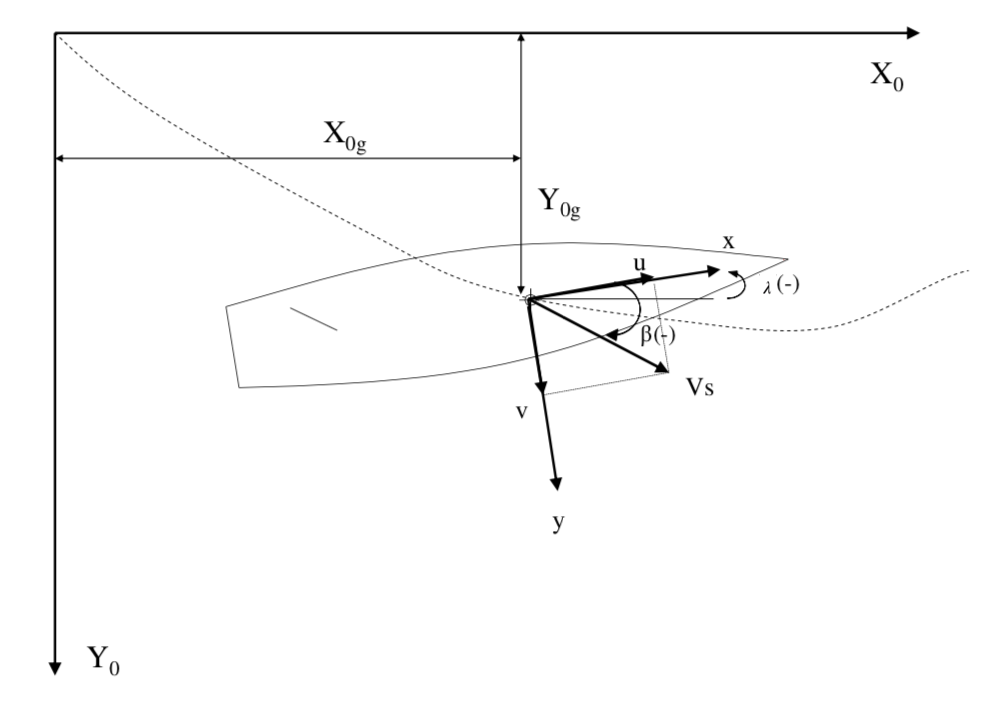
\includegraphics[width=0.38\linewidth]{ridder_motion.png}\label{fig:motion_csys_tackmodel}}
  \hfill
  \subfloat[Angle's location and axis orientation according to the coordinate system.]{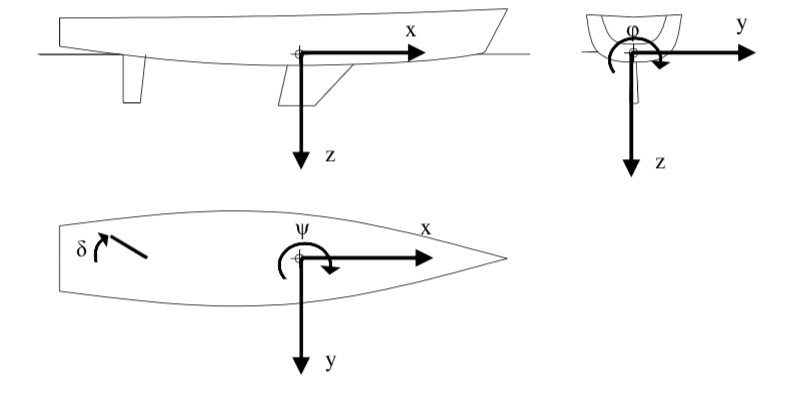
\includegraphics[width=0.45\hsize]{ridder_caxis.png}\label{fig:axis_cystackmodel}}
  \caption{Motion depiction of the mathematical model bestow by the coordinate system \cite{keuning2004mathematical}.}
\label{fig:csys_tackmodel} 
\end{figure}

The next equations or Euler's equations for sailboats motion described by \cite{keuning2004mathematical} define the total forces applied in the sailboat element corresponded to the main axis.\par

\nomenclature[S]{$X_{U}$}{Hull resistance in the upright position on the X direction}
\nomenclature[S]{$X_{i}$}{Forces in X direction of the \textit{i} element}
\nomenclature[S]{$Y_{i}$}{Forces in Y direction of the \textit{i} element}
\nomenclature[S]{u}{Velocity along the X direction}
\nomenclature[S]{v}{Velocity along the Y direction}
\nomenclature[S]{$\Dot{u}$}{Acceleration in the X direction}
\nomenclature[S]{$\Dot{v}$}{Acceleration in the Y direction}

The forces on the X and Y axis are: \\  
\begin{equation}\label{eq:force_X_motion}
    X_{U}+X_{hull}+X_{rudder}+X_{sail}=m_{T}(\Dot{u}-v\Dot{\psi})
\end{equation}
\begin{equation}\label{eq:force_Y_motion}
    Y_{hull}+X_{rudder}+X_{sail}=m_{T}(\Dot{v}-u\Dot{\psi})
\end{equation}
And the momentum on the X and Y axis are: \\
\begin{equation}\label{eq:moment_X_motion}
    K_{hull}+K_{rudder}+K_{sail}+K_{stability}=I_{xx} \Ddot{\phi}
\end{equation}
\begin{equation}\label{eq:moment_Y_motion}
    N_{hull}+N_{rudder}+N_{sail}=I_{zz} \Ddot{\psi}
\end{equation}
%<vertical forces are in balance always same as the pitching moment
where: 
\begin{itemize}  \label{symbols o motions}
 \setlength \itemsep{0em}
\item $m_{T}$ = the total mass of the sailboat not including crew.
\item u = velocity along the X-axis.
\item v= velocity along the Y-axis.
\item $\phi$ = roll angle, related to $\Theta$.
\item $\psi$ = yaw angle. %which is the course angle respect to the wind).
\item $I_{xx}$ = total mass moment of inertia in the roll axis (X.axis).
\item $I_{zz}$ = total mass moment of inertia in yaw axis (Z-axis).
\item K = Rolling moment (X-axis).
\item N = Yawing moment (Z-axis).
\item $X_{U}$ = is the hull resistance in the upright position.
%\item $X/Y_{hull}$ = is the resistance of the hull under the heeled resistance.
\end{itemize}

\nomenclature[S]{$m$}{Total mass of the sailboat including crew mass}
\nomenclature[S]{$K_{i}$}{Rolling moment (X-axis) of the \textit{i} element}
\nomenclature[S]{$N_{i}$}{Yawing moment (Y-axis) of the \textit{i} element}
\nomenclature[S]{$I_{ii}$}{Total mass moment of inertia in the \textit{i-axis}}

It is important to clarify that $\psi$ and $\phi$ are variables that describe the location of the sailboat over an area while and they are related with $\Theta$ and $\lambda$ from the kinematics of the sailboat; because the motion described by Keuning et. al \cite{keuning2004mathematical} includes waves effect because of this there is a difference between $\phi$ and $\Theta$. The heel angle $\Theta$ is the rotation from the \textit{Z} plane in \textit{flat water}; while $\phi$, the roll angle, is $\Theta$ plus the rotation induced by the fluctuations on the front wave \cite{kimball2009physics}, \cite{denny2009float}. \par 
\textit{ $ K_{stability} $ } is the moment generated by the weight when $\Theta$ is not zero; the center of buoyancy (\textit{B}) of the sailboat moves laterally and when its vertical line crosses the midplane of the sailboat creates a metacenter (\textit{M}). The distance between \textit{CG} and \textit{M} is known as the metacentric height, \textit{$\overline{GM}$} ) \cite{patterson2014ship} this displacement generates an oscillation and a mass moment that is calculated as follow:
\begin{equation} \label{eq:k_stability}
    K_{stability}=-mg\overline{GM} sin \phi 
\end{equation}

\nomenclature[A]{$B$}{Center of buoyancy}
\nomenclature[A]{$M$}{Metacenter}
\nomenclature[S]{$\overline{GM}$}{Metacentric Height}
\nomenclature[A]{$CG$}{Center of Gravity}

The rudder and the sail are sailboat elements controlled by the seamanship. 
The rudder produces hydrodynamic forces and momentum, as explained in section \ref{sec:momentum_types}; and the weight of the crew generates a momentum \ref{eq:Moment_crew} 
this momentum can be included on the previous equations by assuming that the centroid of $W_{c}$ is located in the center of gravity (\textit{CG}) and so forth the equations are:\par

Surge  (X-axis):
\begin{multline}\label{eq:force_xMasuyama}
    X_{U}+X_{hull}+X_{rudder}+X_{sail}+X_{V\Dot{\psi}}V\Dot{\psi}\\ =(m+m_{x})\Dot{u}-(m+m_{y}cos^2\phi+m_{z}sin^2\phi)v\Dot{\psi}
\end{multline}
\\
Sway  (Y-axis):
\begin{multline}
\label{eq:force_yMasuyama}
Y_{hull} + Y_{rudder} + Y_{sail} + Y_{\Dot{\phi}} \Dot{\phi} + Y_{\Dot{\psi}} \Dot{\psi} \\ 
=\{(m + m_{y})cos^2 \phi + m_{z} sin^2 \phi \} \Dot{v} + (m + m_{x})u \Dot{\psi} + 2(m_{z} - m_{y}) sin\phi cos\phi \cdot v \Dot{\phi}
\end{multline}
\\
Roll (X-axis):
\begin{multline}
     K_{hull} + K_{rudder} + K_{sail} + K_{stability} +K_{\Dot{\phi}} \Dot{\phi} \\
 =(I_{xx} + J_{xx}) \Ddot{\phi} - {(I_{yy} + J_{yy})-(I_{zz} + J_{zz})} sin\phi cos\phi \cdot \Dot{\psi}^2
\end{multline}  \label{eq:m_xMasuyama}
\newline
Yaw (Z-axis):
\begin{multline}
   N_{hull}+N_{rudder}+N_{sail}+N_{\Dot{\psi}}\Dot{\psi}\\
 = \{ (I_{yy} + J_{yy}) sin^2 \phi +(I_{zz} + J_{zz})cos^2 \phi \} \Ddot{\psi} +2 \{(I_{yy} + J_{yy})-(I_{zz} + J_{zz})\}sin\phi cos\phi \cdot \Dot{\psi} \Dot{\phi}  
\end{multline}\label{eq:m_yMasuyama}
\newline
where: 
\begin{itemize}  \label{symbols_motions2}
 \setlength \itemsep{0em}
\item m = mass of the boat without crew
\item $m_{i}$ = the added masses in \textit{i} direction.
\item $I_{ii}$ = total mass moment of inertia.
\item $J_{ii}$ = total added mass moments of inertia.
\begin{itemize}
    \item i= x,y and z.
\end{itemize} 
\item $X_{V\Dot{\psi}}$, $Y_{\Dot{\psi}}$, $N_{\Dot{\psi}}$  = hydrodynamic derivatives of the hull due to yawing.
\item $N_{\Dot{\phi}}$, $K_{\Dot{\phi}}$  = hydrodynamic derivatives of the hull due to rolling.
\end{itemize}

\nomenclature[S]{$J_{ii}$}{Total add mass moment of inertia in the \textit{i} direction }
\nomenclature[S]{$\Dot{\psi}$}{Angular Velocity in the yaw axis (\textit{Z-axis})}
\nomenclature[S]{$\Dot{\phi}$}{Angular Velocity in the roll axis (\textit{X-axis})}
\nomenclature[S]{$\Ddot{\phi}$}{Angular Acceleration in the roll axis (\textit{X-axis})}
\nomenclature[S]{$\Ddot{\psi}$}{Angular Acceleration in the yaw axis (\textit{Z-axis})}
\nomenclature[S]{$X_{V\Dot{\psi}}$, $Y_{\Dot{\psi}}$, $N_{\Dot{\psi}}$}{Hydrodynamic derivatives of the hull due to yawing motion}
\nomenclature[S]{$N_{\Dot{\phi}}$, $K_{\Dot{\phi}}$}{Hydrodynamic derivatives due to rolling}

By using the last equations it is possible to determine the position of the boat and because the sailboat to model is the \textit{dinghy}, sailed by \textit{professional athletes}, the heel angle is considered small close to 0 ( \textbf{$\Theta \approx$ 0}). This assumption means: \textbf{$X_{hull}$, $Y_{hull}$, some terms of $M_{hull}$ and $M_{sail}$ will be canceled, and the \textit{yaw equation} can be neglected}. The \textit{yaw equation} not only because of the restriction of one boat design but because the athletes keep the balance on this axis; additionally, competitions are regulated in such way that the safety of the participants is not compromised, this last restrict the $V_{boat}$. \par 

With this assumptions the equations of motion can be simplified as: \\
Surge  (x axis):
\begin{equation}
       X_{U}+X_{rudder}+X_{sail}+X_{V\Dot{\psi}}V\Dot{\psi}  =(m+m_{x})\Dot{u}-(m+m_{y})v\Dot{\psi}
\end{equation}\label{eq:Fx_motion}
Sway  (y axis):\par 
\begin{equation}
\label{eq:Fy_motion}
Y_{rudder} + Y_{sail} + Y_{\Dot{\phi}} \Dot{\phi} + Y_{\Dot{\psi}} \Dot{\psi} 
=(m + m_{y})\Dot{v}  + (m + m_{x})u \Dot{\psi}
\end{equation}
\\
These 2 equations can be reorganized so we can get the accelerations vector of the sailboat. The only decision variable identifies until know refers to $\Dot{\psi}$, which is related to the \acrshort{b_aw}%$\beta_{aw}$
, therefore, the $\lambda$. 
From the equation of section \ref{section:forces_moment} and substituting in equation \ref{eq:Fx_motion} and in \ref{eq:Fy_motion} the previous equations becomes:
\begin{equation}\label{eq:X_tot}
    X_{TOT}=X_{U}+X_{rudder}+X_{sail}
\end{equation}
\begin{equation}\label{eq:X_tot2}
    X_{TOT}=Rcos\psi+F_{R}cos\psi+Scos\psi+
    %-\frac{1}{2}\rho_{w}V_{ac}^2 C_{D,h} +F_{l,r}sin \beta_{ac}-F_{d,r}cos \beta{ac} + F_{l,s}sin \beta_{aw} - F_{d,s}cos \beta_{aw}
\end{equation}
\begin{equation}\label{eq:y_tot}
    Y_{TOT}=Y_{rudder}+Y_{sail}
\end{equation}
\begin{equation}
    Y_{TOT}=F_{R}sin\psi+S sin\psi
    %-F_{l,r} cos \beta_{ac} - F_{d,r}sin \beta_{ac} -F_{l,s}cos\beta_{aw}-F_{d,s}sin \beta_{aw}
\end{equation}

\begin{equation}\label{eq:u_dot}
    \Dot{u}=\frac{X_{TOT}}{m+m_{x}}+v\frac{m+m_{y}}{m+m_{x}} \Dot{\psi}+\frac{X_{V\Dot{\psi}}}{m+m_{x}}V\Dot{\psi}
\end{equation}
\begin{equation}\label{v_dot}
    \Dot{v}=\frac{Y_{TOT}}{m+m_{y}}-u\frac{m+m_{x}}{m+m_{y}} \Dot{\psi}+ \frac{Y_{\Dot{\psi}}}{m+m_{y}}\Dot{\psi}
\end{equation}
\begin{equation}\label{x_dot}
    \Dot{x}=ucos\psi +u_{tw}+u_{tc}
\end{equation}
\begin{equation}\label{y_dot}
    \Dot{y}=usin\psi +v_{tw}+v_{tc}
\end{equation}
where:
\begin{itemize}
    \item $u_{tc}$ = True current velocity in the \textit{X-axis}
    \item $v_{tc}$ = True current velocity in the \textit{Y-axis}
\end{itemize}
From table \ref{table:SNAME_notation} it was defined that $\psi$ is related with \textit(r) the yaw angular velocity, and it defines the position or orientation of the boat, which means that it set the direction of the course ($\lambda$).  $\lambda$ is considered a behavior variable(\textit{$y_{b}$}) in section \ref{sec:VPP}. % it was mentioned 
%that  . One of this variables is $\lambda$,  %one of this variables is $\beta_{r}$ while one of the behaviour variables that describes motion is $\lambda$, 
Because it describes the motion of the sailboat, and the seamanship set the direction, this variable is set as a control variable.\par

This chapter explained how the motion of a sailboat can be determined in 2D with the different types of variables or sources for information. In the next chapter, the environmental variables \textit{e} are going to be explained and how they interact with the equations of this chapter.
%\chapter{Integrating the Weather Model into the Sailing Path Generation}
% Question to answers during the next chapters
%%% Instruments used, set-up, materials
%%Description of the instruments and materials

\chapter{The Weather Research and Forecasting Model(WRF) in the Sailing Path Generation} \label{ch:weatherModel} 

%Introduction
The wind model used in this research is a numerical weather prediction (\acrshort{nwp}) known as the Weather Research and Forecasting Model (\acrshort{wrf}). This particular model has the ability to forecast weather and serves as a tool for atmospheric research. This chapter explains the characteristics of the common weather forecast provided during and before the Olympic sailing races and compare it with the requirements of athletes and coaches. This comparison shows the importance of a customized weather(wind) model and describes its characteristics and limitations. \par \noindent 

For the purpose of this project, the model provided is a \acrshort{wrf} wind model stored in a NetCDF file, while the measured data from past race events is provided in a tabular layout. The last part of the chapter explains the reference frames and their relation with the sailboat velocity.\par

The importance of the wind is not only because it is considered the main propulsion source of the sailboat; but also, because it is the wind which demands changes to the seamanship, like direction on the rudder and sail, to balance the kinematic equations of chapter \ref{ch:physics_sailboat}, and reach the maximum velocity  estimated by the \acrshort{vpp}.In such manner, the seamanship uses the wind information to maximize the velocity of the sailboat by adjusting the direction of the sailboat in a similar way the algorithm for path generation uses that information. \par

\nomenclature[A]{NWP}{Numerical Weather Prediction}
\nomenclature[A]{WRF}{Weather Research and Forecasting Model}

\section{The application of the weather models into Olympic Sailing Races} \label{sec:WindModel_on_Olympics}
%WRF weather models into Olympic sailing races}

A wind model forecast is based on a 3-dimensional time-space model, which can be described as a 4-dimensional model. The resolution of this model or granularity is defined by the size of the data sets that describe it. Moreover, the use of weather models during the summer Olympic Games is not new, but neither widely used. In sailing, the main use of them is as an informative source for the organizers. It helps to warranty the safety of the competitors, like in the Para-Olympic events, and reduce delays due to the wind conditions of the competition  \cite{spark2004wind}, \cite{sheng2009structure}, \cite{golding2014forecasting}. Only \cite{giannaros2018ultrahigh} refers to the \acrshort{nwp} model as a tool to develop a strategic plan to course the race for a sailing team. \par 

Previous to competing, athletes and coaches know the exact location of the sailing area which is enclosed by a diameter of a magnitude between 0.8 and 1.5 nm (1.482 - 2.778 km) and course diagrams \cite{SailRaceRio}. For them, it is important to identify wind patterns, such as average magnitude, direction, the range of variation, the location of vortexes, and even the time of the day when they occur. This information allows coaches and athletes to develop a strategic plan to course the race by avoiding undesirable conditions or to maximize the use of favorable zones.\par

Even when the location, dates and times of the races are known, the wind characteristic and details about the area is still not well understood. The time horizons of local forecasts of short term know as \textit{nowcast} for public access is between 1 to 2 hours as a minimum and up to 6 hours, with a spatial resolution between 40 to 100 km \cite{warner2010numerical}, \cite{kristensen2010weather}. These local predictions use measurements from weather stations or any weather data available around the area of interest and extrapolate in time these conditions; whereas days or weekly forecast can use deterministic predictions.\par

Because sailing Olympic races are set into a grid of 2km with a maximum duration of 1 hour; the public information about wind (weather forecast) does not meet the requirements of the athletes and coaches. As a consequence, customized models have been developed to provide the information required by them. A clear example of this type of models was developed by Giannaros \cite{giannaros2018ultrahigh}, which is defined as a \acrshort{wrf} with \textit{ultrahigh resolution wind forecasting}.\par 

An ultrahigh resolution, a detailed level of granularity, means that the spatial variation captured by the model is in the order of hundred meters in the horizontal plane. In this case, the minimum grid size used was about 200 meters on the area of interest and surrounded by different grid sizes up to 25 km. The vertical dimension was defined by 40 unequally spaced elevations or altitudes; while the duration of the forecast stands for 48 hours starting at 0:00 UTC hours each day with a time interval or time step of 30 minutes. \par \noindent 

Just considering the area of the course which is placed within a grid of 2 km, a model of ultrahigh resolution has a granularity of 10,200 data sets or 39.5$\times 10^6$ data points. The model developed by Giannaros has more data sets since the \acrshort{nwp} model considers a larger area around the races and other factors which will be explained in the next section. Furthermore, it was calculated using 300 computer cores of a high-performance computing cluster and more than 900,000 core hours \cite{giannaros2018ultrahigh}. 

Before \cite{giannaros2018ultrahigh}, only \cite{philpott2001optimising} and \cite{allsopp2000optimal} developed models to include the weather for offshore yacht competitions. Instead of using an \acrshort{nwp} model to determine the wind, each work uses a different stochastic process to calculate it. The details about the discretization of the time were not provided. Only \cite{philpott2001optimising} acknowledged a short-course competition where the Markov process only applied to the wind direction; the granularity of the model was 4000 data sets with a time step of 5 seconds. Other applications of wind models refer to vessels routing where the focus is on fuel costs and other logistics metrics. \par 

The \acrshort{wrf} model can provide the detailed information required by the sailors and coaches of Olympics Classes; however, it demands time and high-performance computing equipment, without considering the preliminary input data and validation process it requires to have a feasible and reliable model to work with. In the other hand, the inclusion of weather models for path generation has not evaluated the sensibility of the trajectory due to the granularity of the model. The next section will provide the details about the \acrshort{wrf} model used for this project as well as its general characteristics. \par 

\section{Components of the WRF Wind Model} \label{sec:WRF_WindM}
Weather models, like wind or current models, are discretized over the space and time because the data is organized into a four-dimensional grid data sets. The most used computer formats to share this type of models are GRIB(.grib) and NETCDF(.nc). The form in which they organize the information may differ but both formats contain the volume representation of the wind model. A straightforward format sometimes used to share the information is the tabular format with all the variables as headers. \par

%\subsection{The WRF Model }
The \acrshort{wrf} is a model that combines global atmospheric models with regional measurements to developed high-resolution models. This means that regional models are inserted within global models, as a result, its range of applications is from meters to many latitude-longitude degrees. The integration allows the identification of small climate variations and other types of phenomena, like precipitations. The incorporation of observable data measured at a constant rate and at known locations given flexibility to the model and unification of the available data \cite{warner2010numerical}. \par

\subsection{Spatial Representation of the Wind Model} \label{sec:Space_WindM}

Weather models are volume representations of a particular region, because of this, it is important to identify the data dimensions, to either manipulate or extract properly the variable of interest, like the wind velocity, if the height does not match the CE of the sail, equation \ref{eq:wind_h} should be used to determine it. \par \noindent

Figure \ref{fig:map_projection} shows the sketches of the most common type of map projection used on atmospheric modeling. The main idea of these projections is that a set of rays coming from the same axis of rotation project points from the sphere into the surface of projection which later can be flattened. The advantage of them is that the angles between curves are preserved and the distance distortions are the same in all directions of a point. The map projection to use depends basically on the latitude of interest \cite{warner2010numerical}. \par

\begin{figure}
    \centering
    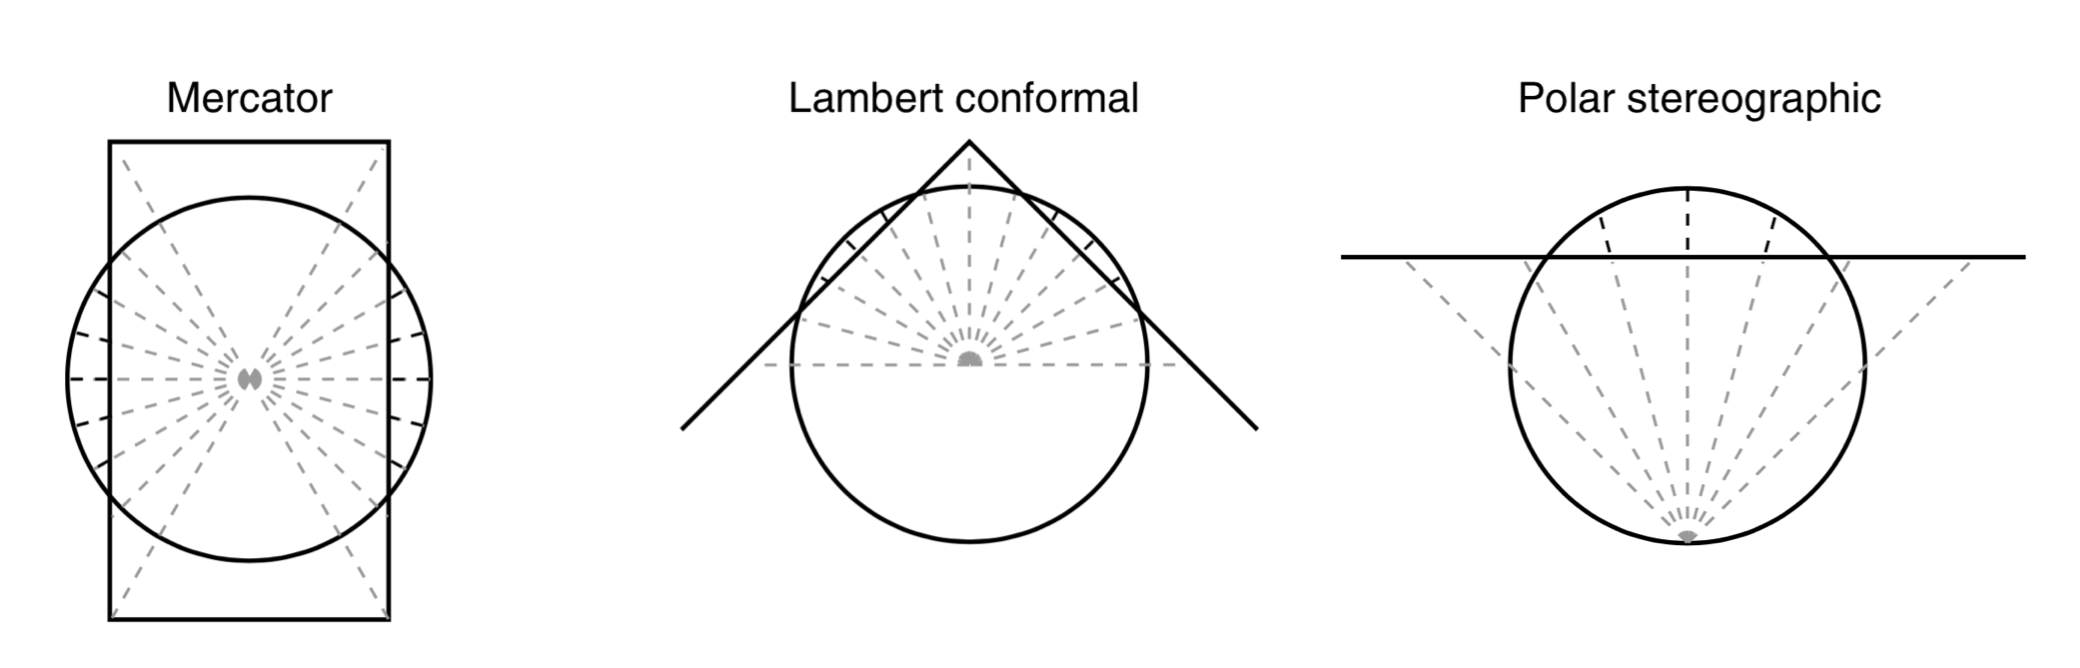
\includegraphics[width=1 \linewidth]{map_proj.png}
    \caption{Most common map projections used on atmospheric models. Mercator is a cylinder projection commonly used for grids in tropical latitudes, Lambert-conformal is a cone, used for mid-latitude grids and the Polar stereographic uses a plane and is used for high latitude grids. The axis of all 3 is always coincident with the Earth's axis. \cite{warner2010numerical}.}
    \label{fig:map_projection}
\end{figure}

The points on the spatial grid of the \acrshort{wrf} model are quasi-regular because the grid is defined by the map projection used. Each intersection of the grid is a data point defined by 4 dimensions (\textit{$n(x_{i},y_{j},z_{k},t)$}) and it represents the location of a variable value. The value of $\Delta x$ is chosen to have a sufficient number of grid points to adequately represent the smallest meteorological feature of interest. \par

Under some circumstances, the model uses a nested approach; where $\Delta x$ is reduced as it gets close to the area of interest. The size of the grid was a crucial concern for \cite{giannaros2018ultrahigh} since the topography of public databases were replaced by new sets that at least match the size of the stipulated grid.\par

\subsection{Time Representation on the Wind Model}\label{sec:Time_onWindM}
The time dimension on the forecast models is limited by the \textit{Courant number} and in consequence with the spatial resolution required. Modifications on the grid have implications closely related with the computational effort; since on each time step the space equations on each grids point have to be solved. The measurement data is another element to incorporate and related to time. \par 

The computational effort for weather models results from the space granularity. Meanwhile, the time step brings stability to the model. Then a small time step provides stable solutions to the equations. While the computational effort is related to the space granularity in a non-linear form. For example, if only one space dimension is double (by a factor of 2), the computational effort time will be 8 times more. \par 

The use of measurement data has an impact on the quality of the results because the rate of their incorporation and values adjust the model forecast. Figure \ref{fig:data_meas_integration} shows how often the measured data is incorporated into the model. This incorporation determines the rate of the re-initialize and the number of cycles within the model forecast that it has to assimilate the observable values. In this form, the measured data not only affects the time of processing but also the accuracy of the forecast. \par

\begin{figure}
    \centering
    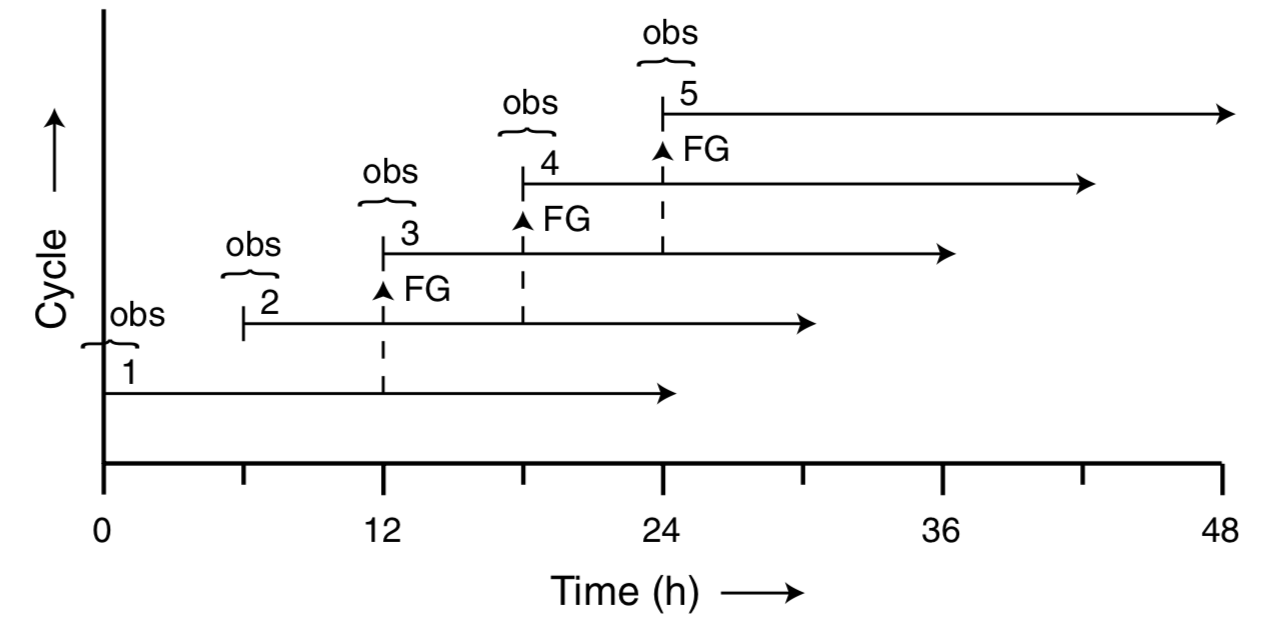
\includegraphics[width=1 \linewidth]{re-run_model.png}
    \caption{Forecast Model with the integration of measured data. During 24 hours, the forecast models are adjusted every 6 hr by the observations. This generates 4 cycles which are assimilated by the model \cite{warner2010numerical}. }
    \label{fig:data_meas_integration}
\end{figure}

\section{The WRF model for the World Cup Series 2018 Hyéres, France}\label{sec:WRF_WindM_FR}

The algorithm for the minimal time path for sailing competitions was developed considering the characteristics of the \acrshort{wrf} wind model on a date of competitions so wind measurements are available. The measurements served not only to set-up the model but also to compare their results. Since \cite{giannaros2018ultrahigh} found that the topography allocation and representation in addition to the initialization of the model have a great impact on the results. \par

The World Cup Series 2018 Hyéres, France Laser competition was chosen. The area where the races took place was named as Charly and the coordinates of its center were: 43\degree 02.869'N, 006\degree 13.221' E. The diameter of the area was 1.6 nm (2.96 km). The date was April 24, 2018. The model forecast 24 hours starting at 0:00 Hrs local time and it was provided by professor Sukanta Basu from the Geoscience Department at TU Delft. \par 

The information of the wind model was stored in the NetCDF file which is organized in dimensions, variables and attributes defined as data sets \cite{netcdf56302}. In this case, 4 coordinates describe the location and time of the wind velocity. The attributes vector refer to the dimensions of each variable, in this case, the velocity's units were $m \backslash s $. \par 

The wind speed variables were \textit{u} and \textit{v} velocities. Over a rectangle area of coordinates: 41.663\degree N, 4.752\degree E and 7.251\degree N, 44.451\degree E. The grid size is about 1 km or approx 0.009\degree. The coordinates latitude and longitude where store independently and discretize over a plane of 198$\times$300 elements. \par

The components of the wind velocity were stored on a grid plane of 199$\times$300 for \textit{u} and 198$\times$301 for \textit{v} velocity. This arrangement is known as grid staggering where the different dependent variables are on different grids so the spatial resolution is increasing while the effects of truncation error are decreased. The velocity corresponding to each coordinate is the horizontal average velocity calculated as equations \ref{eq:hor_AVG_velu} and \ref{eq:hor_AVG_velv} indicate.  \par  

\begin{equation} \label{eq:hor_AVG_velu}
    u_{{i,j}_{avg}}=\frac{ u_{i,j} + u_{{i+1},j} } {2}
\end{equation}

\begin{equation} \label{eq:hor_AVG_velv}
    v_{{i,j}_{avg}}=\frac{ v_{i,j} + v_{i,{j+1}} } {2}
\end{equation}

The vertical dimension, height, of the model where discretized over 50 non-uniform steps. The first level corresponds to 7.8 m while the second height is at 25 m. Because the \acrshort{ce} is estimated to be at 2.68 m from the water level \cite{pennanen2015optimal} and the measurements were taken at 10 m above the sea level, equation \ref{eq:wind_h} is used to determine the \acrshort{kappa} value and convert \acrshort{u} and \acrshort{v} fields to the corresponding height. Finally, \acrshort{v_tw} and \acrshort{b_tw} on each grid point can be calculated with equations \ref{eq:v_tw} and \ref{eq:b_tw}, respectively. \par \noindent Equation \ref{eq:b_tw} uses the four-quadrant inverse tangent, (atan2(Y,X)) from \acrshort{matlab} to return values over the [$- \pi, \pi  $] interval.\par 

\begin{equation}\label{eq:v_tw}
    V_{tw_{i,j}}=\sqrt{{u_{i,j}}^2+{v_{i,j}}^2}
\end{equation}

\begin{equation}\label{eq:b_tw}
    \beta_{tw_{i,j}}= atan2d \frac {v_{i,j}}{u_{i,j}}
\end{equation}

The 24 hrs forecast model was discretized in time steps of 10 minutes or ${1} \backslash {6}$ hr. This means that there are 145 steps on the time dimension. Figure \ref{fig:wind_model_FR} shows the wind model provided at 2 different hours, the difference of time is only 1 hour and 10 minutes. The red cross is the center of laser course area named Charly and the black arrows indicate the direction of the wind. The figure also shows the relevance on the scale or granularity; on one side public forecast weather are larger than the one showed here; in the other hand, the interested region is too small even when the granularity was increased significantly. \par    

\begin{figure} [hb!]
  \centering
  \subfloat[Wind model forecast at 10:00 Hrs]{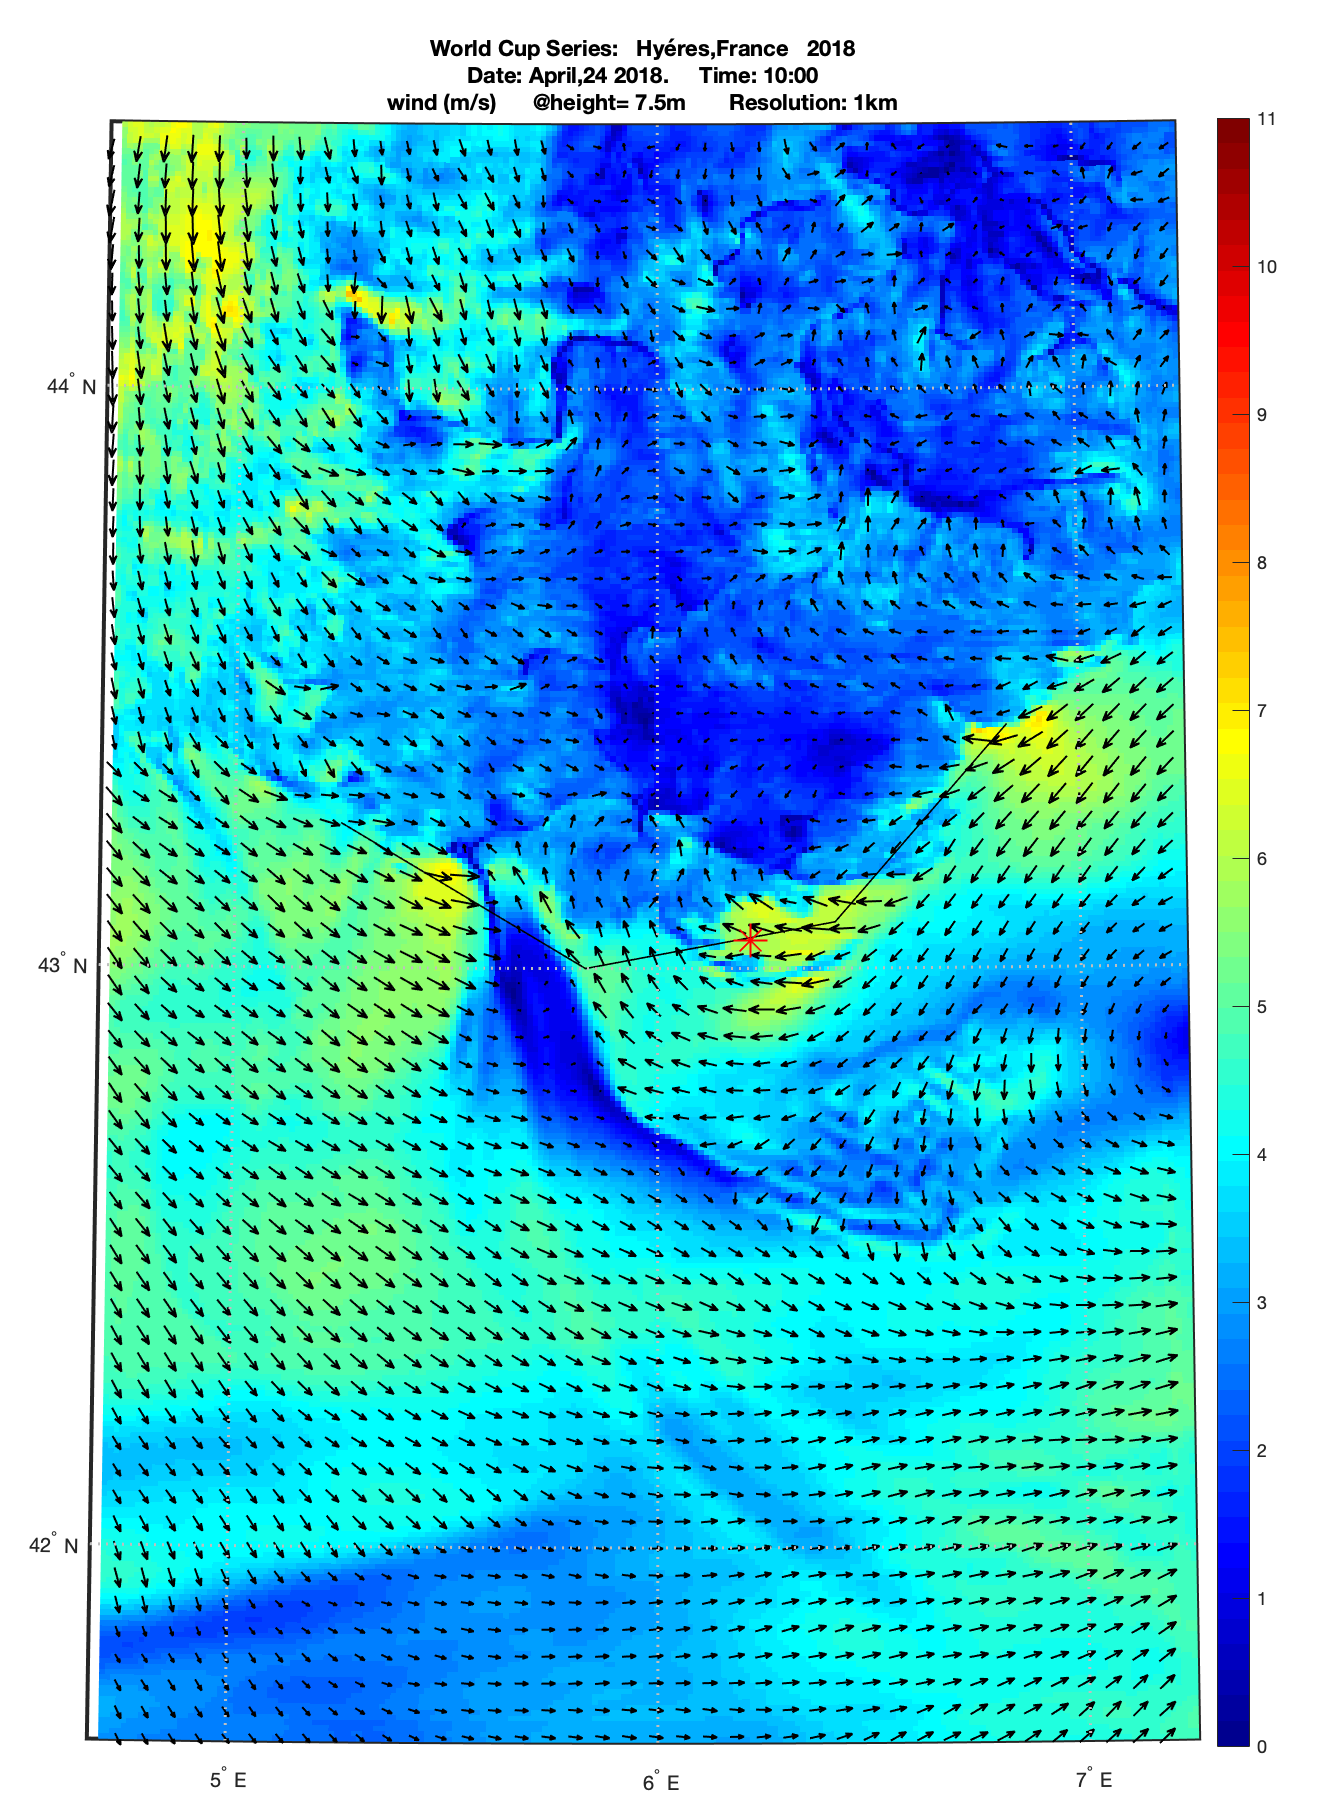
\includegraphics[width=0.5\hsize]{images/fr_10_22.png}\label{fig:fr_10hr}}
  \subfloat[Wind model forecast at 11:10 Hrs]{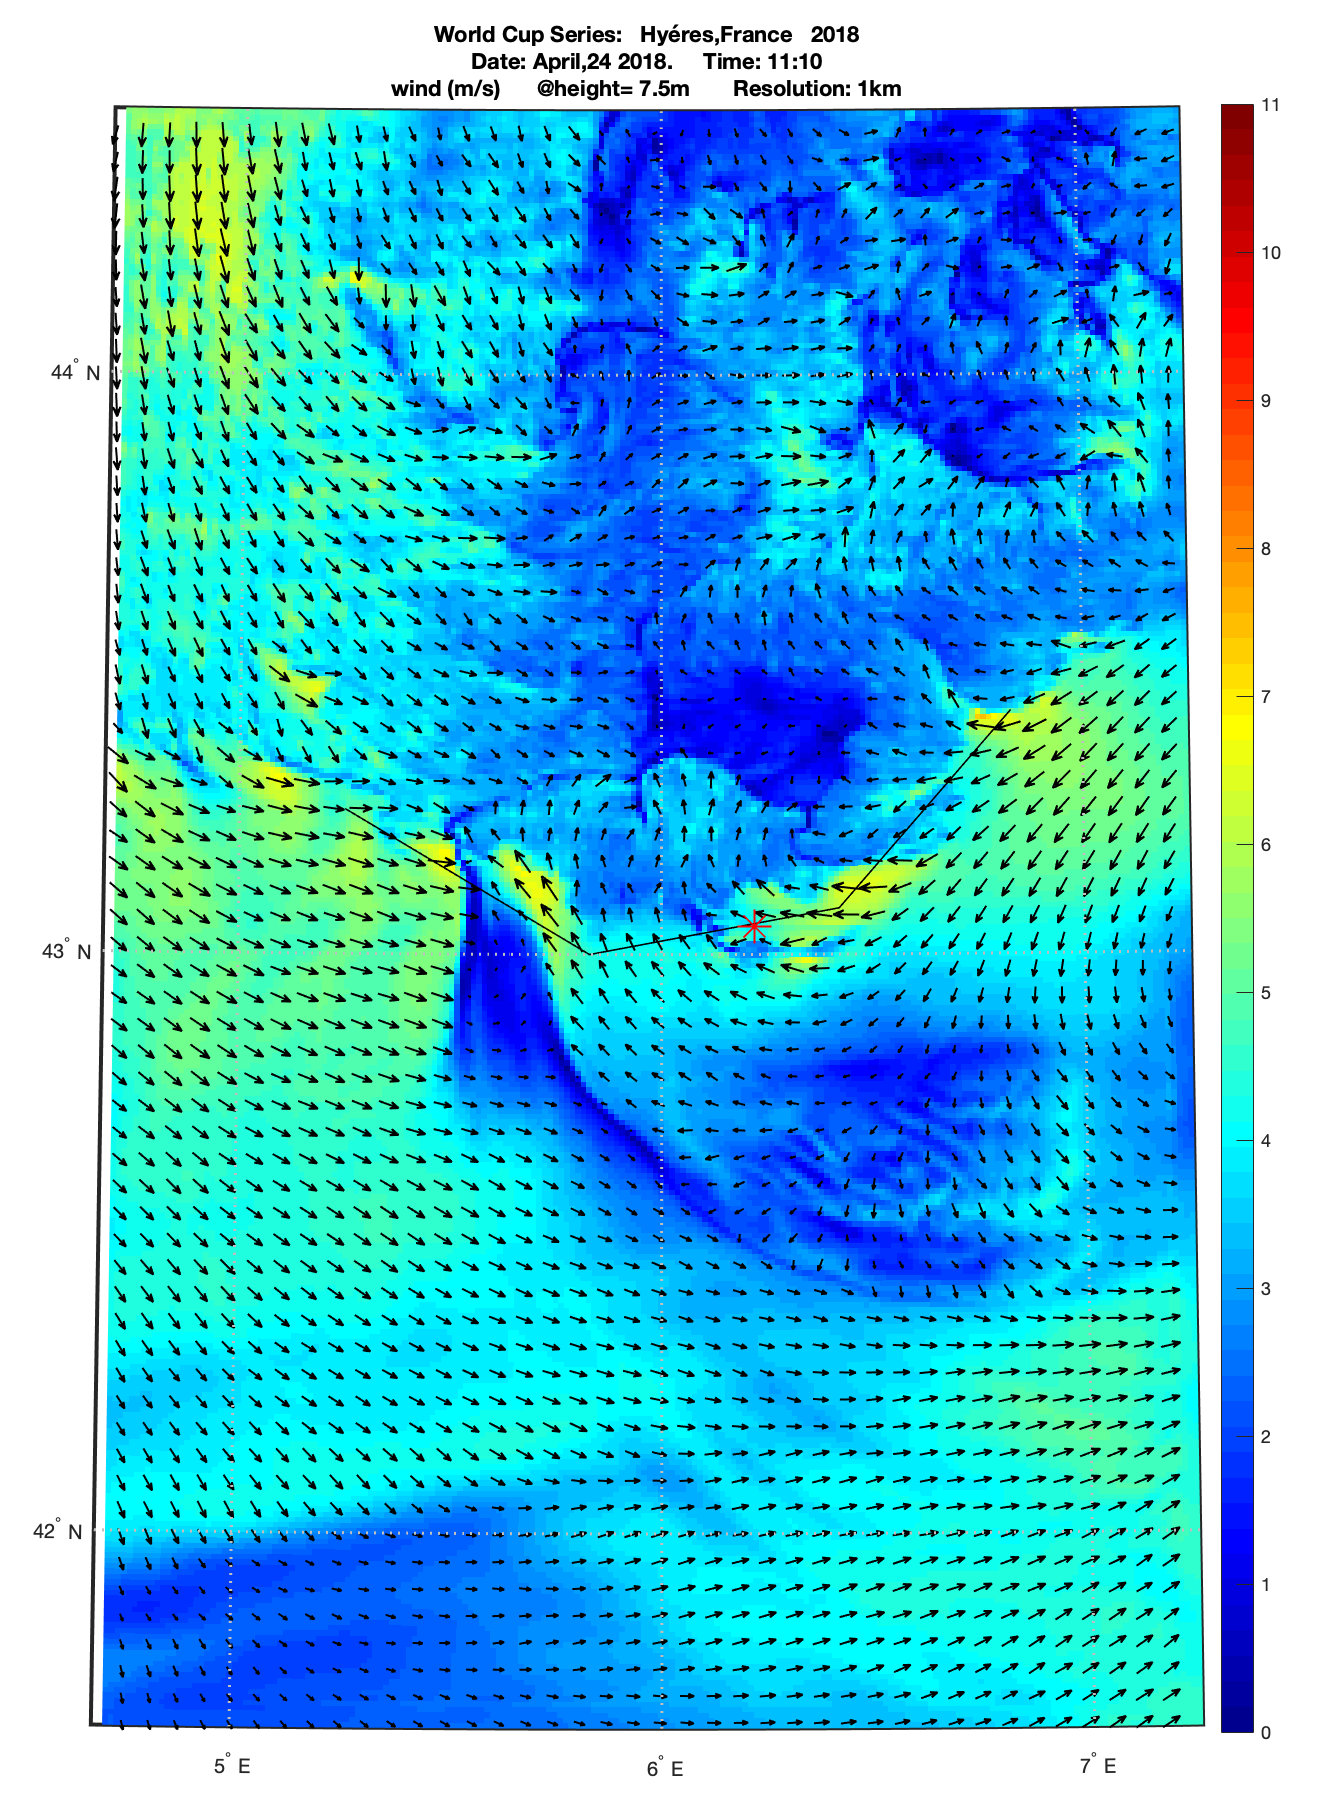
\includegraphics[width=0.5\hsize]{images/fr_11_22.png}\label{fig:fr_11hr}}
  \caption{Wind Model for the World Cup Series 2018 at Hyéres, France. The red asterisk indicated the center of the Charly area for the Laser Course. The area of the model is defined by the corner coordinates at 41.663\degree N, 4.752\degree E and 7.251\degree N, 44.451\degree E.}
\label{fig:wind_model_FR} 
\end{figure}
In summary, the wind model provided is a 4D(\textit{(x,y,z,t)}) grid model of 198 $\times$ 301 $\times$ 50 $\times$ 145 datasets with a space resolution ($\Delta x$) of 1 km and time step ($\Delta t$) of 10 minutes(600 seconds). This kind of granularity is defined as high resolution, and despite the size of the grid the area of competition, its center looks small. This is one of the reasons why \cite{giannaros2018ultrahigh} developed a model with ultrahigh space resolution.\par  

\section{Reference Frames the relation between wind and sailboat velocities} \label{sec:RefFrames}

The wind velocity and direction determines the velocity of the sailboat. However, the wind velocity perceived by the seamanship when the sailboat moves is not the same as the velocity of the sailboat. This perceived velocity is known as the \textit{apparent wind} (\acrshort{v_aw}) and it not only includes the velocity and direction of the wind but also the velocity and direction of the current (\acrshort{v_tc} and \acrshort{b_tc}). The \acrshort{v_aw} and \acrshort{b_aw} are not new concepts, they were introduced on section \ref{sec:wind_vel_trian} and on equation \ref{eq:vel_appVector}. \par

The \acrshort{v_aw} is modified by the current in a similar form as on equation \ref{eq:vel_appVector}, from this equation the current vector is subtracted as shown in equation \ref{eq:vel_wind_current} this velocity is defined as \acrshort{v_awc}. The vector expression shows how different directions influence the results even when the magnitude is the same. On the other hand, if the boat is moving in the same direction as the wind then the apparent velocity increases \cite{denny2009float},\cite{allsopp1998stochastic}. \par 

\begin{equation} \label{eq:vel_wind_current}
\vv{V_{a_{w,c}}}= \vv{V_{tw}} -\vv{V_{tc}} - \vv{V_{boat}}
\end{equation}

However, the previous equation is not the only modification to consider related to wind. %The wind model describes the velocity of the wind 
The wind model only applies over a specific region on the Earth-fixed frame, while the sailboat frame moves along it and is located as indicated by section \ref{sec:eq_of_motion}. It was assumed that the area and the trajectory of the sailboat can be expressed as [\textit{X,Y}] coordinates. This is possible for Olympic Sailing Races because the course area is relative small compared with the total surface of the Earth. Thus to convert the latitude-longitude to [\textit{X, Y}] coordinates, the \acrshort{matlab} function \textit{deg2utm(Lat, Lon)} can be used \cite{allsopp1998stochastic}.\par \noindent 

For the purposes of this research, it is assumed that the Earth circumference is about 40003.2 km. In addition, the nautical mile is one minute (\textit{$1 \backslash 60 \degree$}) of arc on the surface of this sphere, thus the nautical miles is 1852 m. \par 
   
\begin{figure}[hbt!]
    \centering
    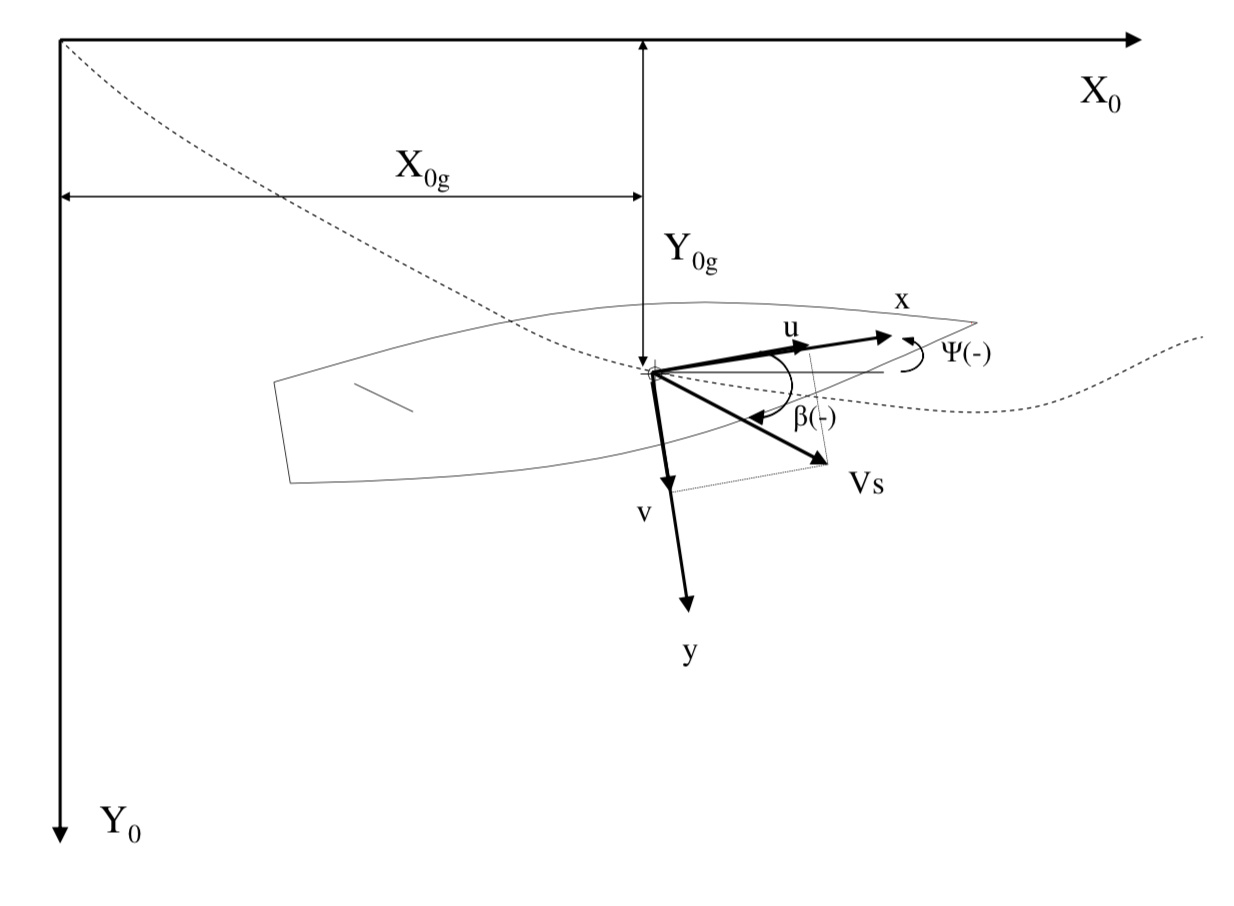
\includegraphics[width=.8 \hsize]{boat_csys.png}
    \caption{Sailboat reference coordinate system and Earth-fixed reference frame \cite{keuning2004mathematical}. }
    \label{fig:boat_Csys}
\end{figure}

Since the sailboat displaces through the horizontal plane of the wind model, another transformation has to be applied in order to describe the motion and forces of the sailboat. Figure \ref{fig:boat_Csys} shows how \acrshort{u} is always aligned with the sailboat mid-plane, therefore to its heading direction (-$\Psi$). The change in orientation respect to the same reference frame is done with the rotation matrix \ref{eq:RotMat}. This transformation is shown in equation \ref{eq:velTransFrame} and it expresses the velocity from the Earth-fixed frame to the sailboat-fixed frame \acrshort{v_btw} \cite{yang2011control}, \cite{bohm2014velocity}, \cite{Alves2014ASailboat}, \cite{keuning2004mathematical}.\par 
\begin{equation}\label{eq:velTransFrame}
    V_{tw}^b= \mathcal{R} \cdot V_{tw}= \mathcal{R}
    \begin{bmatrix}
    u\\
    v
    \end{bmatrix}
\end{equation}

\begin{equation} \label{eq:RotMat}
    \mathcal{R}(- \Psi)=
    \begin{bmatrix}
    cos \Psi & sin\Psi \\
    -sin \Psi & cos \Psi
    \end{bmatrix}
\end{equation}

If the \acrshort{v_tc} is included in the model without waving effects the \acrshort{v_tw} has to be modified before the transformation of equation \ref{eq:velTransFrame}. This is expressed in equation \ref{eq:V_twModifV_C} \cite{allsopp1998stochastic}. However, more equations like the \acrshort{b_aw} and \acrshort{v_aw} have to be redefined because of this inclusion. The equations modified are shown next:\par

\begin{equation}\label{eq:V_twModifV_C}
    \vv{V_{tw,c}}=\vv{V_{tw}}- \vv{V_{tc}}
\end{equation}

\begin{equation}\label{eq:v_twCurBoat}
    V_{tw,c}^b=\mathcal{R} \cdot V_{tw,c}
\end{equation}

\begin{equation} \label{eq:VelCurrWind_boat}
    \vv{V_{aw,c}^b}= \vv{V_{tw,c}^b} - \vv{V_{boat}}
\end{equation}

\begin{equation}\label{eq:b_tw_c}
    \beta_{aw,c}= atan2d \frac {v_{aw,c}^b}{u_{aw,c}^b}
\end{equation}

The transformation of the terms from the sailboat-fixed to the Earth-fixed coordinate system and \acrshort{v_tw} using \acrshort{RM} is not necessary on the equations from \ref{sec:eq_of_motion} since they were already included in their development \cite{keuning2004mathematical}.\par  

\nomenclature[A]{$ MATLAB\textsuperscript {\textregistered}$}{MATLAB R2018b Student License}

\nomenclature[S]{$V_{tc}$}{True Current Velocity}
\nomenclature[S]{$\beta_{tc}$}{True Current Angle}

\nomenclature[S]{$V_{a_{w,c}}$}{Apparent Velocity due to wind and current}
\nomenclature[S]{$V_{tw}^b$}{True Wind Velocity respect to the sailboat}
\nomenclature[S]{$\mathcal{R}$}{Rotational Matrix}
\nomenclature[S]{$\Psi$}{Heading Direction of the sailboat over the horizontal plane}
\nomenclature[S]{$V_{tw}^b$}{True Wind Velocity respect to the sailboat}
\nomenclature[S]{$V_{tw,c}$}{True Wind Velocity affected by true current velocity($V_{tc}$)}
\nomenclature[S]{$V_{tw,c}^b$}{True Wind Velocity affected by $V_{tc}$ respect to the sailboat}
\nomenclature[S]{$V_{aw,v}^b$}{Apparent Wind Velocity affected by $V_{tc}$ respect to the sailboat}

This section explained the \acrshort{wrf} wind model used for the generation of trajectories on Olympic Sailing Races. The characteristics of this model define some of the parameters of the Path Algorithm, therefore for the Minimal Time trajectory. The scale of the Olympic Sailing Courses is small compared with the coverage of wind models, the impact of this coverage hasn't been evaluated and the use of customized models is very limited. Even when the algorithm to develop does not include any model for current, and it is assume that current velocity \acrshort{v_tc} is constant some modifications have to take place. 
% Question to answers during the next chapters
%%% Instruments used, set-up, materials
%%Description of the instruments and materials
%%How the instruments are set-up and what auxiliary connections might need to be used.
%%% add statment
\chapter{Algorithm to Optimize the Sailing Path for Laser Classes.} \label{sec:AlgOptSail}
%Introduction
The optimization problem for the minimal path is a problem frequently related with logistics and operations research. This type of problem is usually related with the \textit{Euclidean} shortest path and solved either with networking optimization or dynamic programming (\textit{\acrshort{dp}}). Although for Olympic sailing classes the optimal path is not related with distance but with time instead. \par \noindent 
Because of this, the research of this type of problem on sports is limited and it is mainly focused on yacht competitions. Whereas the laser class is the smallest and one of the most used sailboats on Olympic Classes. The objective of this section is not only to explain widely used methods but their elements and how they should apply to develop and algorithm for the Laser Olympic class.\par

Many techniques used on \acrshort{dp} and networking optimization can be used in combination with the \acrshort{vmg} criterion to developed and optimization algorithm for laser races.  Because the target's location and the geometrical domain are the features that allows the used of both criteria thus the optimal solution is found inside the polygon \cite{mitchell2000geometric}.\par 

The first part of this chapter explains how chapter \ref{ch:physics_sailboat} and chapter \ref{ch:weatherModel} are integrated to develop the algorithm to optimized the path of laser boats and obtain a minimal time path. But because most of the formulas on section \ref{sec:equil_equat} are generic, the adjustments required to describe the laser class are explained in the second part of this chapter. Followed by the explanation about the algorithm, details such as the objective function, the constraints and its validation. The validation of the algorithm is at the end of the chapter, and it provides information about the parameters defined by the user and at the initialization of the algorithm. \par 

%\section{Incorporation of the Wind Model into a Path Algorithm}
\section{Weather Routing Models and Path Algorithms for Sailboats}\label{sec:weatherRoute}

Uncertainty weather is a typical condition that not only yacht competitions have to manage but also maritime transportation. The direction-dependency of the vessel's velocity is seen as a series of regions where the flow's velocity is designed as uniform. This is characterizes as an anisotropic medium condition, and path algorithm problems with this characteristic has been solved with different methods \cite{dolinskaya2013fastest}. \par 
\noindent 
The most used methods related with vessels or yachts and anisotropic medium come from operations research and logistics. For example, from operations research these methods are dynamic programming (\acrshort{dp}), direct and indirect methods while the networking method is related with logistics. \cite{kelly2015transcription},\cite{mitchell2000geometric}. In the networking method the order in which the locations can be reach is not as important than time. \par 
The formulation of the problem is focus on the time and not in the length of the trajectory. However, it is the velocity of the sailboat the one that determines the direction of the sailboat and considers the wind properties. Because of this, equation \ref{eq:rabaudmintime} defines the time of the path to displace a sailboat between 2 points \cite{rabaudoptimal}. This is the easiest formulation of the problem but it shows how this problem differs from the shortest path approach.  \par

\begin{equation} \label{eq:rabaudmintime}
\begin{aligned}
T_{AB}=\int_{A}^{B} dt=\int_{A}^{B} \frac{dl}{v}  \\
\end{aligned}
\end{equation}

\subsection{Dynamic Programming and direction-dependence for Path Algorithms} \label{sec:dynProg}

\acrshort{dp} is a widely used technique to solve the optimal path problem for yachts and maritime transportation. The reason is because it breaks the main problem into multiple stages all connected. In this case, to move from point \textit{A} to point \textit{B} the trajectory is conformed for more than two points. Meaning that the main trajectory is conformed by multiple stages or smaller trajectories continuously coupled until it arrives to its final destination. \par \noindent 
The fact that one stage depends on the previous one, allows the recognition of the state of the variables implicated in that solution. This set of state variables is used to optimize the trajectory by iterating each stage until the optimal solution by stage is found. Thus the next stage always start from the optimal solution given by the last stage \cite{philpott2001optimising}. \par

In yacht competitions and maritime transportation, the trajectory is not only defined by the location of the points but also by the area within they are located. This area has to be defined first and later discretized not only to use variables that depends on its location and time, like wind and current, but also to apply \acrshort{dp}. The discretized area is composed by nodes and the line that connects 2 nodes is defined as an arc ($c_{arc}$). For example, node \textit{i} and \textit{j} is connected by the $c_{arc}(\textit{i,j,t(i)})$ which also depends on time (\textit{t}). Since the time at the starting point(\textit{$t_{A}$}) and the wind (\textbf{w}\textit{(i,j,t)}) and current(\textbf{c}\textit{(i,j,t)})  characteristics are known, the minimal time path using \acrshort{dp} is defined in equation \ref{eq:DP_minTimeP_Allsop}  \cite{zyczkowski2017method},\cite{allsopp2000optimal}.

\begin{equation} \label{eq:DP_minTimeP_Allsop}
f^*(i,t)=
\begin{cases}
0,  &  \\
\\
\noindent 
\displaystyle
\min_{j \in \Gamma_{i}} \Bigg[c_{arc}(i,j,t)+f^*\Big(j,t + c_{arc}(i,j,t)\Big) \Bigg]\\
\end{cases}
\end{equation}
\hspace{20mm} otherwise
\begin{equation}
j^*(i,t)=
\noindent 
\displaystyle
arg \min_{j \in \Gamma_{i}} \Bigg[ c_{arc}(i,j,t)+f^*\Big(j,t + c_{arc}(i,j,t)\Big) \Bigg], \quad i \neq n_{finish} 
\end{equation}

The equation explains how the time is minimized at each node until the final destination,point \textit{B}, is reached. $f^*$\textit{(i,t)} is the time at node (\textit{i,t}) which is optimal time resulting from the previous stages. $j^*$\textit{(i,t)} is the next node from \textit{i} on the optimal path, while $\Gamma_{i}$ is the set of subsequent nodes of \textit{i}. The minimal time of equation \ref{eq:DP_minTimeP_Allsop} to move from node \textit{i} at time \textit{t} when the next node is \textit{j} is given by:\par 
\begin{equation*}
    c_{arc}(i,j,t)+f^*\Big(j,t + c_{arc}(i,j,t)\Big) 
\end{equation*}

\noindent
Figure \ref{fig:dp_Allsop} is the graphical explanation of the equation to determine the minimal time from node 1 to 5, starting at time 1 (\textit{n(1,1)}). Node 5 ($n_{5}$) can be reach by 3 different paths, or in other words, there are 3 alternative nodes before $n_{5}$ can be reach.  The nodes 2, 3 and 4 can be reach at different times, the minimum time between them is given by $n_{4}$ with a time of 2 (\textit{n(4,2)}). The next arc is formed from $n_{4}$ to $n_{5}$ and because the starting time of $n_{4}$ is the minimal/optimal time for the first stage, the final time is then the minimum time path from $n_{1}$ to $n_{5}$. \par \noindent
These state-space algorithm for the shortest path includes explicitly the time dimension \cite{allsopp1998stochastic}.

\begin{figure}[hbt!]
    \centering
    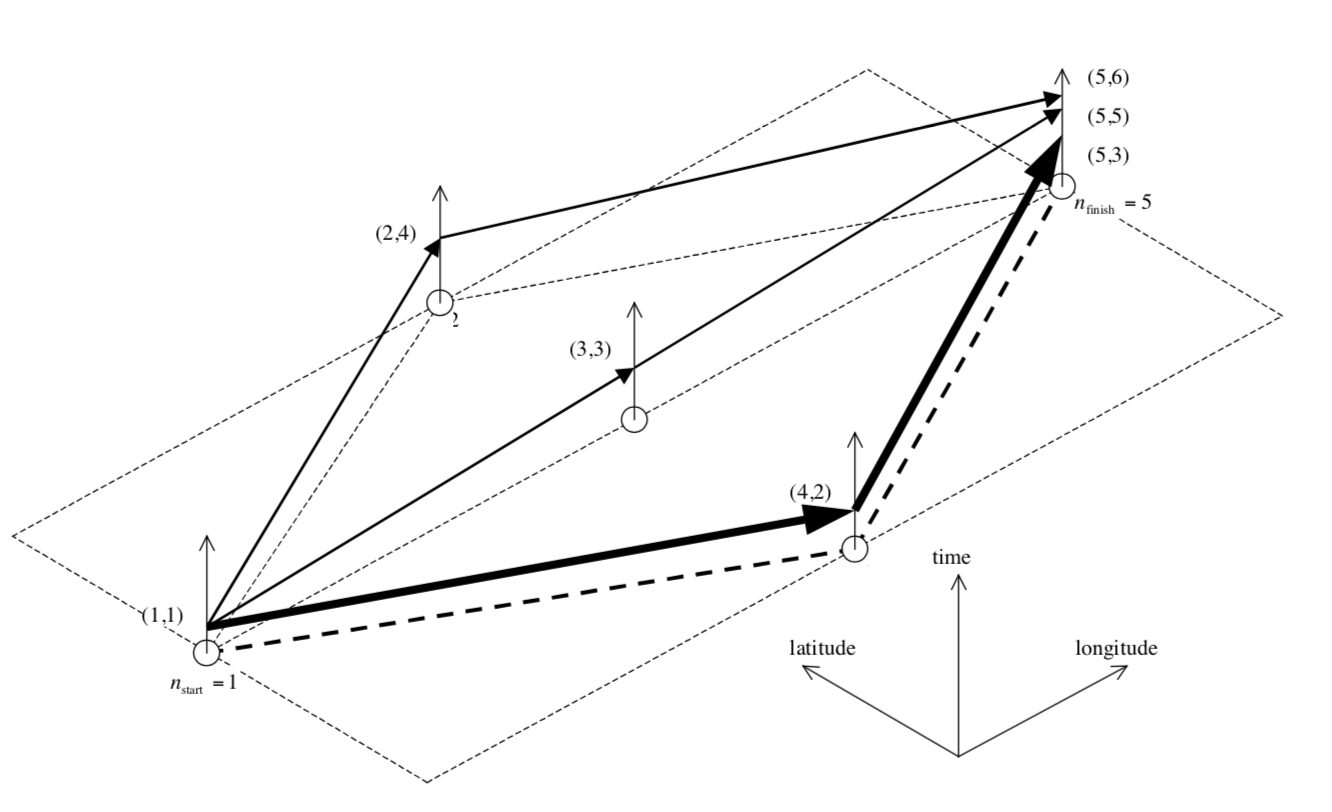
\includegraphics[width=.85 \linewidth ]{Allsopp1.png}
    \caption{Minimal Time Path from node 1 at time 1 (\textit{n(i,t)=n(1,1)}) to node 5 using \acrshort{dp}. The minimal time path to move from node 1 to 5 has go through node 4 and the path is indicated by the thicker  line \cite{allsopp2000optimal}.}
    \label{fig:dp_Allsop}
\end{figure}
\par 

An alternative process to discretize the area is based on the grid method and the heading decision, which is driven by the maximum velocity of the sailboat. This method can be related with the \acrshort{vmg} criterion because the same distance from the starting point can be reached at different times. Here, the heading-angle decision is discretized by intervals of size $\Delta \Psi$, clockwise and counterclockwise as a result multiple sub-routes are generated. If the symmetry of the \acrshort{vpp} is taken into account, some nodes and sub-routes can be represented within a diamond shape \cite{xing2012path} \cite{zyczkowski2017method}. \par \noindent
The number of stages($n_{stages}$) along the straight sailing distance (\textit{L}) between point $P_{0}$ and $P_{n}$ determines the shortest distance between (\textit{L} $\backslash n_{stages}$ ). In this case $n_{stages}$ can have any value bigger than 1 and it can be seen as the number of attacks that the seamanship could perform. The bigger the number the longer the time of the computational effort to determine the trajectory of the optimal time path \cite{xing2012path}. \par 
\noindent
The optimal heading is finding when the next stage is reached at the minimal time. In this case it is possible that multiple nodes arrive at the same time to the next stage. For this reason, the sub-routes have to been stored and the process continues until the destination point is reached. The algorithm to estimate the minimal time path is similar to the $c_{arc}$ process, the difference is in the from in which the area and stages is determined. The heading-direction approach sometimes uses additional factors over directions where the speed is the maximum. \par

Figure \ref{fig:diamondshape_subR} shows how the heading decision works. In this particular case, e all the sub-routes from $P_{0}$ to $P_{n}$ are contained into a diamond shape. Each node is describe by the stage and the node-number per stage, $P n_{stage},i_{sub-route}$ which is determined by the size of $\Delta \Psi$. The nodes over the edges of can only reach the half of nodes compared with the nodes at the center. The number of clear stages represented here are 6 and on each node there a maximum number of sub-routes is 21 and a minimum of 10. It is importance to remember here the concept of the \textit{no-go-zone} from section \ref{sec:VPP} because it could reduce the range of the heading direction angle.\par 

%\begin{figure}[hbt!]
%\centering
%  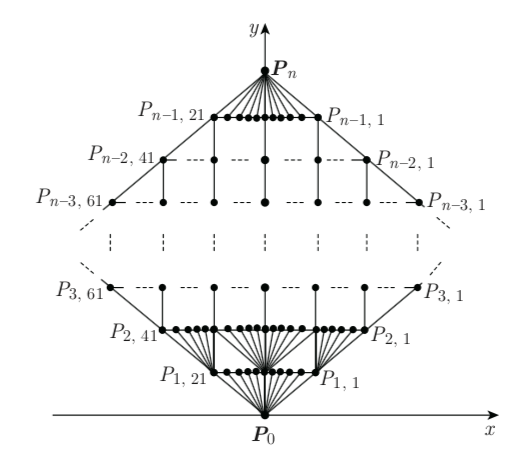
\includegraphics[width=0.6\linewidth]{legyachtxing.png}
% \caption{Leg yatching model \cite{xing2012path} }
%\label{fig:xing_nodesi}
%\end{figure}

\begin{figure} [hbt!]
  \centering
  \subfloat[Sailing Area Discretization for a Sailing Path from point A to B \cite{zyczkowski2017method}.]
  {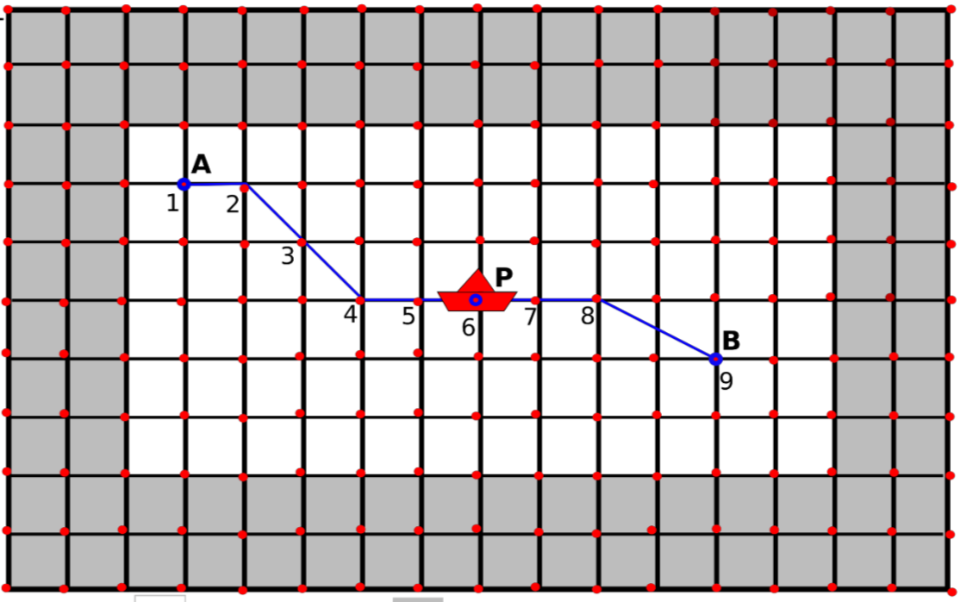
\includegraphics[width=0.33 \linewidth]
  {Sailing_area_heading.png}\label{fig:GridAreaSail}}
  \hfill 
  \subfloat[Heading Directions at a node, 8 angle discretizations \cite{zyczkowski2017method}.]{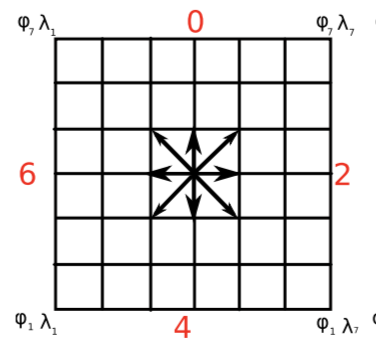
\includegraphics[width=0.22\hsize]
  {HeadDirNode.png} \label{fig:HeadAngle_Discret}}
  \hfill
  \subfloat[Diamond Shape with the Sub-routes for a heading-angle discretization to move from $P_{0}$ to $P_{n}$ \cite{xing2012path}.]
  {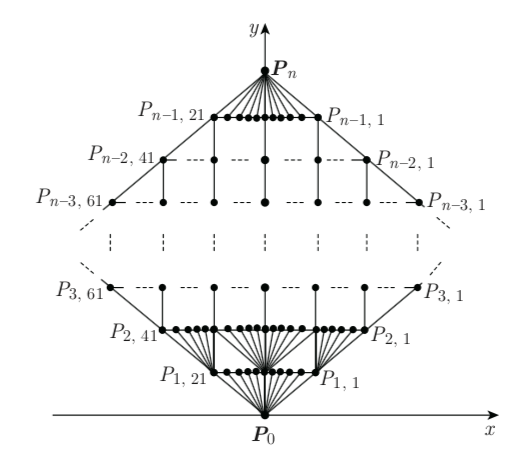
\includegraphics[width=0.33 \linewidth]{legyachtxing.png}
  \label{fig:diamondshape_subR}}
  \caption{Area discretized with a sailing path and Heading Angle discretization}
\label{fig:AreaDiscret} 
\end{figure}

\subsection{Path Algorithm Using Isochrones} \label{sec:isochrones}
A common solution with visual information obtained with \acrshort{dp} in weather routing are the isochrones. The isochrones lines compose a map where each line shows the maximum distance a sailboat can reach during a certain time. Moreover, this map can be seen as the visual representation of the \acrshort{vpp} over different anisotropic media when the weather variation is minimal \cite{allsopp1998stochastic}. \par 
A similar approach relates this type of solution with geometrical optics more specific with wavefronts. This analogy is because the speed of the wavefront depends on the refractive index of the material \cite{rabaudoptimal}.Figure \ref{fig:isochrone_ex} shows how the \textit{qtVlm} software uses isochrones to determine the optimal path for a generic yacht.\par

\begin{figure}[hbt!]
    \centering
    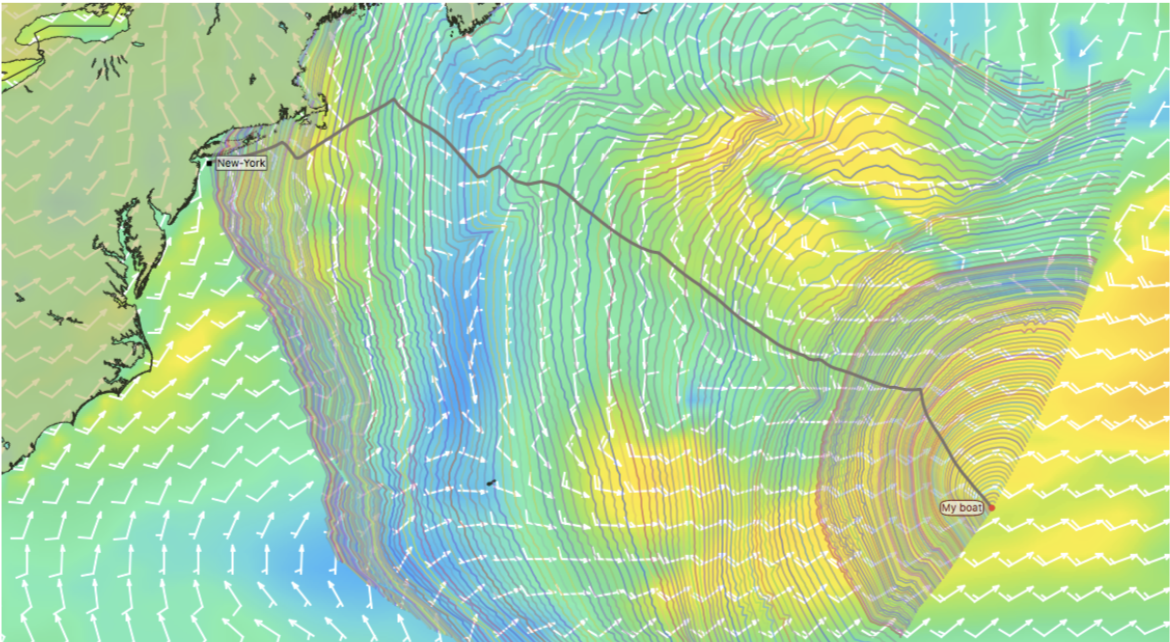
\includegraphics[width=.75 \linewidth]{isochrone_ex.png}
    \caption{Optimal Path Solution from qtVLm software using isochrones for a generic Yacht from a random location over the Atlantic to New York. The optimal path is the gray thick line, the wind direction is indicate by the white arrows.. The \cite{rabaudoptimal}. }
    \label{fig:isochrone_ex}
\end{figure}

The visual information presented by most these algorithms has been employed by various weather routing software. Despite of this, the use of them in sports and in Olympic Sailing Classes is limited. This because they are designed for long-distance yachts races or for maritime-logistics purposes. In both cases, the weather model is assumed to be homogeneous in space and time and frequently loaded from public sources. Meaning that the time step and grid size is much bigger than the required for Olympic Sailing races. Furthermore, when it is used for maritime-logistics purposes the vessels are equipped with communication and other measured systems that accounts for weather variations. \par
Despite the advantages of the isochrones techniques and its usage on large course races, the number of application for short courses is limited. The reason is because the weather is assumed to be perfectly known and even when the \acrshort{vpp} is assumed symmetric the algorithm doesn't explain or shows the limitations of choosing the symmetric path not even as an alternative for some space-time-intervals.\par    

%The envelop shape of the VPP used in \cite{rabaudoptimal} was explained in detail by \cite{dolinskaya2009optimal}.This type of shapes represent a feasible region where a vessel can moves in a straight line in a period of time from the origin; and it was called     \textit{linear path attainable region} for point (0,0)" \cite{rabaudoptimal}.
% resumen 
% points to include use of stages to set the path
% the discretiation of the area, and the wind is assumend location is know
% weather is perfectly know
% alssop interpolation 
% include advantages
\hspace{5mm}
In resume,
%As explained at the beginning of this section
\acrshort{dp} is a flexible method used to find the optimal sailing path and widely used for weather routing. The main characteristics of the previous techniques that have be considered for the development of the laser path algorithm are explained afterward. Before starting any sailing path, first it is important to define the area within any path might take place. This is not only because of the wind or current model but because inside that area a set of stages have also to be defined. This area for the sailing path have to cover effectively all the alternatives so the minimal time path can be found. \par 
After the area is defined it has to be discretized, the grid approach is commonly used. By using the grid it is easy to locate the node for either the node or the arc and to find the value for both wind and current. The discretization is directed related with the granularity of the problem and at the same time with the computational effort. \par 
The next characteristics to define is the number of stages is a free number that must be taken with care. The number of stages in combination with the number of variables define the state-space vector. This vector has to been estimated and later on compared as many arcs or nodes were determined. As a consequence of the size of the vector the computational effort can be affected and at this point the number of operations could grow exponentially.

\section{Adapting the Yacht Model to the Laser Class} \label{sec:laser_yacht}

Most of the research either for path planning or for the physic model for sailboats are related with yacht or with bigger boats such as sailing vessels. Figure shows the differences on heights for the mast only, where a the AC45 yacht race has a height of 25.5 m while the Laser Olympic class mast's height is 6.1 m. Equations on section  \ref{sec:eq_of_motion} are generic an applicable to any kind of sailboat. Hence to represent properly the laser class some modifications have to made before to properly represent its motion.\par 
\begin{figure} [hbt!]
    \centering
    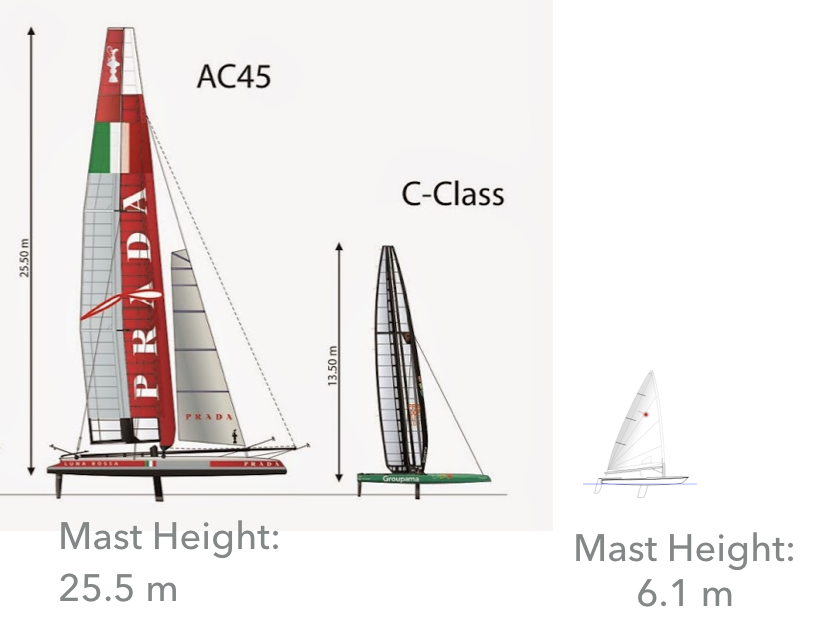
\includegraphics[width=0.75 \linewidth]{yacht_comp.png}
    \caption{Mast Height Comparison between two yachts models AC45 and C-Class versus the Laser Olympic Class, side view. \cite{yacht_compw}.}
    \label{fig:yacht_mast_height}
\end{figure}
The sailboat of the laser class is the dinghy one of the smallest boats propelled by wind, with a maximum weight of 59 kg \cite{sailoly}. Therefore its balance on the \textit{heave axis} (\acrshort{heave_ax}), between the heel angle (\acrshort{heel_ang}) and righting moment (\acrshort{right_m}) is determined by the ability of the crew to adjust its posture over each side of the boat. The posture of the crew respect to the boat is determined by the wind speed and direction mainly. So it can be said that the crew's posture is a response to the weather variations \cite{marchajaereo1979}.\par 

Even when these assumptions are implicit to keep the sailboat analyses in 2-dimensions and developed the \acrshort{vpp} there's is being some discussion about it \cite{philpott1993yacht},\cite{larsonprinciples}. The discussion are related not only with the posture but also with the impact of crew's mass (\acrshort{crew_m}). Since for Olympics Sailing Races it could represent more than $50 \% $ of the total mass of the sailboat (\acrshort{m})\cite{day2017performance}. These without considering the rate of change of these postures adjustments and the assumption that its centroid (\acrshort{crew_m}) is located in the center of gravity (\acrshort{c_g}) of the sailboat. \par 

A deeper analysis and comparison between the adaptations on the standard \acrshort{vpp} were addressed about the coefficients and forces related with the sails. The comparison of the different coefficients values include the data taken from the Offshore Rating Congress (2013) and the observations made in other works \cite{day2017performance}, \cite{carrico17symp}, \cite{binns2002development}, \cite{flay1996twisted}. Furthermore, these modifications correspond to the addition of the \textit{reef} and \textit{flat} coefficients of the sail. Particularly, they account for the fact that dinghy's sail do not reef against strong winds. As a consequence of this, the drag and lift coefficients must been adjusted during the upwind and downwind course \cite{carrico17symp}. \par \noindent
The adaptations directly related with the 
%were divided according the 
aerodynamic 
%and hydrodynamic 
forces, as a result of the \textit{flat}, \textit{twist} coefficients and the \textit{spill}(\acrshort{spill}) variable 
%were included. 
are showed next. These coefficients model the behavior of the sails and the athlete under strong wind conditions and it includes not only the upwind conditions but also the downwind course \cite{day2017performance}. % in additions to some conditions to be included when a downwind course is sailedIn \cite{day2017performance}. \par 
Therefore, equations \ref{eq:Cd} and \ref{eq:Ct} are modified to account the required adjustments. \par \noindent 
Then \acrshort{spill} modifies equation \ref{eq:Ct} and is shown in equation \ref{eq:liftMod} where \acrshort{Ctwist} has a value of  \textit{8.0} and \acrshort{twist} which is the \textit{twist variable} has a range value of [0,1], \acrshort{CDv} and \acrshort{CLmax} is obtained by interpolation from tabulated values and it depends on \acrshort{b_aw} while \acrshort{CDs} has a value of \textit{0.005} and \acrshort{ARE} is based on the rig geometry and calculated according it \cite{day2017performance}. \par \noindent  
Equation \ref{eq:Cd} is replaced by \ref{eq:draftMod}, the values taken were the smallest with an reduction of the area of 20 \% to consider shielding from the cockpit \cite{day2017performance}.\par 
%The effective aspect ratio ARE is calculated from the geometric aspect ratio based on rig geometry

\begin{equation} \label{eq:liftMod}
    C_{t}^*=C_{Dv}(\beta_{aw}-s)+C_{Dp}+f^2 \cdot C_{Lmax}^2 \cdot (\beta_{aw}-s) \cdot \Big(\frac{1+C_{twist} \cdot t^2}{\pi AR_{E}} + C_{Ds}\Big)
\end{equation}

\begin{subequations} \label{eq:draftMod}
 \begin{align}
  C_{d}^*= 1.075 && \text{for the frontal area} \label{eq:FrontalAreaDraft} \\
  C_{d}^*= 0.954 && \text{for sideways area} \label{eq:SideAreaDraft}
 \end{align}
\end{subequations}

\par 
The literature regarding \acrshort{vpp} for laser boat classes is limited and it is mainly accounted in \cite{day2017performance}, the comparisons made here are only valid for wind speed between  4 and 16 knots, while races are performed up to 25 knots. This range have to be consider in the developed of the algorithm to find the optimal path since it is the velocity of the wind that determines the direction that should be taken in order to maximize the \acrshort{vmg} criterion. \par 

\section{The Optimization Algorithm for the Minimal Time Path}
At this point, all the elements required to define the algorithm for the sailing path have been described. In this section those elements are going to be implemented in a similar order in which they were described. First the parameters of the Laser are going to be described so its \acrshort{vpp} can be estimated, then the area for the sailing race has to be defined and finally how the optimization was setting up and validated. 

\subsection{The Laser Olympic Class}
As mentioned before the Laser sailboat is the smallest class of the Olympics Sailing Classes and it is shown in figure . The dimensions and parameters that describe the laser are regulated by the \acrfull{ilca} and they are showed next in addition to some coefficients previously defined. Figure shows a side view of the Laser Standard and Laser Radial which are Olympic Classes. %For the \acrshort{Asail} and \acrshort{Asail_La} equation is used, where $L_{luff}$ refers to the luff lenght and $L_{foot}$ is the length of the foot, for which the maximum dimensions were used.
%\begin{equation} \label{eq:sail_area}
 %   A_{sail}=0.5 \cdot L_{luff} \cdot L_{foot}
%\end{equation}
\begin{description}
        \item \acrshort{mboat}= 59 [kg] \acrlong{mboat}
        \item \acrshort{Loa} = 4.2 [m] \acrlong{Loa}
        \item Beam = 1.37 [m] Beam width
        \item \acrshort{Tc} = 0.787 [m] \acrlong{Tc}
        \item \acrshort{Asail_La} = 5.76 [$m^2$] \acrlong{Asail_La}
        \item \acrshort{Asail} =  7.06 [$m^2$] \acrlong{Asail}
        \item \acrshort{Ak} = 0.23 [$m^2$] \acrlong{Ak}
        \item \acrshort{Ar} = 0.11 [$m^2$] \acrlong{Ar}
        \item \acrshort{Cdhull} = 0.02 [-] \acrlong{Cdhull}
    \end{description}
\begin{figure} [hbt!]
    \centering
    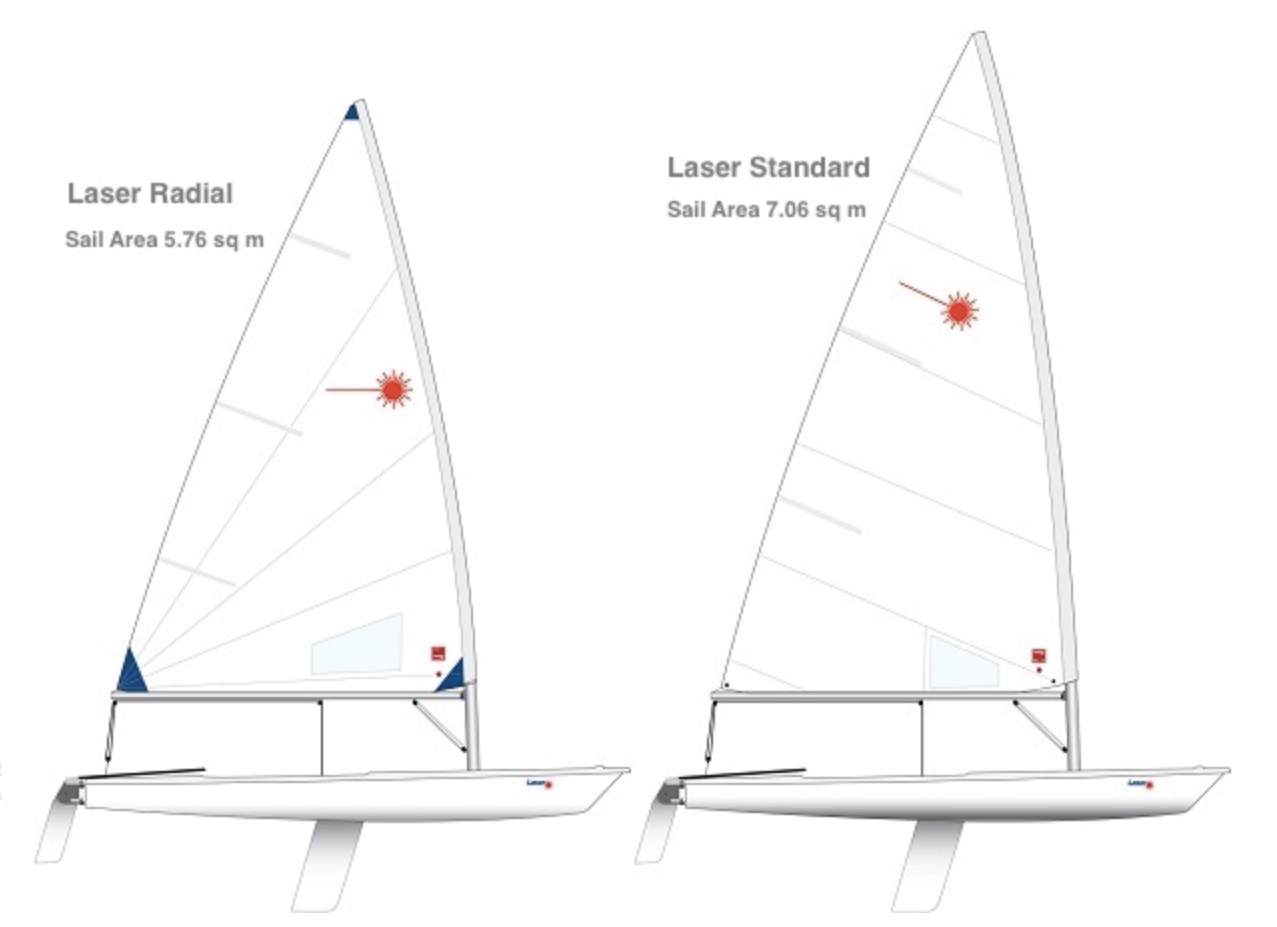
\includegraphics[width=0.64 \linewidth]{LaserOlympicClasses.png}
    \caption{Laser Olympic Classes. Laser standard refers to men category while Laser Radial is for women. The difference between them is only the size of the sail. \cite{2015LaserAssociation}}
    \label{fig:LaserSideView}
\end{figure}
The equations of section \ref{sec:eq_of_motion}, uses the added mass over each axis which according \cite{keuning2004mathematical} can be determined by equations \ref{eq:mx_add} and \ref{eq:my_add}. At this point the \acrshort{crew_m} is required and for the purposes of this research the maximum value suggested by \cite{laser_opt} is used. 
\begin{equation}\label{eq:mx_add}
    m_{x}=2\frac{T_{c}} {Loa} m_{T}=2\frac{T_{c}} {Loa} (m_{boat} + m_{c})=2\frac{0.787}{4.2}(59+70)=48.34 \text{ kg}
\end{equation}
\begin{equation} \label{eq:my_add}
    m_{y}=0.25 \cdot m_{T}=0.25 \cdot (59+70) = 32.25 \text{ kg}
\end{equation}

Most of the coefficients used on the equations of section \ref{sec:eq_of_motion} can be found on tables, however they can be approximate by using sine and cosine functions \cite{rein2012tra},\cite{moreira2011guidance}. These coefficient approximations are referred to the keel ($C_{i,keel}$) and rudder ($C_{i,rudde}$) only and they are shown next, the sub-index \textit{L} is for the \textit{lift} while \textit{D} is for the \textit{drag}. \par 
\begin{subequations} \label{eq:keel_coeff}
    \begin{align}
        C_{L,keel}=0.615sin(2\beta_{k_{a}})+0.025 \label{eq:keel_Liftcoeff}\\ 
        C_{D,keel}=-0.55cos(2\beta_{k_{a}})+0.55 \label{eq:keel_Dragcoeff}
    \end{align}
\end{subequations}
\begin{subequations} \label{eq:rudder_coeff}
    \begin{align}
        C_{L,rudder}=0.6175sin(2\beta_{r_{a}})+0.0325 \label{eq:rudder_Liftcoeff}\\ 
        C_{D,rudder}=-0.55cos(2\beta_{r_{a}})+0.55 \label{eq:rudder_Dragcoeff}
    \end{align}
\end{subequations}
Due to these approximations equations \ref{eq:Side_force}, \ref{eq:att_r} and \ref{eq:att_k} are modified and facilitate the separation of the \textit{lift} and \textit{drag} forces to use them. The angle of attack (\acrshort{a_a})is related with the \acrshort{b_aw}, therefore it is related with the trim angle of the sail (\acrshort{trim_sail}). The keel is a fix element and it is assumed rigid then its \acrshort{b_k_a} is the same as the \acrshort{b_ac}.   \par \noindent %The approximations related to the sail will not be used since equations \ref{eq:draftMod} and \ref{eq:liftMod} 
\begin{equation} \label{eq:app_current_ang}
    \beta_{ac}=atan2\frac{v}{u}
\end{equation}
\begin{equation} \label{eq:app_current_vel}
    V_{ac}=\sqrt{u^2 + v^2}=V_{boat}
\end{equation}
\begin{equation} \label{eq:keel_lift}
    F_{L,keel}=\frac{1}{2} \cdot \rho_{w} V_{ac}^2 A_{keel}C_{L,keel}(\beta_{ac})
\end{equation}
\begin{equation} \label{eq:keel_drag}
    F_{D,keel}=\frac{1}{2} \cdot \rho_{w} V_{ac}^2 A_{keel}C_{D,keel}(\beta_{ac})
\end{equation}
\begin{equation} \label{eq:angle_attack_rudder}
    \beta_{r_{a}} = \beta_{ac} - \delta_{r}
\end{equation}
\begin{equation} \label{eq:rudder_lift}
    F_{L,rudder}=\frac{1}{2} \cdot \rho_{w} V_{ac}^2 A_{rudder}C_{L,rudder}(\beta_{r_{a}})
\end{equation}
\begin{equation} \label{eq:rudder_drag}
    F_{D,rudder}=\frac{1}{2} \cdot \rho_{w} V_{ac}^2 A_{rudder}C_{D,rudder}(\beta_{r_{a}})
\end{equation}
\begin{equation} \label{eq:angle_attack_sail}
    \alpha_{a} = \beta_{aw} - \delta_{sail}
\end{equation}
The motion of the sailboat is dominated by the wind and this research is focus on the effects of the wind. As a result, the $\beta_{i_{a}}$ of the rudder and keel are treated as one component and substituted by $\alpha_{a}$ \cite{rein2012tra}. The implication of this substitution has two effects, first on the \acrshort{Rhull} and second on the lateral force. The coefficient related with the \acrshort{Rhull} has to account for thus it has to increase to \textit{0.025}. \textbf{The lateral forces is assumed to be in equilibrium all the time as a result, the \acrshort{v} velocity known as drift speed is neglected} hence equation \ref{v_dot} is omitted from the equations of motion for the Laser Class \cite{rein2012tra}.\par  
Another modification is related with equation \ref{eq:u_dot} which has to be modify to replace the hydrodynamic derivative expression ($X_{V\psi}$) by a damping expression showed on equation \label{eq:u_dotLaser}. The damping expression is related with a constant value  (\textit{Cnst}) of 0.3 according to \cite{rein2012tra}. \par
\begin{equation} \label{eq:u_dotLaserM}
    \Dot{u}=\frac{X_{TOT}}{m+m_{x}}-Cnst \cdot \Dot{\psi}^2
\end{equation}
To recapitulate all the previous changes, the equations of motion that describes the motion for the Laser Olympic Class are: \par 
\begin{equation} \label{eq:X_uM}
    X_{U}=\frac{1}{2}\rho_{w}V_{boat}^2 \cdot C_{D,hull}=\frac{1}{2}\rho_{w} \cdot V_{ac}^2 \cdot 0.025 
\end{equation}
\begin{equation}\label{eq:X_sailM}
       X_{sail}=F_{L,s}sin\beta_{aw}-F_{D,s}cos\beta_{aw} 
\end{equation}
\begin{equation}\label{eq:Forces_M} 
     X_{current}=m\cdot V_{boat} \Dot{\psi}= m\cdot V_{tc}^b \cdot \Dot{\psi}
\end{equation}
\begin{equation}\label{eq:X_TOTM}
    X_{TOT}=X_{U}+X_{sail}+X_{current}
\end{equation}
where:
\begin{equation} \label{eq:SailLiftM}
    F_{L,s}=\frac{1}{2}\rho_{a}V_{aw}^2 \cdot A_{s} C_{t}^*
\end{equation}
\begin{equation} \label{eq:SailDragM}
    F_{D,s}=\frac{1}{2}\rho_{a}V_{aw}^2 \cdot A_{s} C_{d}^*
\end{equation}
Finally the equations that describe the motion are:\par
\begin{equation}\label{eq:x_dotM}
\Dot{x}=u \cdot cos\phi + u_{tw} + u_{tc}
\end{equation}
\begin{equation}\label{eq:y_dotM}
\Dot{y}=u \cdot sin\phi + v_{tw} + v_{tc}
\end{equation}
\begin{equation} \label{eq:u_dotLaserMR}
    \Dot{u}=\frac{X_{TOT}}{m+m_{x}}- 0.3 \Dot{\psi}^2
\end{equation}

These modified equations serves only for the laser Olympic class and with them the \acrshort{vpp} can be estimated. Even so, at some wind velocities  %the approximations of 
equation \ref{eq:liftMod} %and \ref{eq:keel_coeff}
could be less accurate, specially at \acrshort{v_tw} close to 20 kn and above it. Since equations \ref{eq:liftMod} and \ref{eq:draftMod} work fine when the \acrshort{v_tw} is close to 10 kn \cite{day2017performance}, which is at the lower range of the \acrshort{v_tw} range defined by \cite{laser_opt}. \par 

\subsection{ VPP for the Laser Olympic Class}
The optimization of the minimal time path as showed in equation \ref{eq:rabaudmintime} requires to determine first the velocity which in this case \acrshort{v_aw}($\psi$). \acrshort{v_aw}($\psi$) is related with the wind speed and direction and considering the computational effort and the fact that the wind model is space and time discretized. The \acrshort{vpp} can be estimated first since the wind speed range rule ([4,25]kn) conditions the laser races. To estimate the \acrshort{vpp} not only the \acrshort{b_tw} but also the \acrshort{v_boat} has to be discretized with small steps values. \par \noindent 
Using the previous equations and replaced in equations from \ref{eq:X_tot} to \ref{y_dot} the \acrshort{vpp} can be obtained using an optimization method. The systems of equations can be solve over the angle range of [0,180 \degree] using the built-in function of \textit{fmincon} from \acrshort{matlab}\cite{rein2012tra}. The problem is defined as maximization of the \acrshort{v_boat} which means that all the forces are in equilibrium. However, any  optimization problem has to be defined in terms of the minimum value so the problem is defined as:
\begin{align}
    \text{minimize:}\qquad & -u(u,\psi,\delta_{s},V_{tw})  \label{eq:max}\\
\text{subject to:} \qquad & X_{TOT}=0 \\
 \qquad & Y_{TOT}=0
%& \Dot{v}=0 \\
%& \Dot{\psi}=0
\end{align} \label{eq:opt_vpp2}
instead of: 
\begin{align}
    \text{maximize:}\qquad & u(u,\psi,\delta_{s},V_{tw})  \label{eq:max2}\\
\text{subject to:} \qquad & \Dot{u}=0 \\
%& \Dot{v}=0 \\
& \Dot{\psi}=0
\end{align} \label{eq:opt_vpp}
Equation \ref{eq:max} shows that \acrshort{u} is the boat's velocity and it depends on itself which means that the system is not linear. Moreover, its influence on \acrshort{b_tw}, \acrshort{v_aw} determines the sail's forces. The control variables this problem are $\Dot{\psi}$ and \acrshort{trim_sail}, this last could have a value over the range of [0,180 \degree] but it should not cancel $\Psi$, during motion.
\par
\begin{figure}[hbt!]
    \centering
    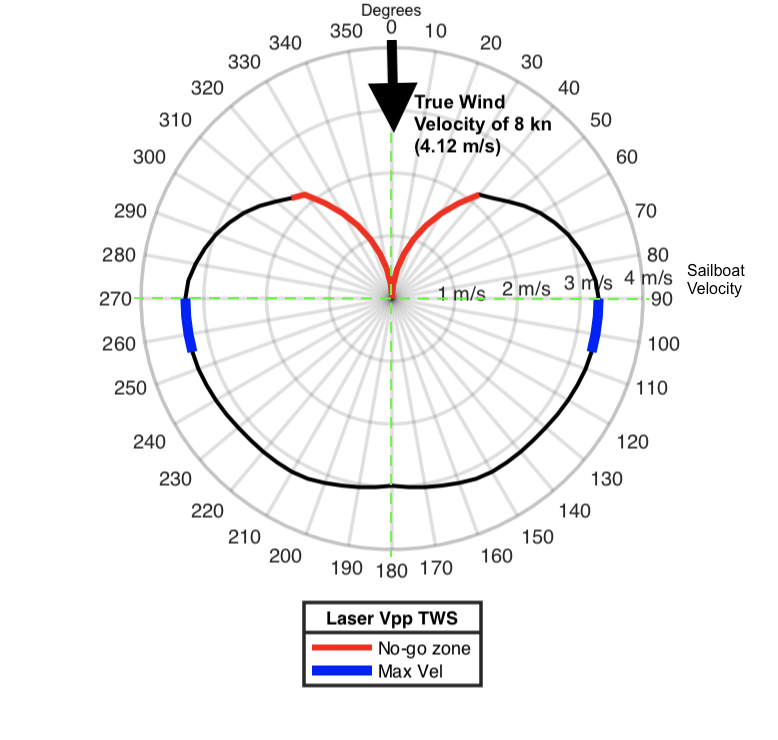
\includegraphics[width=.53 \linewidth]{Vpp_8.png}
    \caption{Full VPP for the Laser Class at 8 kn $V_{tw}$ coming at $0\degree$ from the North, the angles were discretized with and interval of $10\degree$} 
    \label{fig:Laser_Full_Vpp85}
\end{figure}
Figure \ref{fig:Laser_Full_Vpp85} shows the full \acrshort{vpp} of the Laser Olympic Class for a wind of 8 kn. In this graphic the direction of the wind is zero degrees from the North. The angle's interval is $10\degree$ and the \acrshort{v_boat} is indicated by the diameter of the circles in this case, it has a range value of [0,3.3] m$\backslash$s . In the figure the \textit{no-go-zone} is in the angle range of [0, 40] degrees and [320, 360] degrees while the maximum velocity of the boat can be reach in the angle range of [90, 115] degrees and [255, 270] degrees. \par 
\noindent
The \acrshort{v_boat} range taking out the \textit{no-go-zone} is [2,3.3] m$\backslash$s, the \acrshort{vpp} shape over the range of [90,270] degrees does no varies to much. The shape is close to a semi-circle, this means that under a downwind condition a straight trajectory could be more efficient if the tack loss time is bigger than the velocity change ratio while the \acrshort{v_tw} remains constant.  \par  

An alternative method to estimated the half of the  \acrshort{vpp} uses wind measurements for the speed and its direction. These measurements however does not have a constant interval, so to predict any other wind speed and its direction, the measured data is interpolated  
%Interpolating between known values can then give predicted maximum speeds for any true wind angle and true wind speed
\cite{philpott2001optimising},\cite{allsopp2000optimal}. For the purpose of this project, some wind measurements for wind speed  were provided by \acrlong{sailctr}. \par \noindent 
The interpolation used for the missing points was the \acrfull{pchip} from \acrshort{matlab}. The use of this data not only serves as validation for the \acrshort{vpp} calculations but also as data source. This because many of the research regarding \acrshort{vpp} for the Laser Olympic Class only cover a wind speed range of [9,12] kn \cite{day2017performance} and the measurements provided are out of this range and they are shown in figure \ref{fig:hvpp_MeasData}.\par \noindent
Figure \ref{fig:hvpp_MeasData} indicates the measurements taken with black asterisk, the rest of the points, therefore the line is the result of the \acrshort{pchip} interpolation. The wind measured are referred as \textit{TWS} and it is assumed to comes from the North, top of the graph. The \acrshort{vpp} is assumed to be symmetric and due to this, the measurements where only taken in the range of [0,180] degrees. \par 
\begin{figure} [hbt!]
    \centering
    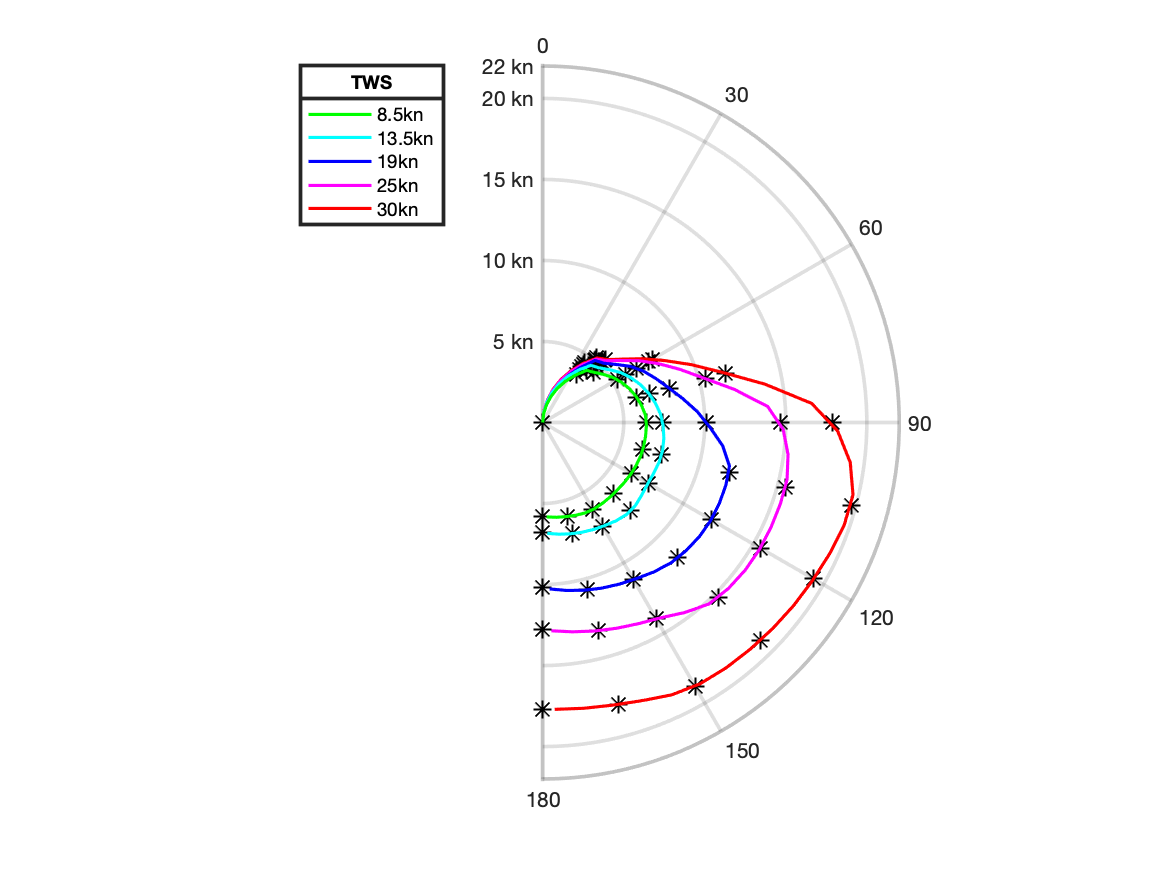
\includegraphics[width=0.72 \linewidth ]{Half_Vpp_laser2.png}
    \caption{Vpp developed with measurements provided by $InnoSportLab\textsuperscript {\textregistered}$, The Hague. The measurements are indicated with black asterisk. The results of the interpolation varies according the wind velocity (TWS)}
    \label{fig:hvpp_MeasData}
\end{figure}
The measured data not only serves to develop the \acrshort{vpp} but also to validate some of the assumptions previously made. Now that the\acrshort{vpp} was determined the formulation of the minimal time path for the Laser Sailing Class can be described.  \par 

\subsection{The Objective Function: The Minimal Time Path}
At this point all the elements required to develop the algorithm have been explained. In this section their implementation is going to take place. The objective is to find the path with the minimum time, regardless the type of sailing course. Figure \ref{fig:SailModes_Man}, shows the three types of courses with its main maneuvers and an angle range where they take place. The angle range is not specify since it depends mainly on the \acrshort{vpp} (type of sail boat) and sailor preferences. For example, under a downwind condition, many sailor prefer to follow a straight line rather than a zig-zag pattern.  \par
\begin{figure} [hbt!]
  \centering
  \subfloat[The 3 main modes to sail respect to the wind direction.]
  {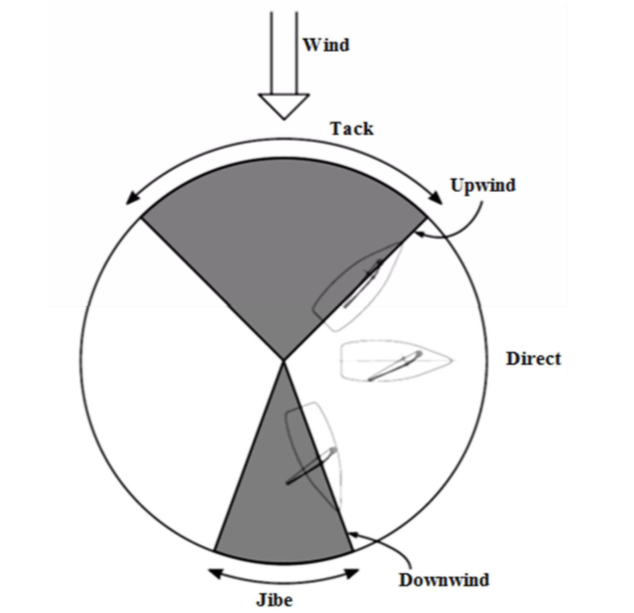
\includegraphics[width=0.45 \linewidth]
  {SailingModes.png}\label{fig:SailModes}}
  \hfill 
  \subfloat[Types of Maneuvers for sailing according the boat and wind direction .]{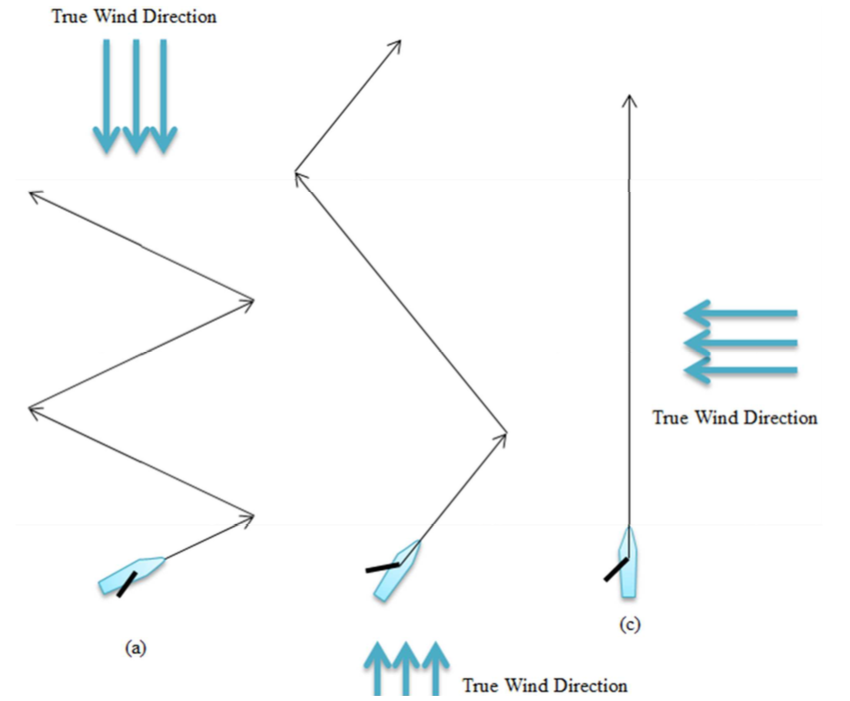
\includegraphics[width=0.5 \linewidth]
  {SailinMAnu.png} \label{fig:maneuversType}}
  \caption{Type of courses and its Maneuvers \cite{Alves2014ASailboat}}
\label{fig:SailModes_Man} 
\end{figure}

The combination of at least two of these sail-modes determines a race for Olympic Sailing Competitions. Each sail-mode over the course is defined as \textit{Leg}, them the minimal time for the race is given by the minimal time on each leg. This optimization problem is defined as a multi-phase problem, where each \textit{leg} is the phase of the problem. It is a multi-phase problem not because all the phases are connected but because on each phase different sets of constraints are implemented.\par
Each leg of the course to race is defined by the index \textit{i} and it starts at 1. %, the total number of legs on a race is 5 but this value could change.. 
The number of stages or states of the variables is defined by the index \textit{n} and it can be described as an intermediate points inside each \textit{i leg} where the time and distance are evaluated.  This means that if there are two legs in total and the number of stages is 5, therefore there are twelve stages in total (\textit{$n \times i = (5+ 1) \times 2 = 12$}).\par 
The approach of this problem is based on direction-dependence technique with the heading-angle decision to generate \textit{k} sub-routes. The reason of the \textit{k} sub-routes is to evaluate the symmetry of the \acrshort{vpp} especially at the beginning of the race.
This not only for the upwind mode and \textit{answer the question why start to port is better (or not) than start to starboard}, furthermore to evaluate the straight-line trajectory over the rest of the wind modes. \par \noindent %on the downwind and direct(reach) mode
Consequently \textit{k} is assigned to have \textit{three values}, 1 for the straight-line trajectory, 2 is for the port(left) and 3 is for the starboard (right) start direction. As a note, on the upwind condition the straight-line is not evaluated, nor optimized. Further details about \textit{k} and \textit{n} are given on coming sections of this chapter.\par 
Then the minimal time path for the Olympic Laser races is based on equation \ref{eq:rabaudmintime} and defined as follow.
The objective function is established by equation \ref{eq:minTO} and it is composed by two terms. The first term accounts for the accumulated minimal time up to the previous \textit{i leg} and it stores the  \textit{k,n} state-space variables of the previous legs, as established on equation \ref{eq:CollectPointsTime}.
The second term is the minimal time for the current \textit{i leg} from the \textit{k} sub-route over the \textit{n} stages. \par \noindent 
The time on the second term is determined by the velocity $v_{k,n}$ which depends on its heading-direction, and on the length's trajectory ($dl_{k,n}$). This means that $v_{k,n}$ is  conditioned by equations \ref{eq:C_xvel} and \ref{eq:C_yvel}, and estimated with equation \ref{eq:VelovertheLenght}.
\begin{align}
%\min_{j \in \Gamma_{i}}\\ 
    \text{min } & T=
    %\int_{t_{0}}^{t_{f}} dt=
    L_{k,n}^{i-1}(\Psi,t_{f})+ min \bigg[ \int_{t_{0}}^{t_{f}}  \frac{dl_{k,n}^i}{v_{k,n}^i} \bigg] \quad ,k \in \{1,2,3\} \label{eq:minTO}\\
\text{subject to:} \quad & \Dot{x}=u(\Psi)cos(\Psi) + u_{tw}+u_{tc} \label{eq:C_xvel} \\
\quad & \Dot{y}=u(\Psi)sin(\Psi) + v_{tw}+v_{tc} \label{eq:C_yvel}
\end{align}
where:
\begin{equation}\label{eq:CollectPointsTime}
     L_{k,n}^{*}(\Psi,t_{f})=[x_{k,n}, y_{k,n},t_{f}]^{*}
\end{equation}
\begin{equation}\label{eq:VelovertheLenght}
     v_{k,n}^{*}=\sqrt{\Dot{x}^2+\Dot{y}^2}
\end{equation}
The boundary conditions showed on equations \ref{eq:locIniX}, \ref{eq:locFinX}, \ref{eq:locIniY} and \ref{eq:locFinY} are determined by the leg, particularly by the location of the start buoy and end buoy. These buoys are located over the sailing area and they determine the direction of the boat to follow along with the direction of the wind, to arrive to the next buoy. The location of each buoy is provided in Cartesian coordinates, as explained in \ref{sec:RefFrames}, the latitude-longitude coordinates can be converted to [X,Y] using the \acrshort{matlab} function \textit{deg2utm(Lat,Lon)}. Equation \ref{eq:InitialTime} defines the initial time for the first leg (\textit{i=1}) which is zero. The initial time for the next leg is given by the final time of the previous leg, as shown in equation \ref{eq:FinalTimeLeg}.
\begin{align}
    \quad & x_{k}(0)^i=x_{1}\label{eq:locIniX} \\
    \quad & x_{k}(t_{f})^i=x_{2}\label{eq:locFinX} \\
    \quad & y_{k}(0)^i=y_{1}\label{eq:locIniY} \\
    \quad & y_{k}(t_{f})^i=y_{2}\label{eq:locFinY}\\
    \quad & t_{0}^1=0 \label{eq:InitialTime} \\
    \quad & t_{0}^{i}= t_{f}^{i-1} \label{eq:FinalTimeLeg}
\end{align}
To connect all the legs, and predict the optimal time path for the whole race, the next equations \ref{eq:x_linkC} and \ref{eq:y_linkC}, gives continuity to the path. This continuity helps the algorithm to control the tack maneuver and estimate the tack angle for each leg change.
\begin{align}
    \quad & x^{i+1}(t_{0}^{i+1})=x^{i}(t_{f}^{i})\label{eq:x_linkC}\\
    \quad & y^{i+1}(t_{0}^{i+1})=y^{i}(t_{f}^{i}) \label{eq:y_linkC}
\end{align}
The tack maneuver refers to the change in direction due to a change of a leg, in other words it is a transition maneuver. This transition maneuver or the turn/tack angle is the angle between the end section (stage) of one leg with the start  section (stage) of the next leg and it is constrained by two equations showed as follow and in figure \ref{fig:tackAngL}.\par
\noindent
for the tack to port:
\begin{equation}\label{eq:tackportC}
40\degree < \Psi_{n_{max}-1}^{i}(t_{f}^{i}) -
\Psi_{n+1}^{(i+1)}(t_{0}^{i}) < 130 \degree
\end{equation}
\noindent
and for the tack to starboard:
\begin{equation}\label{eq:tackstarbC}
-130\degree < \Psi_{n_{max}-1}^{i}(t_{f}^{i}) -
\Psi_{n+1}^{(i+1)}(t_{0}^{i}) < -40 \degree
\end{equation}
\begin{figure} [hbt!]
    \centering
    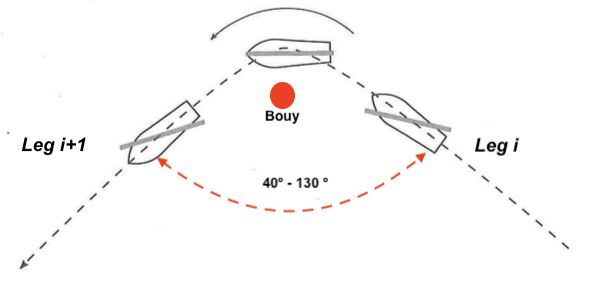
\includegraphics [width=0.55 \linewidth]{tack.png}
    \caption{Tack angle range between legs.}
    \label{fig:tackAngL}
\end{figure}
The final time on each leg is the minimal time and the result of the optimization over that \textit{i leg} and \textit{k} start direction. However, it is known that on the upwind condition, the Laser follows a zig-zag pattern to move against the wind. Moreover, each of these changes in direction takes time and speed and this have to be quantify. For example, \cite{rein2012tra} mentioned a speed loss of 2 kn due to change in direction, other authors refers to these changes as a delay in time of about 5 to 10 seconds before they are reflected in the trajectory \hl{(\textbf{find reference from ch1 and ch2})}. \par \noindent
In this algorithm the number of changes in the trajectory is quantify as a time loss added to the final time on each leg by equation \ref{eq:FinalTime}. The time loss to add of equation \ref{eq:Tot_TimeLoss} depends on the total number of changes in direction during the \textit{i leg}, set on equation \ref{eq:shiftDirCount}, multiple by a constant defined as a $t_{tack-loss}$ and its value is defined in further sections on this chapter. In addition, equation \ref{eq:shift_Dir} controls these shifts in direction so changes larger than 180 \degree  does not happen.
\begin{equation}\label{eq:shift_Dir}
    0 \degree <=\Psi_{k,n+1}^{i}(t_{f}^{i}) - \Psi_{k,n}^{i}(t_{0}^{i}) <180 \degree
\end{equation}
\begin{equation} \label{eq:FinalTime}
    t_{f}^{i}=t_{f}^{*i} + \Delta T_{loss}^i
\end{equation}
\begin{equation} \label{eq:Tot_TimeLoss}
    \Delta T_{loss}^i=t_{tack-loss} \sum_{n=1}^{n} \Delta \Psi_{k}^* (i)
\end{equation}
\begin{equation} \label{eq:shiftDirCount}
\Delta\Psi_{k}^*(i)=
\begin{cases}
0, \quad  \text{if: } \Psi_{k,n+1}^{i}(t_{f}^{i}) = \Psi_{k,n}^{i}(t_{0}^{i})\\
\\
1 %\quad  \text{if: } \Psi_{k,n+1}^{i}(t_{f}^{i}) \neq  \Psi_{k,n}^{i}(t_{0}^{i})\\
\end{cases}
\end{equation}
\begin{equation} \label{eq:TimeFinal_acum}
    t_{f}^{*i}=\sum_{i=1,k}^{i} \Big( t_{f}^{i,k} - t_{0}^{i,k} \Big)
\end{equation}
The state-space limits for the variables are defined in equation \ref{eq:xlox_leg_alt}, \ref{eq:ylox_leg_alt} and \ref{eq:Dirlox_leg_alt}.  The first two limits the position of the sailboat while the last limits the heading angle ($\Psi$) to evades the \textit{no-go-zone}.
\begin{align}
    \quad & x_{min}^{i,1}<x(t)_{n}^{i,1}<x_{max}^{i,1} \label{eq:xlox_leg_alt}\\
   \quad & y_{min}^{i,1}<y(t)_{n}^{i,1}<y_{max}^{i,1} \label{eq:ylox_leg_alt}\\
   \quad & \Psi_{min} <\Psi(t)< \Psi_{max} \label{eq:Dirlox_leg_alt} \\
  \text{where:} \quad & 40\degree  <\Psi(t)< 320\degree \nonumber 
\end{align}
 As mentioned before on each leg the state-space constraints are different, to determined these limits the coordinates of the mid-point of the straight-line trajectory (\textit{k=1}) between buoys is required. The tolerance factor $x_{SAtot}$ and $y_{SAtot}$ determine the minimum and maximum values of the coordinates and defined the limits on each leg. The next equation shows how these estimations are done. In the case of the minimum value or lower bound, it requires the minimum coordinate for \textit{X} and \textit{Y} coordinates from the \textit{3 sub-routes} while for the upper limit it is the maximum of them, in both cases it is also required the $x_{mean}^{i}$ \textit{mean values from the 3 sub-routes (k) }. \par 
 
 The value of this factor should be chosen carefully, one of the reason is that a bigger area not always have more nodes, and the algorithm will take more time to estimate the optimal solution. Moreover it is possible that a local minimum will be find instead of the global solution, because of this it was suggested to run the algorithm several times  guessing some of the initial conditions. The next iterations serves to tune this conditions until they remain the same \cite{philpott1993yacht}. %and changing them for the next time. If the solution remains the same the solution is the optimal, otherwise  
\begin{equation} \label{eq:Xmin_SailArea}
    x_{min}^{i}=x_{mean}^{i} - x_{SAtol}\cdot \Bigg[ x_{mean}^{i} -  min \bigg( x(t_{0}^{i})^{i},x(t_{f}^{i})^{i} \bigg) \Bigg]
\end{equation}
\begin{equation} \label{eq:Xmax_SailArea}
    x_{max}^{i}=x_{mean}^{i} + x_{SAtol}\cdot \Bigg[ x_{mean}^{i} -  max \bigg( x(t_{0}^{i})^{i},x(t_{f}^{i})^{i} \bigg) \Bigg]
\end{equation}
\begin{equation} \label{eq:Ymin_SailArea}
    y_{min}^{i}=y_{mean}^{i} - y_{SAtol}\cdot \Bigg[ y_{mean}^{i} -  min \bigg( y(t_{0}^{i})^{i},y(t_{f}^{i})^{i} \bigg) \Bigg]
\end{equation}
\begin{equation} \label{eq:Ymax_SailArea}
    y_{max}^{i} = y_{mean}^{i} + y_{SAtol}\cdot \Bigg[ y_{mean}^{i} -  max \bigg( y(t_{0}^{i})^{i},y(t_{f}^{i})^{i} \bigg) \Bigg]
\end{equation}

The optimization problem and its constraints for the minimal time path for the Laser Class has been defined. These constraints not only helps the algorithm to get the optimal solution but also to connect all the legs. The connection between legs is made by means of the tack angle, a simplify approach followed for the purposes of this research \cite{jouffroy2009steering}, \cite{LinXiao2011ModelingYachts}.\par 
The state-space constraints are coupled not only withe the wind forecast model but with the course of the competition. Even when some space boundaries varies according to the leg to course, it is the orientation of leg relative to the wind angle the parameter that tune the boundaries of this area. For this reason, a further section will explain how the integration of the curse is made, more precisely the locations of the buoys into the minimal time path trajectory.\par 

% which is simplification approach to acknowledge.    For more details review 
 \subsection{Definition of the Sub-routes (\textit{k=2,3}) at port and starboard direction}

The optimization algorithm initialize with 3 alternative sub-routes and they are defined by the \textit{k} index, moreover, these sub-routes are defined in the same way for any leg. The reason of them is not only because of the heading-angle approach but also because the \textit{fmincon} function from \acrshort{matlab} request initial values of the variables used on the cost function to find the optimal solution of the problem by starting at different points \cite{mitchell2000geometric}, \cite{kelly2015transcription}. \par 

Starting at different points allows the conversion of the solution, however in this case it also aim to the strategy of the race for coaches and athletes. In addition, it aims to limit the area within the optimal path is found and reduces the computational effort also. Because the \acrshort{vpp} has a non-convex shape a path attainable region can be define, the implication of a non-convex \acrshort{vpp} implies that the optimal path may not be unique \cite{dolinskaya2012time},\cite{dolinskaya2013fastest}.  For example, on the upwind condition the maximum velocity is found after the 40\degree, and there are two possible trajectories to follow and reach the next buoy using also the \acrshort{vmg} criterion. \par 
First, at 45\degree the sinus and cosine functions have the same value and it is out of the \textit{no-go-zone}. This means that it possible to sailing at 45\degree respect to the wind direction until the mid-point %on the \textit{X-coordinate} 
and then tack at -45\degree until the target buoy is reached. By doing these tacking maneuvers on both directions port and starboard directions, the sailing area for each leg can be setup. This area can also can be stretching using the $x_{SAtol}$ and $y_{SAtol}$, this is done to give additional space for possible wind shifts, \cite{xing2012path}. \par \noindent
The second alternative is to tack at 45\degree until the target buoy can be reach by making a turn of 90\degree respect to the wind. This alternative was not followed, first because even when the velocity at 90 \degree is the fastest the distance to sail is the larger. Moreover under a constant wind speed and  direction, the ratio between the distance to sail versus the ration between velocities is larger. Therefore, there is no advantage to sail at a higher velocity because the distance to cover does no compensate the increment on the velocity and this only increase the time to reach the target buoy. \par 
\begin{figure}[hbt!]
    \centering
    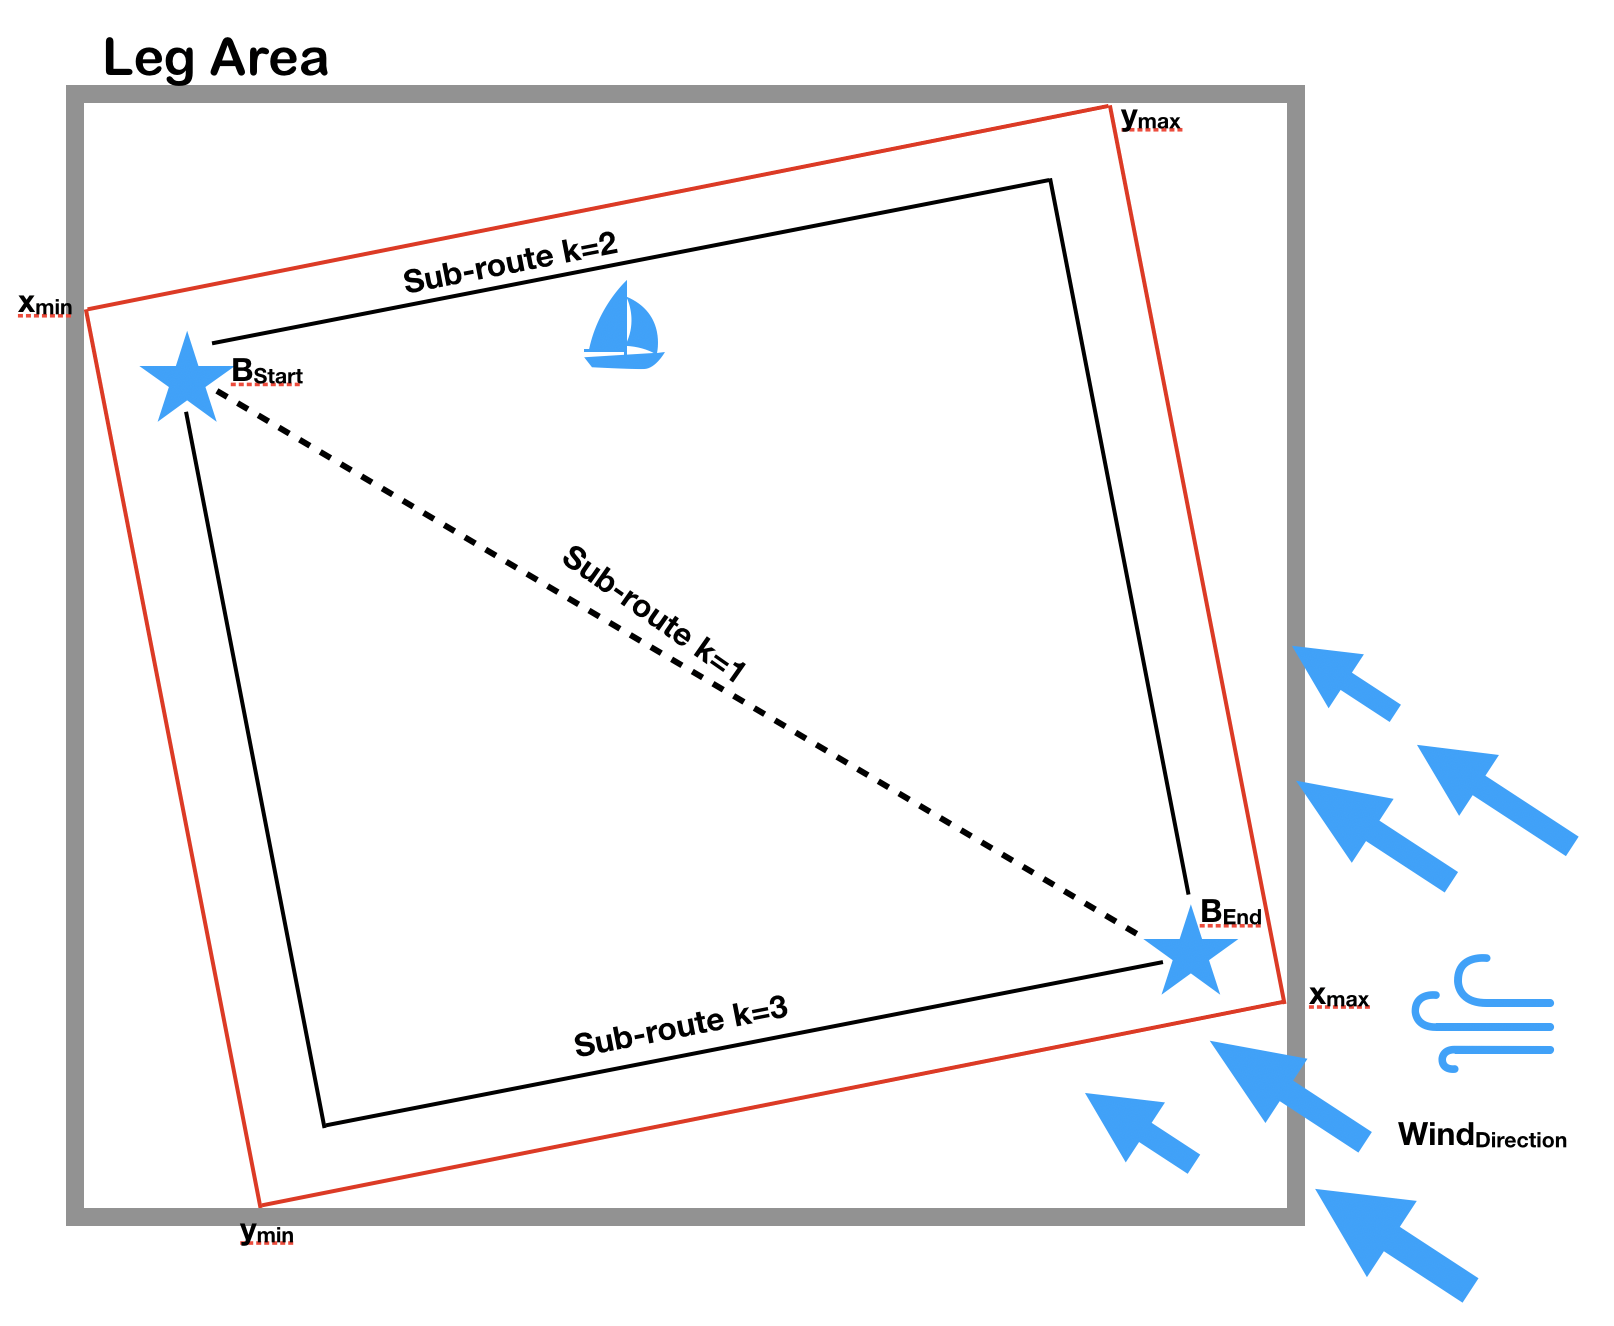
\includegraphics[width=0.5 \linewidth]{LegSail.png}
    \caption{Example of a Sail Area for a Leg using the sub-routes}
    \label{fig:LegSailArea}
\end{figure}
Following the first alternative 2 sub-routes where developed one for the port direction which is assigned by \textit{k=2} and the other to starboard assigned by \textit{k=3}. For the rest of the wind conditions the same approach is followed to define these two sub-routes and therefore the bounds for the sailing area on each leg.  \par
The \textit{n} stages of each sub-route are located within each sub-route so \textit{n} are points defined by \textit{[X,Y]} coordinates and its location determines the path to followed for a particular leg. In addition to this \textit{n} stages, a number of intervals between them were defined to describe properly the $dl_{k,n}^{i}$ of the objective function (equation \ref{eq:minTO}).  This number of intervals and the \textit{n} stages are designated at the beginning of the algorithm and they are part of the initialization parameters a large number for the interval value is recommend to have a smooth path, so the interval is designed by equation \ref{eq:interval}. For example, \textit{9 stages} with \textit{100 intervals} it generates \textit{1010} length elements per sub-route. 
\begin{equation} \label{eq:interval}
   \text{Interval: }  m=100
\end{equation}
\begin{equation} \label{eq:interval-example}
  elements_{dl}=(n+1) \cdot (m+1)
\end{equation}
These sub-routes serves to defined the limits on each leg, not by the means of coordinates of each point but by the maximum and minimum value of those coordinates. The shape of the area for each leg is a rectangle where the coordinates of the opposite corners are defined as equations \ref{eq:Xmin_SailArea}, \ref{eq:Xmax_SailArea}, \ref{eq:Ymin_SailArea} and \ref{eq:Ymax_SailArea} and example of this area is showed in figure \ref{fig:LegSailArea}.\par 
%Because inside each leg numer of \textit{n} st
%The algorithm is build in states (\textit{n}) inside each leg \textit{n}) , along each stage the dl will take place. The reason of this is to control the number of tacks along the leg, and in such way the zig-zag could be define.
\subsection{Course Integration into the Time Optimization Path Algorithm} \label{sec:Coure_LegIntegration}

The setup of the course is defined by the organizers of the event and this is done with the a diagram and with the location of the buoys using \textit{latitud-longitud coordinates}. The importance of them is because the space constraints explained before are linked with the legs of the course which in consequence are related with the buoy's location. The location of the buoys define the distance to sail, the angle direction of the leg respect to the wind direction and as result the wind mode to sail. \par 

An example of the information about the course is showed in figure \ref{fig:Rio_Course1} and it shows a \textit{trapezoid course}, where the start and end of the competitions is defined by a line. In this course there are 6 buoys, 2 line indicator and 2 boats. The letter next to the number of the buoy indicates it locations respect to the boat, so \textit{s} is for \textit{starboard} and \textit{p} for \textit{port}. The order of the marks, indicated in the table below of the diagram, describes how the legs are designated and the code or signal for that sequence. The coordinates of the buoys are provided previous to the race, since they depend on the wind direction and other factors.  \par 
\begin{figure} [hbt!]
    \centering
    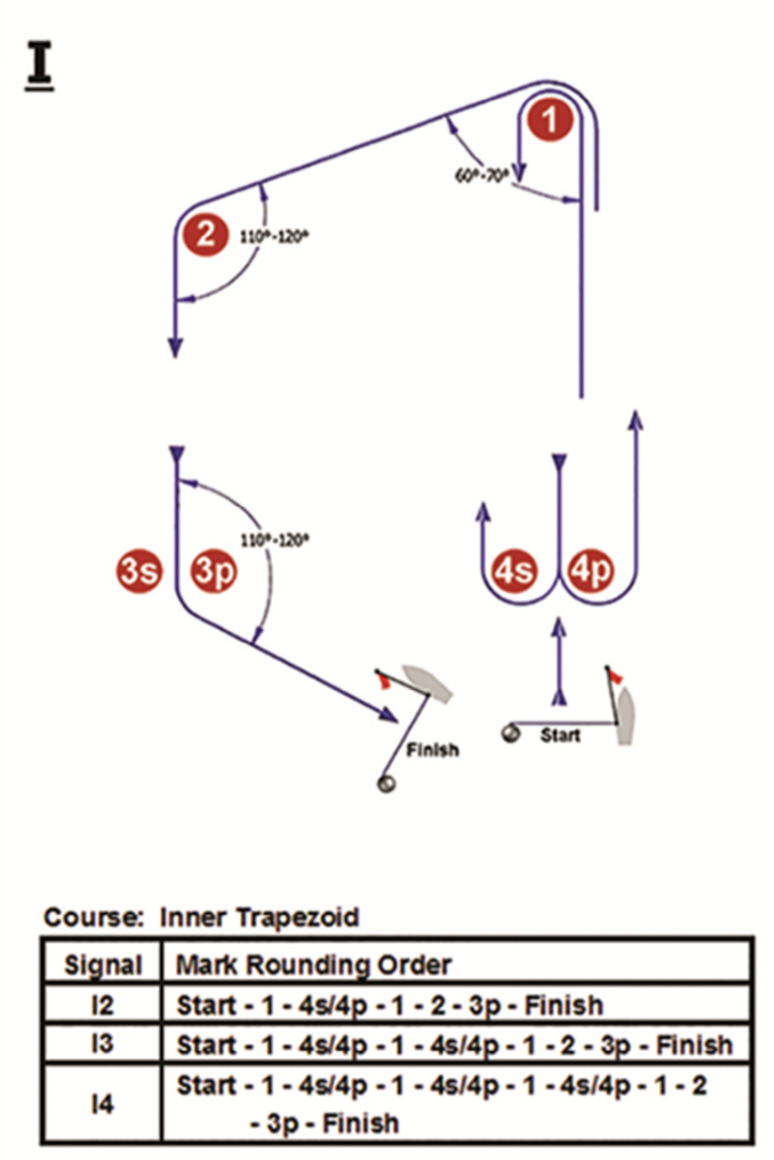
\includegraphics[width=0.39 \linewidth]{course_rio.png}
    \caption{The I Trapezoid Course diagram provided for the Sailing competitions on Rio 2016 Olympics \cite{sailoly}.}
    \label{fig:Rio_Course1}
\end{figure}
For the purposes of this research, the marks where a line is defined or where 2 buoys are designated with the same number, a mid point is going to be calculated to represent this condition. However, for the start and the end line the location of both ends is considered and the mid point is also going to be calculated. The reason of these three points, on the start and on the end line is to account the variation of the wind direction and review how sensible is the time path on the first leg and on the last leg. \par

The location of the buoys most of the time is provided in \textit{latitud-longitud coordinates} and the units are degrees-minutes-seconds, before to convert them to \textit{[X,Y] coordinates} they need to be converted to degrees. This conversion is made using the \textit{dms2degrees} from \acrshort{matlab}. Once this conversion is done, and using the order of the buoys the algorithm will estimate the distance between them with the \acrshort{matlab} function \textit{pdist($b_{1},b_{2}$,'euclidean')}. \par \noindent The angle between them is based on the normal plane, since the wind angle is respect to the \textit{Norht} it is determined in degrees by equation \ref{eq:bouy_angle}, where \textit{i} is the index related to the leg. However, even when this expression only refers to the leg, it can be used to estimate the heading-angle($\Psi$) and  therefore $dl_{k,n}^{i}$. \par 

\begin{equation} \label{eq:bouy_angle}
    \theta_{{i}}=atan2d \bigg [\frac{x_{2}-x_{1}}{y_{2}-y_{1}} \bigg] ^{i}
\end{equation}

The wind mode of the leg is given by the difference between %the angle of the leg 
\acrshort{ang_bouy} %respect to the wind and
and the wind angle, %for now on it is defined as \textit{\acrshort{twd}} instead of 
\acrshort{b_tw}, depending on the difference between those angles the wind mode and its angle are defined by equation \ref{eq:wind_modesDef}. The wind mode angle of the leg (\acrshort{angLegWind}) is defined at the beginning of the competition (\textit{$t_{0}$}), in order to start the calculations of the sub-routes. In this case, %The \acrshort{twd} 
the \acrshort{b_tw} only depends on time in the next section is going to be explained how this value is determined since in section \ref{sec:SailinArea_WindModel} it was explained that it depends on 4 dimensions.\par 
\begin{equation} \label{eq:wind_modesDef}
\Omega_{i,t_{0}} = \mid \theta_{i}-\textrm{TWD}_{t} \mid,
- \quad 
    \begin{cases}
        \text{Upwind(Upw)} \quad &
            \begin{cases}
                0\degree  &\leq  \mid \theta_{i}-\textrm{TWD}_{t} \mid    \leq    45\degree \\
                315\degree  &\leq    \mid \theta_{i}-\textrm{TWD}_{t} \mid  \leq   360\degree \\
            \end{cases} \\ 
    \\
        \text{Direct(Rch)}\quad &
            \begin{cases}
                45\degree   &<     \mid \theta_{i}-\textrm{TWD}_{t} \mid \leq   135\degree \\
                225\degree &\leq \mid \theta_{i}-\textrm{TWD}_{t} \mid <  315\degree \\
            \end{cases}\\
    \\
        \text{Downwind(Dwn)}\quad &
            \begin{cases}
                135\degree &<  \mid \theta_{i}-\textrm{TWD}_{t} \mid <  225\degree \\
            \end{cases}
            
    \end{cases}\\
\end{equation}
The buoys and its orientations respect to the wind define the legs and the limits of the area for each leg using the sub-routes as a reference. The \acrfull{angLegWind} determines the maximum velocity that the sailboat can achieve, once the intensity and location of the boat is known.  Now that the parameters for the course on each leg are defined, the next section will explained how the wind model is going to be integrated into the algorithm. \par 

\subsection{Coupling the Wind Model with the Sail Course} \label{sec:SailinArea_WindModel} %for the Time Optimization Path Algorithm
Until now, the optimization algorithm has been described along with the state-space constraints only in terms of space coordinates. In the other hand, section \ref{sec:WRF_WindM} has described the \acrshort{wrf} wind model in general, while section \ref{sec:WRF_WindM_FR} provide all the details for the model used on this research. To move the sailboat not only it needs a target but also to know the wind velocity \acrshort{v_tw} at a specific time and location.\par \noindent %where is going to be head sailboat from one point to another it the
This section describes how the wind model of section \ref{sec:WRF_WindM_FR} is integrated into this algorithm, so equation \ref{eq:VelovertheLenght} can be determined. The reasons of this integration and adaptation, first, is because the area covered by the \acrshort{wrf} wind model of section \ref{sec:WRF_WindM_FR} is much larger than the area of the course. Second, the time step ($\Delta t$) is about 10 minutes, meaning that the wind characteristics remain constant along this $\Delta t$. However, it is most probably that the space-time dimensions for the estimation of the \acrshort{v_tw} does not corresponds exactly with the space-time coordinates of the grid from the \acrshort{wrf} model despite this its value has to be estimated. \par \noindent Moreover, the time at which the competition starts has to be included during the initialization of the algorithm in addition to the duration of the race and some delays, all this factors are considered for the definition of the \textit{time window}.\par

Previous to the race date, the location of the sail course and the estimated time to start it are known. If the conditions are not meet the race could be delay until this they are meet or in the worst case scenario, the race could be canceled. Because of this, using the start time and the duration of the race (estimated to be about \textit{one hour}). The \textit{time window} is estimated by equations \ref{eq:time_window0} and \ref{eq:time_windowf} adding a bonus time or tolerance up to \textit{three hours} for the upper limit and subtracting \textit{two hours} for the lower limit.

\begin{align} %
    \textrm{Time window} &=\big[\textrm{Time window}_{0},  \textrm{Time window}_{f} \big]\label{eq:time_window}\\
    \textrm{Time window}_{0}&=\textrm{Time start}_{floor}-\textrm{Lower Tolerance} \label{eq:time_window0}\\
    \textrm{Time window}_{f}&=\textrm{Time start}_{ceil}+\textrm{Upper Tolerance}+\textrm{Duration}_{Race} \label{eq:time_windowf}
\end{align}

The tolerances are not the same for both limits because due to the weather conditions most of the time the competition could be delay rather than changed for and earlier time. In cases where the time is not defined in hours only, the start time is rounded to a \textit{floor} value, while for the end time it is rounded to a \textit{ceil} value. The round or floor value in this case is setup for an integer hour value, but it can be change for half-hour or any other value. For example, if the start time is 13:25 hrs, the time window is:
\begin{align} %\label{eq:time_window}
   \begin{split}
        \textrm{Time window}_{0}&= 13:25\textrm{ hr}_{floor} -\textrm{2 hr}\\ 
        &= 13:00\textrm{ hr} - 2\textrm{ hr}
   \end{split} \label{eq:time_window0Ex}\\
    \begin{split}
        \textrm{Time window}_{f}&=13:25\textrm{ hr}_{ceil}+\textrm{3 hr}+\textrm{1 hr}\\
        &= 14:00 \textrm{ hr} + 3\textrm{ hr} +1 \textrm{ hr} \label{eq:time_windowfEx}
    \end{split}
    \\
    \textrm{Time window} &= \big[11:00,18:00 \big]
\end{align}

The definition of the \textit{time window} helps to reduce the length of the \textit{time dimension} from the \acrshort{wrf} wind model. For example, on section  \ref{sec:WRF_WindM_FR} it was mentioned the size of their dimensions, which are (\textit{x,y,z,t}) 198 $\times$ 301 $\times$ 50 $\times$ 145, since $\Delta t = 10$ minutes. Using the previous example of the \textit{time window}, this means that instead of using the 145 time-datasets only \textit{43} time-datasets are used on this algorithm. This reduces the time of processing for this model since only aprox. $30\%$ of them are used to determine the solution of the minimal time path.\par 

Previous to the competitions, with a couple of months in advance, the location and diameter of the course area is communicated to the participants. Using these information, without any details about the location of the buoys, the area from the wind model for this algorithm is defined as a circle inscribed in a square. The coordinates of the opposite corners of this square are modified as equations \ref{eq:Xmin_WindArea},\ref{eq:Xmax_WindArea},\ref{eq:Ymin_WindArea} and \ref{eq:Ymax_WindArea} indicate. The tolerance of the wind area is determined by the radius of the sail course multiplied by \textit{n} times the grid space  ($\Delta x$) of the \acrshort{wrf} wind model. \par
\begin{equation} \label{eq:Xmin_WindArea}
    X_{W,min}= X_{CTR,course}-\frac{\clock_{course}}{2} \cdot n \Delta x
\end{equation}
\begin{equation} \label{eq:Xmax_WindArea}
    X_{W,max}= X_{CTR,course} + \frac{\clock_{course}}{2} \cdot n \Delta x
\end{equation}
\begin{equation} \label{eq:Ymin_WindArea}
    Y_{W,min}= Y_{CTR,course}-\frac{\clock_{course}}{2} \cdot n \Delta x
\end{equation}
\begin{equation} \label{eq:Ymax_WindArea}
    Y_{W,max}= Y_{CTR,course} + \frac{\clock_{course}}{2} \cdot  n \Delta x
\end{equation}

The value of \textit{n} depends on the size of the grid, $\Delta x $, respect to the \textit{radius} of the course as indicated in equation \ref{eq:n_windTolerance}. Since the  \cite{race_pol2017} establishes that the trapezoid course must be contained in this area, so \textit{n} is the next integer value from the ratio between them. If the coordinates of the buoys are known, the minimum and maximum value of all of them are used instead of the coordinates of the center of the sail area to define the corners of the wind area. \par % and the limits for the wind model are defined in a similar way. \par 
%\begin{equation}\label{eq:WRF_windArea}
%\end{equation}
\begin{equation} \label{eq:n_windTolerance}
    n=\lceil \frac{\clock_{course}}{2 \cdot \Delta x}
\end{equation}
%\begin{equation} \label{eq:TolWindArea}
%2\cdot \Delta x =
%\begin{cases}
%\Delta x \textrm{,} \quad & \Delta x < 1000\\
%\Delta x\textrm{,} \quad & \Delta x 
%\end{cases}
%\end{equation}

Using the previous equation the wind area is defined for this algorithm and it is larger than the area of the course, figure \ref{fig:WindAreaSketch} sketch this concept. It shows that if the center of the sail area is sufficiently far for any grid data-point, for example, within a sail of area with a $\clock = 3 \Delta x$ it only contains \textit{four} data-points while within the wind area defined with the previous equations it contains 64 data-points.\par

It is important that regardless the location or time, the algorithm should be capable to estimate the wind's velocity. % at any time and location. 
Particularly when the coordinates are not coincident with those of the grid from the wind model. Thus to estimate the velocity at any point over the space and time an interpolation method is required. The data-points around the point of interest must be enough to estimate this value, moreover the area defined for the wind.  \par 
%For example, %if the location is close to the limits of the sail area, the available datapoints are sufficient and the interpolation can be made without compromising 

\begin{figure} [hbt!]
    \centering
    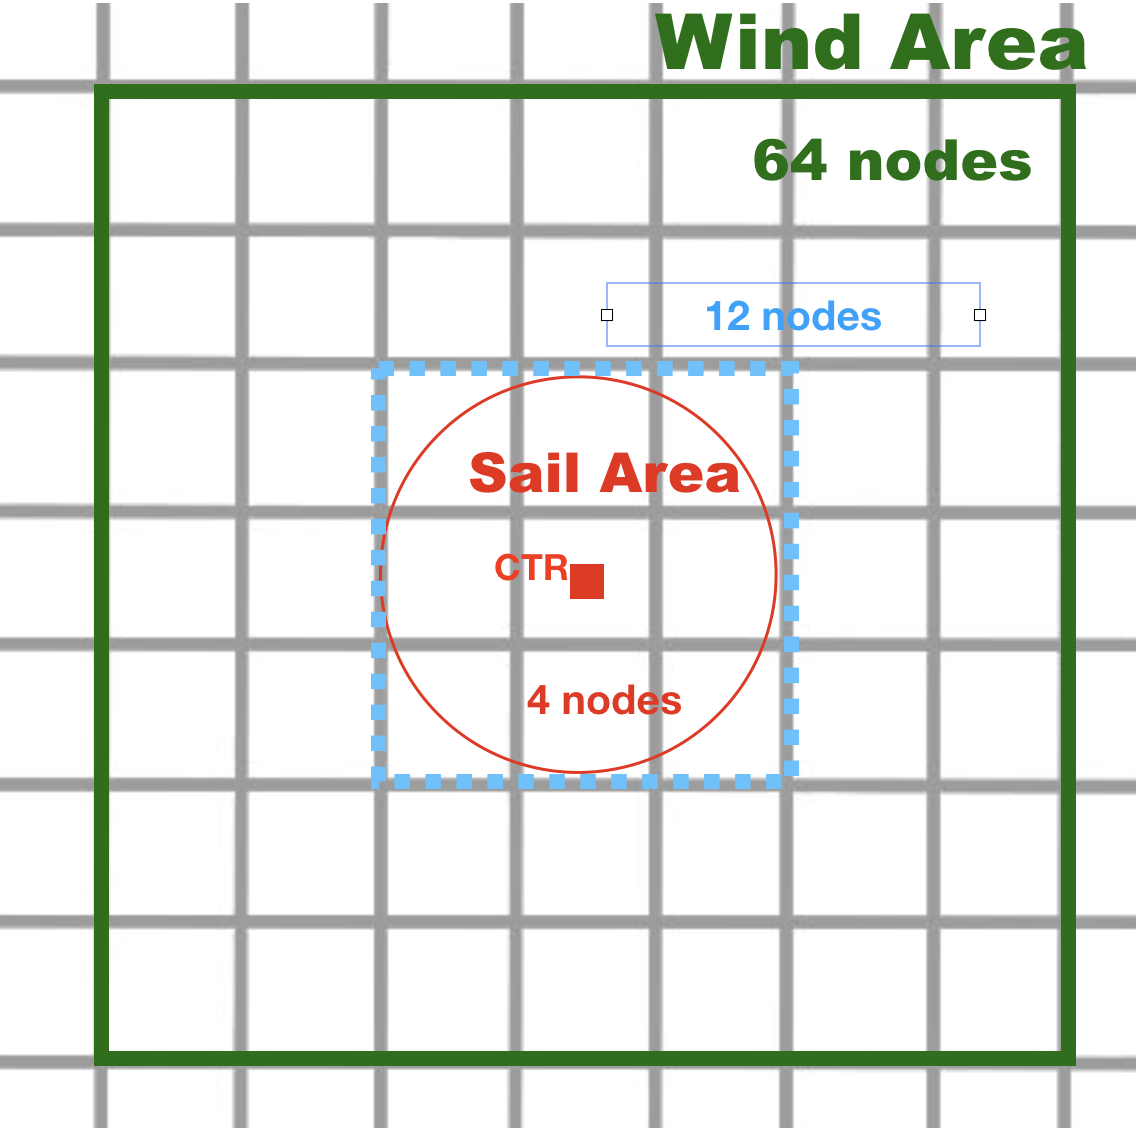
\includegraphics[width=0.32 \linewidth ]{gridWind.png}
    \caption{Wind Area Concept using a wind model representation. The inscribed sail area shows the limits of the square and its corners are used for the definition of the wind area.}
    \label{fig:WindAreaSketch}
\end{figure}

The interpolation method used in this algorithm is the \textit{griddata} function from \acrshort{matlab}. This function-method estimate the components of the wind's velocity %($u_{tw}$ and $v_{tw}$) at any time and position 
using the coordinates from the grid arrangement of the \acrshort{wrf} wind model. Figure \ref{fig:gridDataInterpo} shows a graphical representation of how this function and the wind model interacts. It shows how two datasets for the velocity with coordinates \textit{[X,Y,t]} are used to determine the velocity $V_{tw}^{*}$ at $t^{*}$ which is intermediate from $t_{0}$ and $t_{1}$. Inside the function to obtain the requested value, a method has to be defined in cases where a liner interpolation doesn't apply. %for the interpolation of the values 
For the velocities, in this research, the \textit{nearest} option for the method is used inside the \textit{griddata} function.\par

\begin{figure}[hbt!]
    \centering
    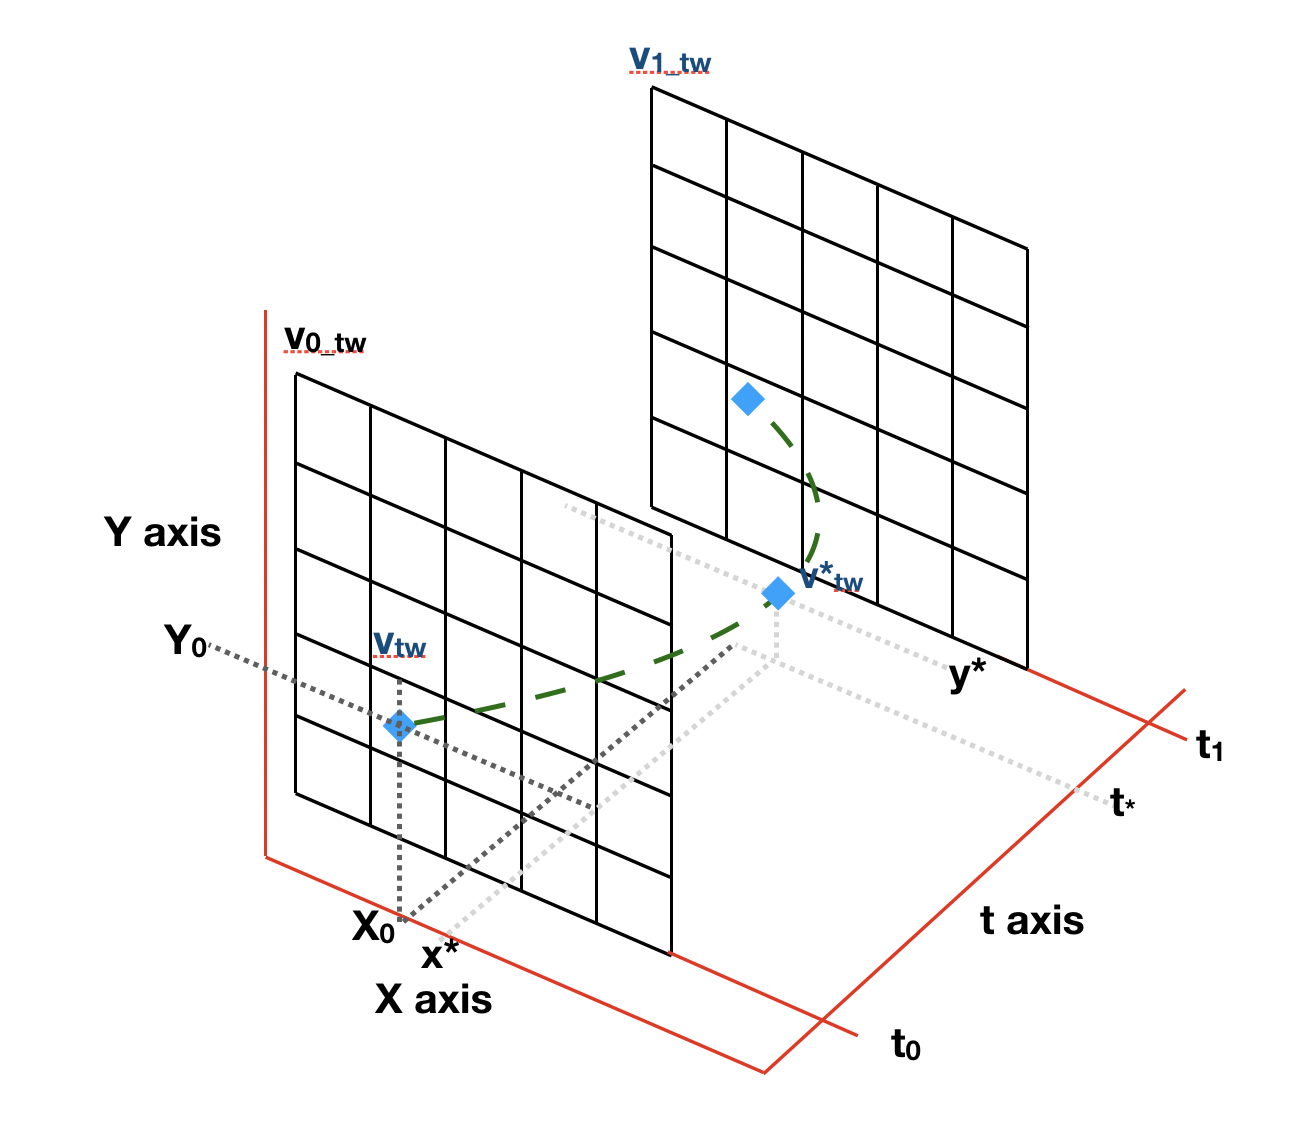
\includegraphics[width=0.45 \linewidth]{gridDataInterp.png}
    \caption{Griddata Method, graphical representation of two datasets. The function interpolates the coordinates and values from the grid to obtain any intermediate value}
    \label{fig:gridDataInterpo}
\end{figure}

The coordinates used along this algorithm are \textit{[X,Y,t]}, this means that any data using \textit{[Lat, Lon]} coordinates have to be converted to \textit{Cartesian coordinates} (\textit{[X,Y]}), such as the buoys coordinates. In the case of the time dimension (\textit{t}), the units of the time step are defined in minutes, and this have to be converted to seconds, moreover the number of digits after the point is only one. \par

The minimal time path algorithm not only requires the characteristics of the boat and athlete to solve the problem, but also constraints. These constraints are related with the state-space variables and they embody the environment within the competition takes place. In addition, to the type of maneuvers commonly used by athletes and sailor to sail from one point to another. But to represent properly the environment the area to sail has to be couple to the wind area so the minimal time path can gets a solution. \par \noindent 
Now that the algorithm has been defined and most of their parameter also, the next section will validate them. At the same, it will be review that the parameters defined such as the number of stages is acceptable. All these to verify that a path developed using this algorithm represent the typical path of the laser class developed during races. \par % to meet the purposes of this research. 
%nm 1852 m
%2nm diamter
\section{Validation of the Algorithm: Results and Considerations}
\label{sec:ValidationAlgo}

The purpose of this section is to verify and validate the functionality of this algorithm to estimate the time of the predicted paths, thus to determine the minimal time path. These paths have to meet the constraints previous established and at the same time evaluate the values for the parameters assigned. Particularly the parameter for the number of stages per leg (\textit{n}) when the wind mode to sail is \textit{upwind}. In addition, to the constant related to the tack loss time ($t_{tack-loss}$) added to each of the shifts on directions of the laser class. By the end of the section the considerations and adjustments on the model required are mentioned in order to solve optimization problem.  \par 

The validation is made on an upwind mode because during this mode the laser class is prone to follow a zig-zag pattern. As a result of this, it was defined that the wind speed (\acrshort{v_tw}) and direction (\acrshort{b_tw}) to be constant over time and space. In the other hand, the number of stages to evaluate begins at one (\textit{(n=1)}), so one shift in direction is made to reach the target.%at least one tack maneuver can be made.
\par 
The setup of the parameters and conditions represent the most simplified conditions to evaluate the algorithm but it can reveal easily if the algorithm works properly or not. The first aspect to review is that the algorithm identify the \textit{no-go-zone}, for this the distance between marks is \textit{0.96 nm} equivalent to 1730 meters and $\Delta \Psi$ is 5\degree. Using these parameters, figure \ref{fig:Onestages_NoGoZone} shows that the algorithm develop more than. 346,000 nodes over the whole area defined inside a rectangle of aprox. 8000$\times 4000 m$; however, many of these points are located above the target's location. The marks on green, only at one side of the start point are the nodes that meet the criteria about the angle and the \textit{no-go-zone}. The other side was not plotted %in this way to avoid confusion 
since the \acrshort{vpp} is assumed symmetrical.\par 

\begin{figure} [hbt!]
    \centering
    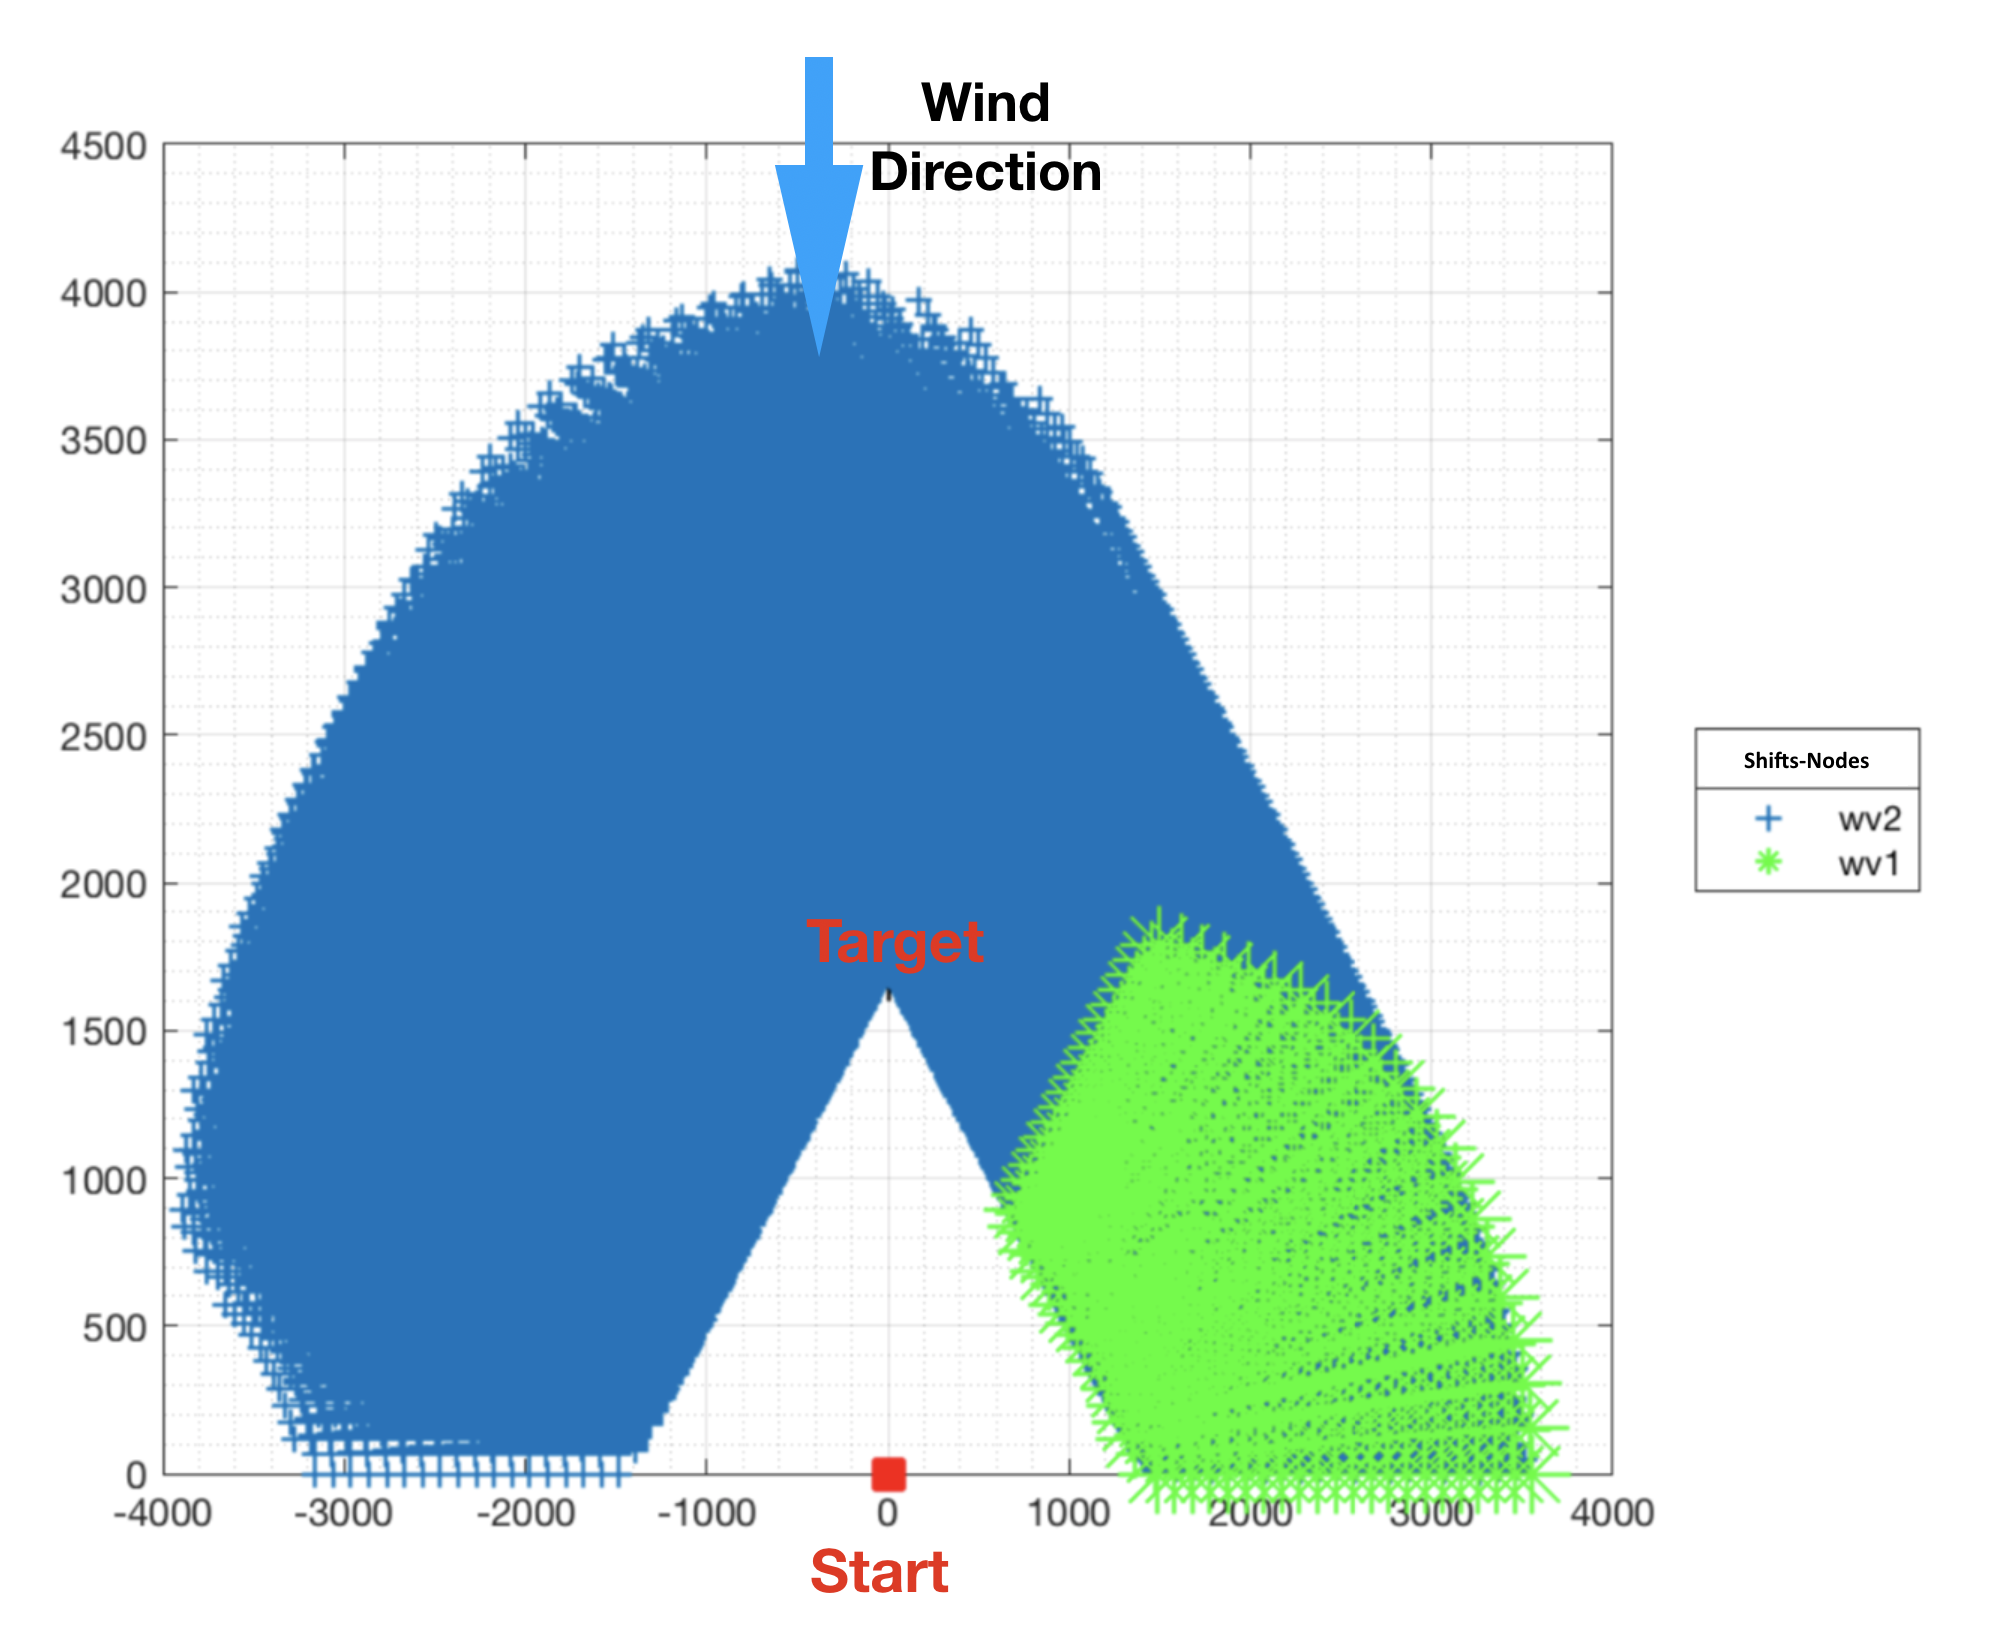
\includegraphics[width=0.45 \linewidth]{images/Nodes_2wv_5deg_5s.png}
    \caption{Nodes generated between 2 marks with one stage \textit{(n=1)} and  $\Delta \Psi = 5 \degree$}
    \label{fig:Onestages_NoGoZone}
\end{figure}

The values for the parameters and conditions to validate the algorithm are shown below. In this case, only half of the angles from the \acrshort{vpp}([0,$\pi$]) was used since it is assumed that it is symmetrical. Moreover, it is assumed constant wind conditions so the paths on both sides from the vertical line on the start mark are symmetrical. These parameter are:
\begin{itemize}
    \item \acrshort{v_tw}= 8.5 kn equivalent to 4.37 $ m/s $.
    \item \acrshort{b_tw}= 0\degree  from \textit{North}. 
    \item The distance between the start line and the next mark is \textit{0.977 nm} equivalent to 1809 meters. %\textit{0.96 nm} equivalent to 1730 meters. %1852 meters.
    \item The number of points stages is two, \textit{(n=2)}.
    \item The time step ($\Delta t$) is 5 seconds.
    \item The heading step angle ($\Delta \Psi$) is 1\degree. %5\degree.
    \item The $t_{tack-loss}$ = 10 seconds.
    \item The tolerance factor for the leg area are for $x_{SAtol}=2.5$ and for $y_{SAtol}=2$.
\end{itemize}

%For the next trial, $\Delta \Psi$ parameter was changed from 5\degree  to 1\degree, and the distance between marks was increased to \textit{0.977 nm} equivalent to 1809 meters, the rest of the parameter remains the same and only one side of the \acrshort{vpp} .
Under these condition more nodes were generated comparing with figure \ref{fig:Onestages_NoGoZone}, and in consequence more paths with even the same time. This is shown on figure \ref{fig:Paths_2wv_1deg_5s} where paths inside the same time range were plotted with the same color. The figure also shows that the fastest paths do not shift after 1200 meter from start point. In fact, figure \ref{fig:PathsTops_2wv_1deg_5s} shows that the paths with the top 5 times shifts before an horizontal distance of 1000 meters, which is only 10.5\% more than the mid-point distance between the marks. Despite the number of paths and its times the target mark hasn't reach perfectly 
%In this case with a smaller $\Delta \Psi$ and a larger distance between marks the paths never reach the target,
this is shown in figure \ref{fig:PathsZoom_2wv_1deg_5s}, where the second best time is the closets path within a radius of 6 meters from the target mark. % and it is the second best time that has this condition. \par
\begin{figure} [hbt!]
  \centering
  \subfloat[Paths generated with \textit{n=1} and $\Delta \Psi =1\degree$.] {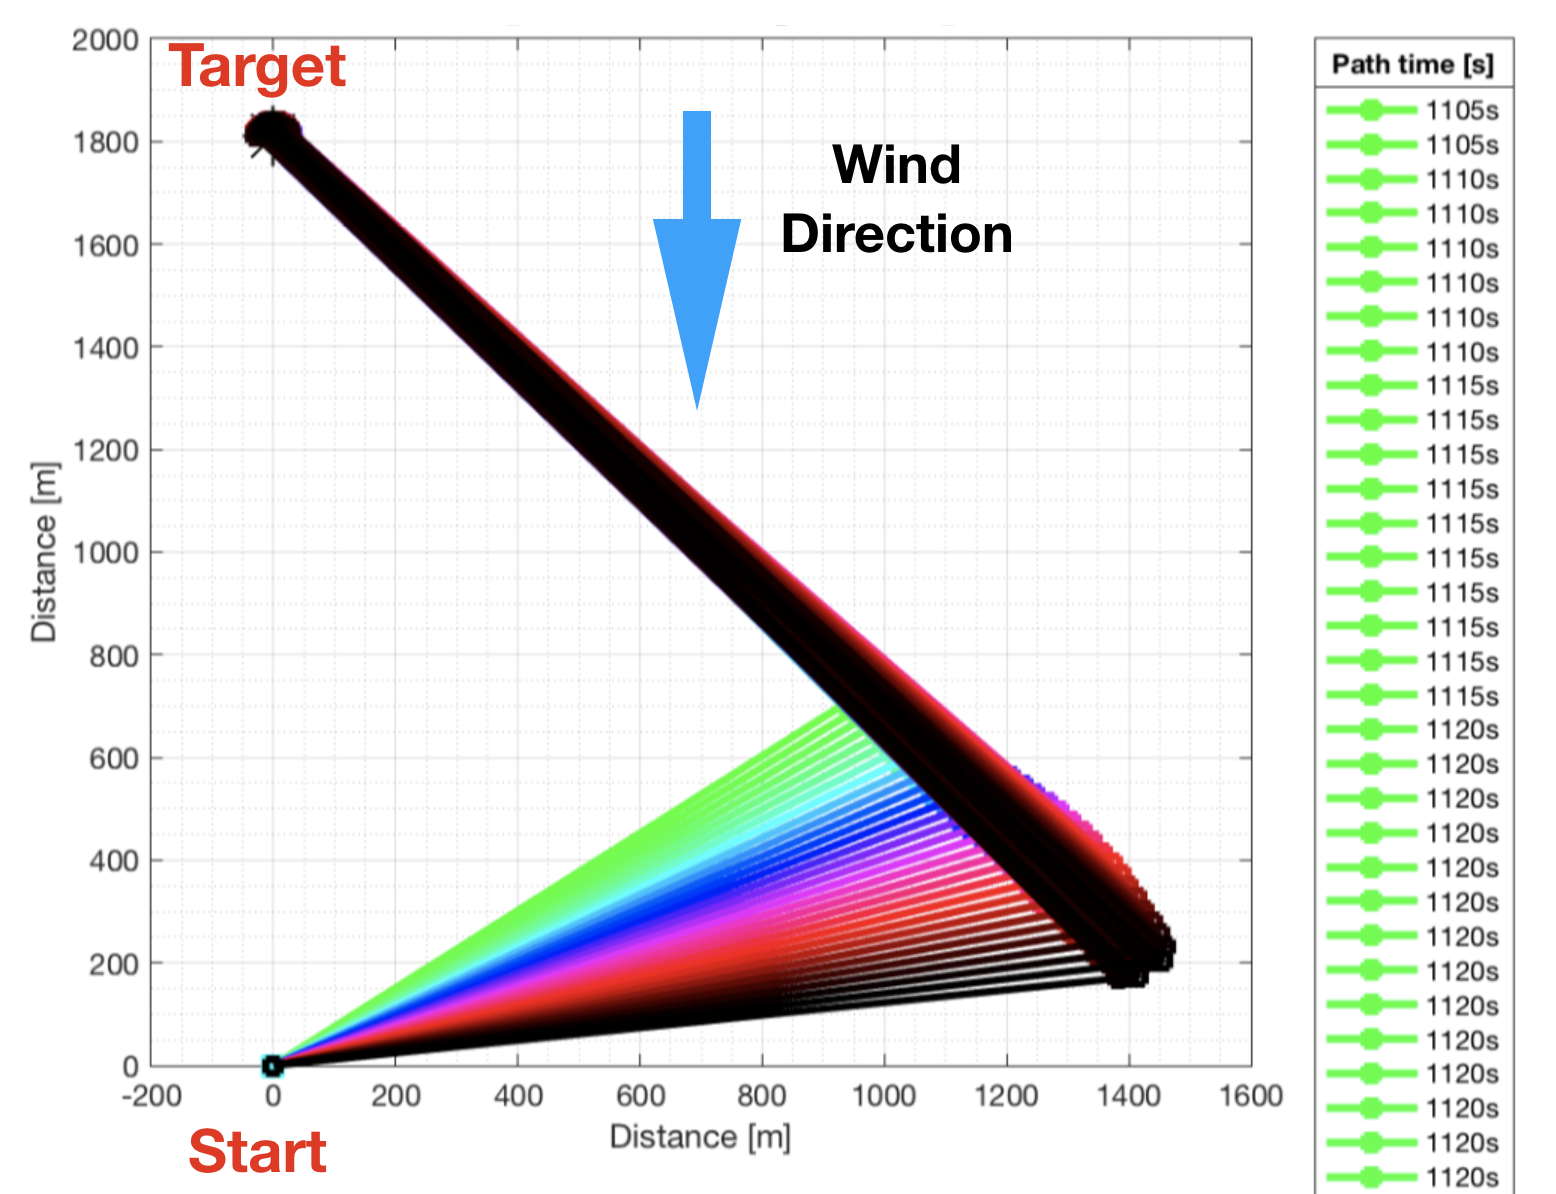
\includegraphics[width=0.31 \linewidth] {images/Paths_2wv_1deg_5s.png} \label{fig:Paths_2wv_1deg_5s}}
  \hfill
  \subfloat[Top 5 time paths and closets to the marked. These paths have the same time.] {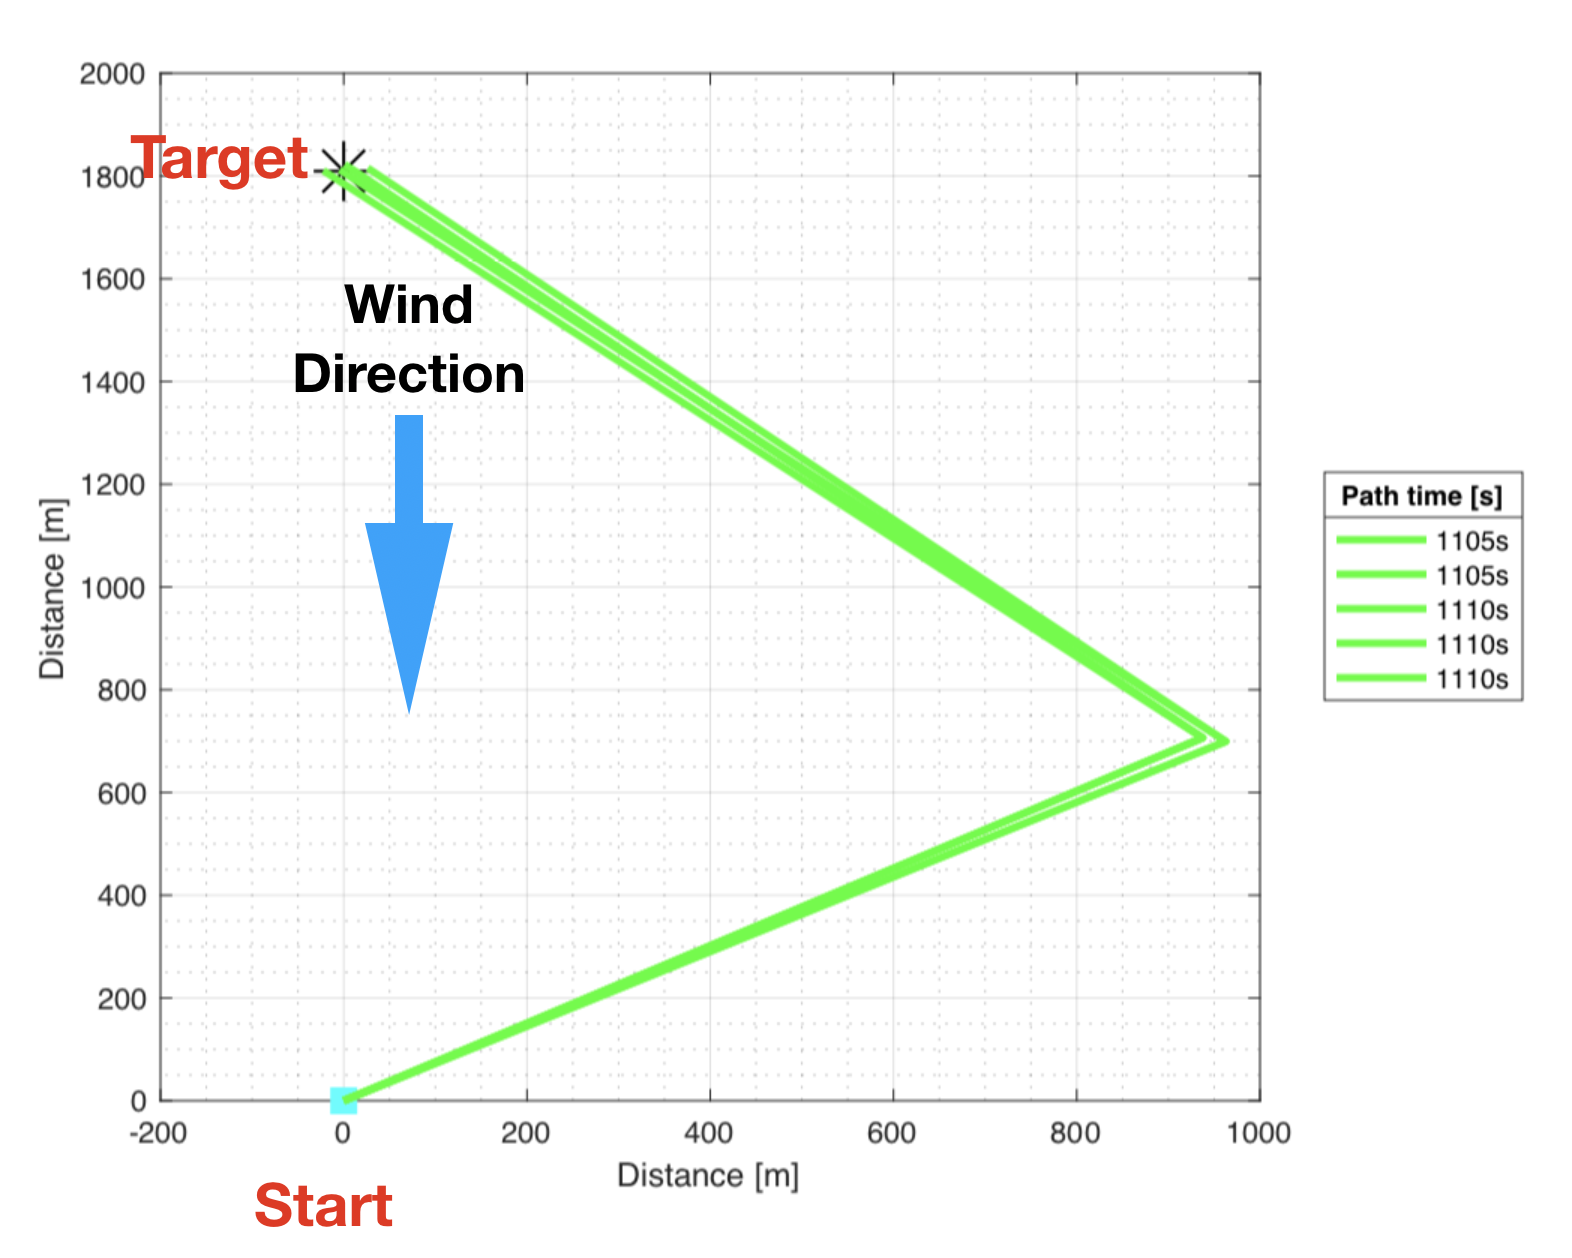
\includegraphics[width=0.31\linewidth]{images/PathsTop_2wv_1deg_5s.png}\label{fig:PathsTops_2wv_1deg_5s}}
  \hfill 
  \subfloat[Minimal time paths close-in end at the target mark.] {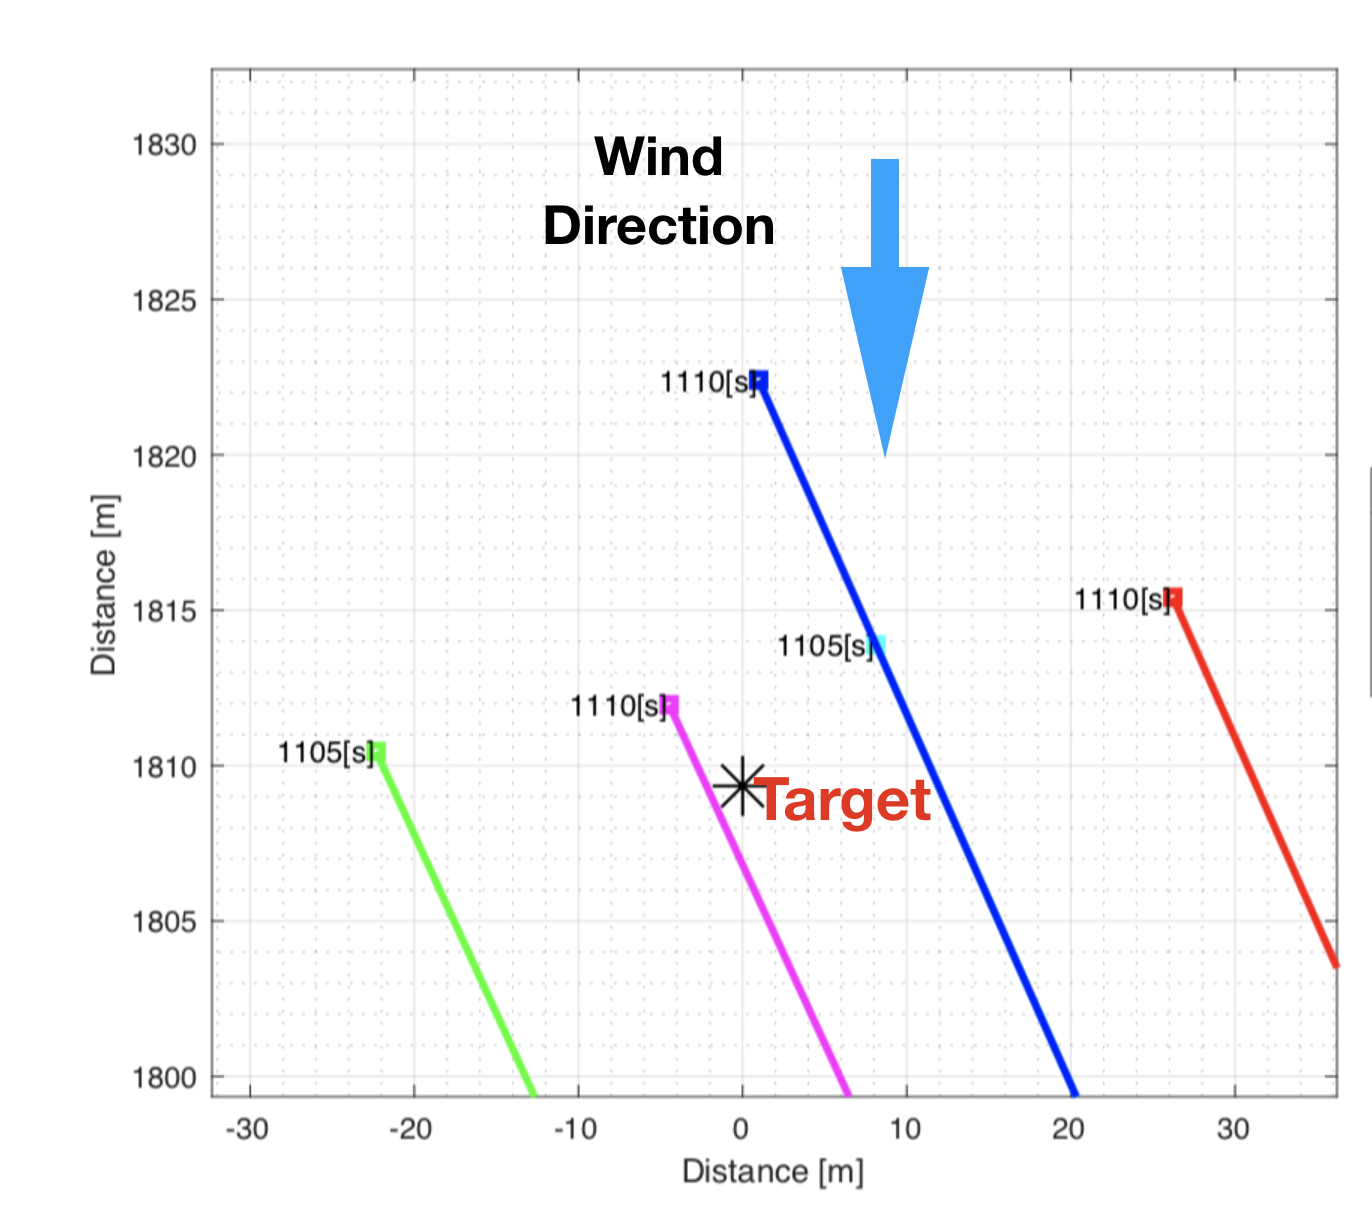
\includegraphics[width=0.31\linewidth] {images/ZoomPaths_2wv_1deg_5s.png} \label{fig:PathsZoom_2wv_1deg_5s}}
  \caption{Paths generated with one shift point in direction (\textit{n=1}) and $\Delta \Psi =1\degree$.}
\label{fig:Nodes_Paths_2wv_1deg_5s}
\end{figure}

When the number of point-stages increase to two (\textit{n=2}), not only the number of nodes and paths increase but the top 5 times also increase by 5 seconds. In this case the first shift in direction occurs at an horizontal distance form the start mark of 1100 meters and following the same heading-angle, figure \ref{fig:Path_3wv_1deg_5s}. The second shift on direction occurs within a radius of 46 meters from the target mark as show in figure \ref{fig:PathZoom_3wv_1deg_5s}. But despite all these alternatives the end of each of the paths does not reach perfectly the target mark. Figure \ref{fig:PathTops_3wv_1deg_5s} shows that all the paths with the same time ends within a radius of 3 meter from the target mark.  \par 

\begin{figure} [hbt!]
  \centering
  \subfloat[Top 5 times using 2 attacks with $\Delta t$ =5s and $\Delta \Psi =1\degree$. All paths have the same time of 1100s] {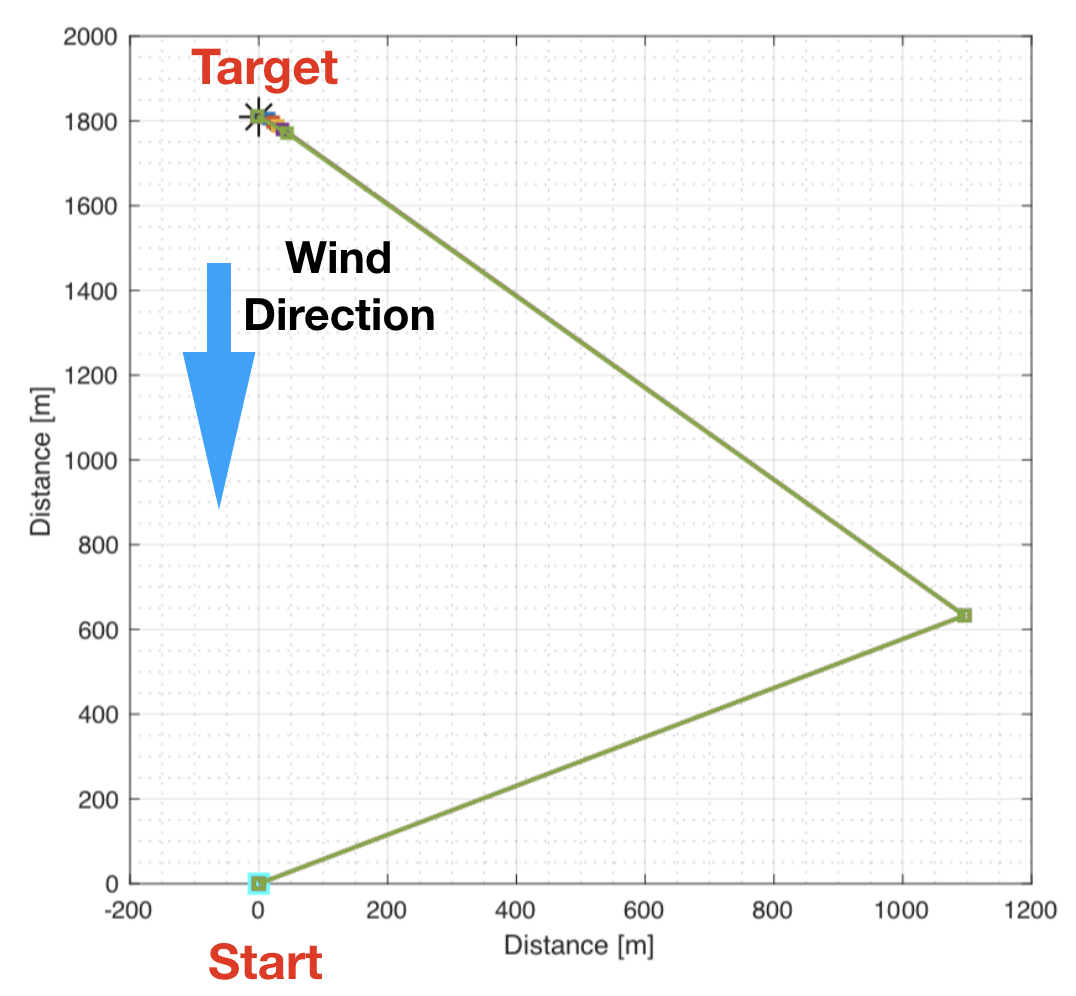
\includegraphics[width=0.31 \linewidth]{images/Paths_3wv_1deg_5s.png} \label{fig:Path_3wv_1deg_5s}}
  \hfill
  \subfloat[Close-up of the top 5 times at the target mark. The ends of paths are within a radius of 3m from the target mark.] {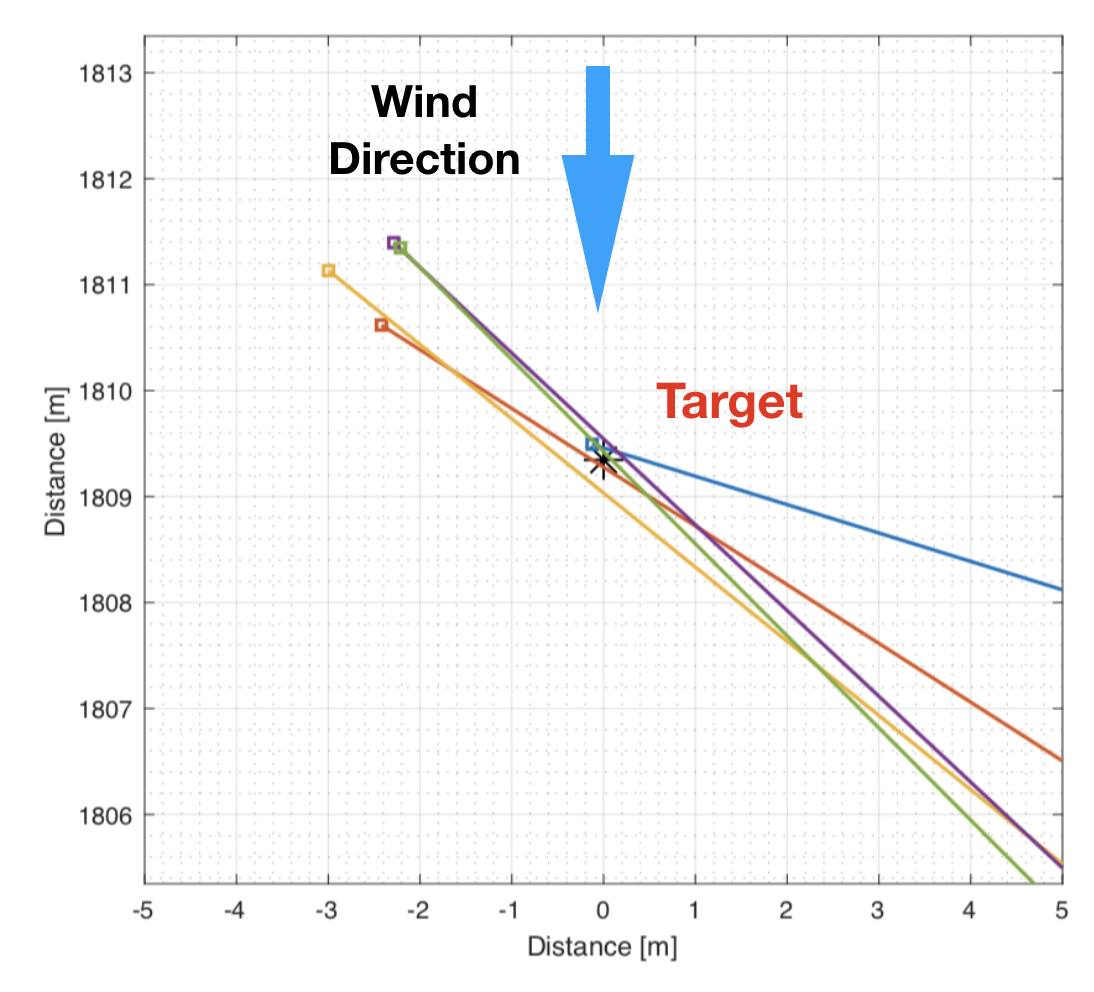
\includegraphics[width=0.31\linewidth]{images/PathsZoom_3wv_1deg_5s.png}\label{fig:PathTops_3wv_1deg_5s}}
  \hfill 
  \subfloat[Details about the shifts on direction after the first heading-direction was taken.] {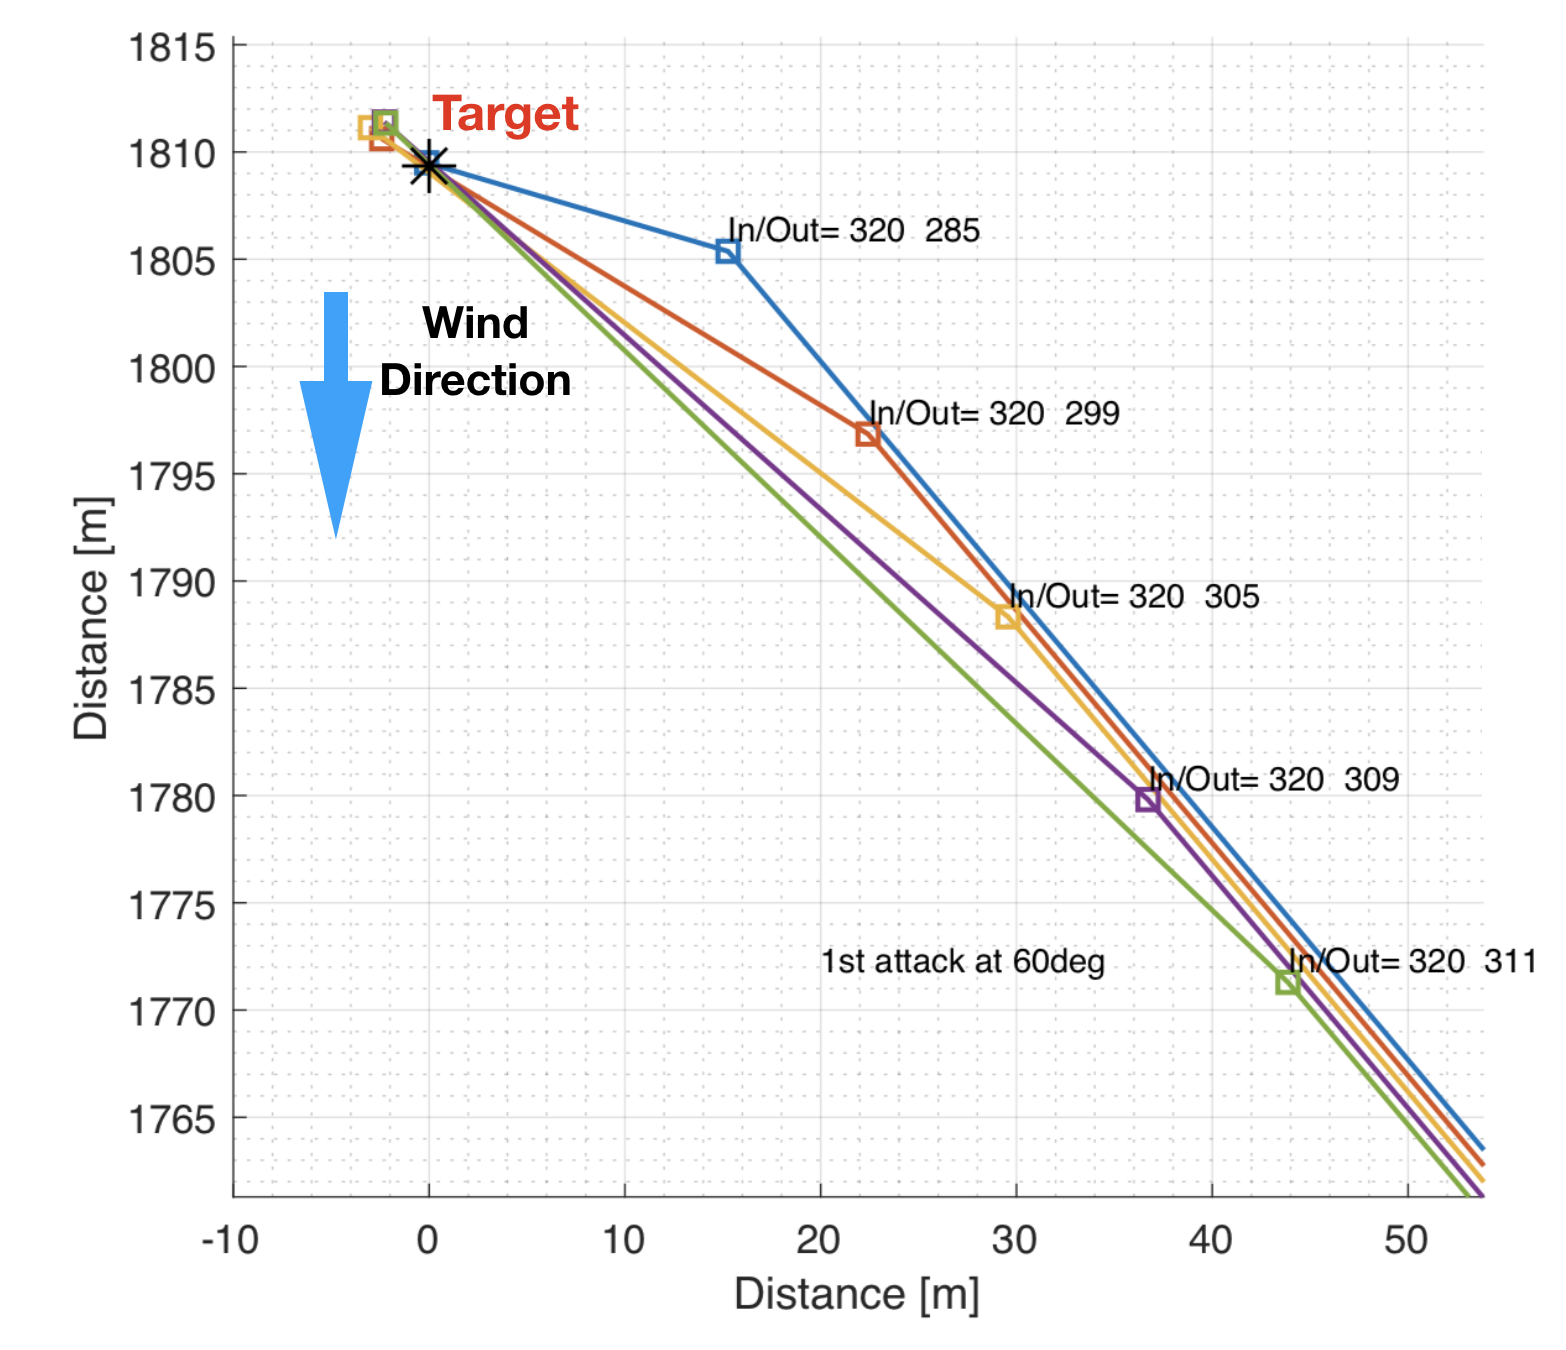
\includegraphics[width=0.31\linewidth] {images/PathsZP_3wv_1deg_5s.png} \label{fig:PathZoom_3wv_1deg_5s}}
  \caption{Top 5 time paths generated with two shift point in direction (\textit{n=2}) and $\Delta \Psi =1\degree$, the time of all them is 1100 seconds.}
  %Top 5 time paths and close-up at the target zone with two shifts in direction with $\Delta \Psi =1\degree$, } %$\Delta t$ =5s and
\label{fig:Paths_3wv_1deg_5s}
\end{figure}

From the previous results, it was clear that either another constrain or other type of adjustments to the algorithm are required to eliminates this kind of solutions. One of this changes refers to the definition of \textit{n}, which is the number of points inside each leg in order to define the number of internal stages within it. To represent this \textit{n} is a point with coordinates \textit{[X,Y]} inside a vector where its first set of values represent the coordinates of the star buoy and the last element are the coordinates of the end buoy. This means that \textit{n} are the number of points inside a vector and regardless the coordinates of these points they are linked to the legs using the buoys. It can be said that \textit{n} defines the size of a vector for the stage-state variables as in equation \ref{eq:n_vector}. \par
\begin{equation} \label{eq:n_vector}
\textrm{stage-state vector} = 
    \begin{bmatrix}
        x_{bouy,start} & y_{bouy,start} \\ 
        x_{1} & y_{1} \\
        \vdots & \vdots\\
        x_{n} & y_{n} \\
        x_{bouy,end} & y_{bouy,end} 
    \end{bmatrix}
\end{equation}

The value of \textit{n} stage points in this research is assigned to be \textit{7}, this means that inside each leg there are 8 stages where a shift in direction could occurs. Besides, at least 70 seconds could be added to the time's path if these shifts occurs along each leg. The locations of these \textit{n} is determined by the space constraints assigned to each leg and by the angle constraints, in other words by equations \ref{eq:Xmin_SailArea} to \ref{eq:Ymax_SailArea}. \par 

\begin{figure}[hbt!]
    \centering
    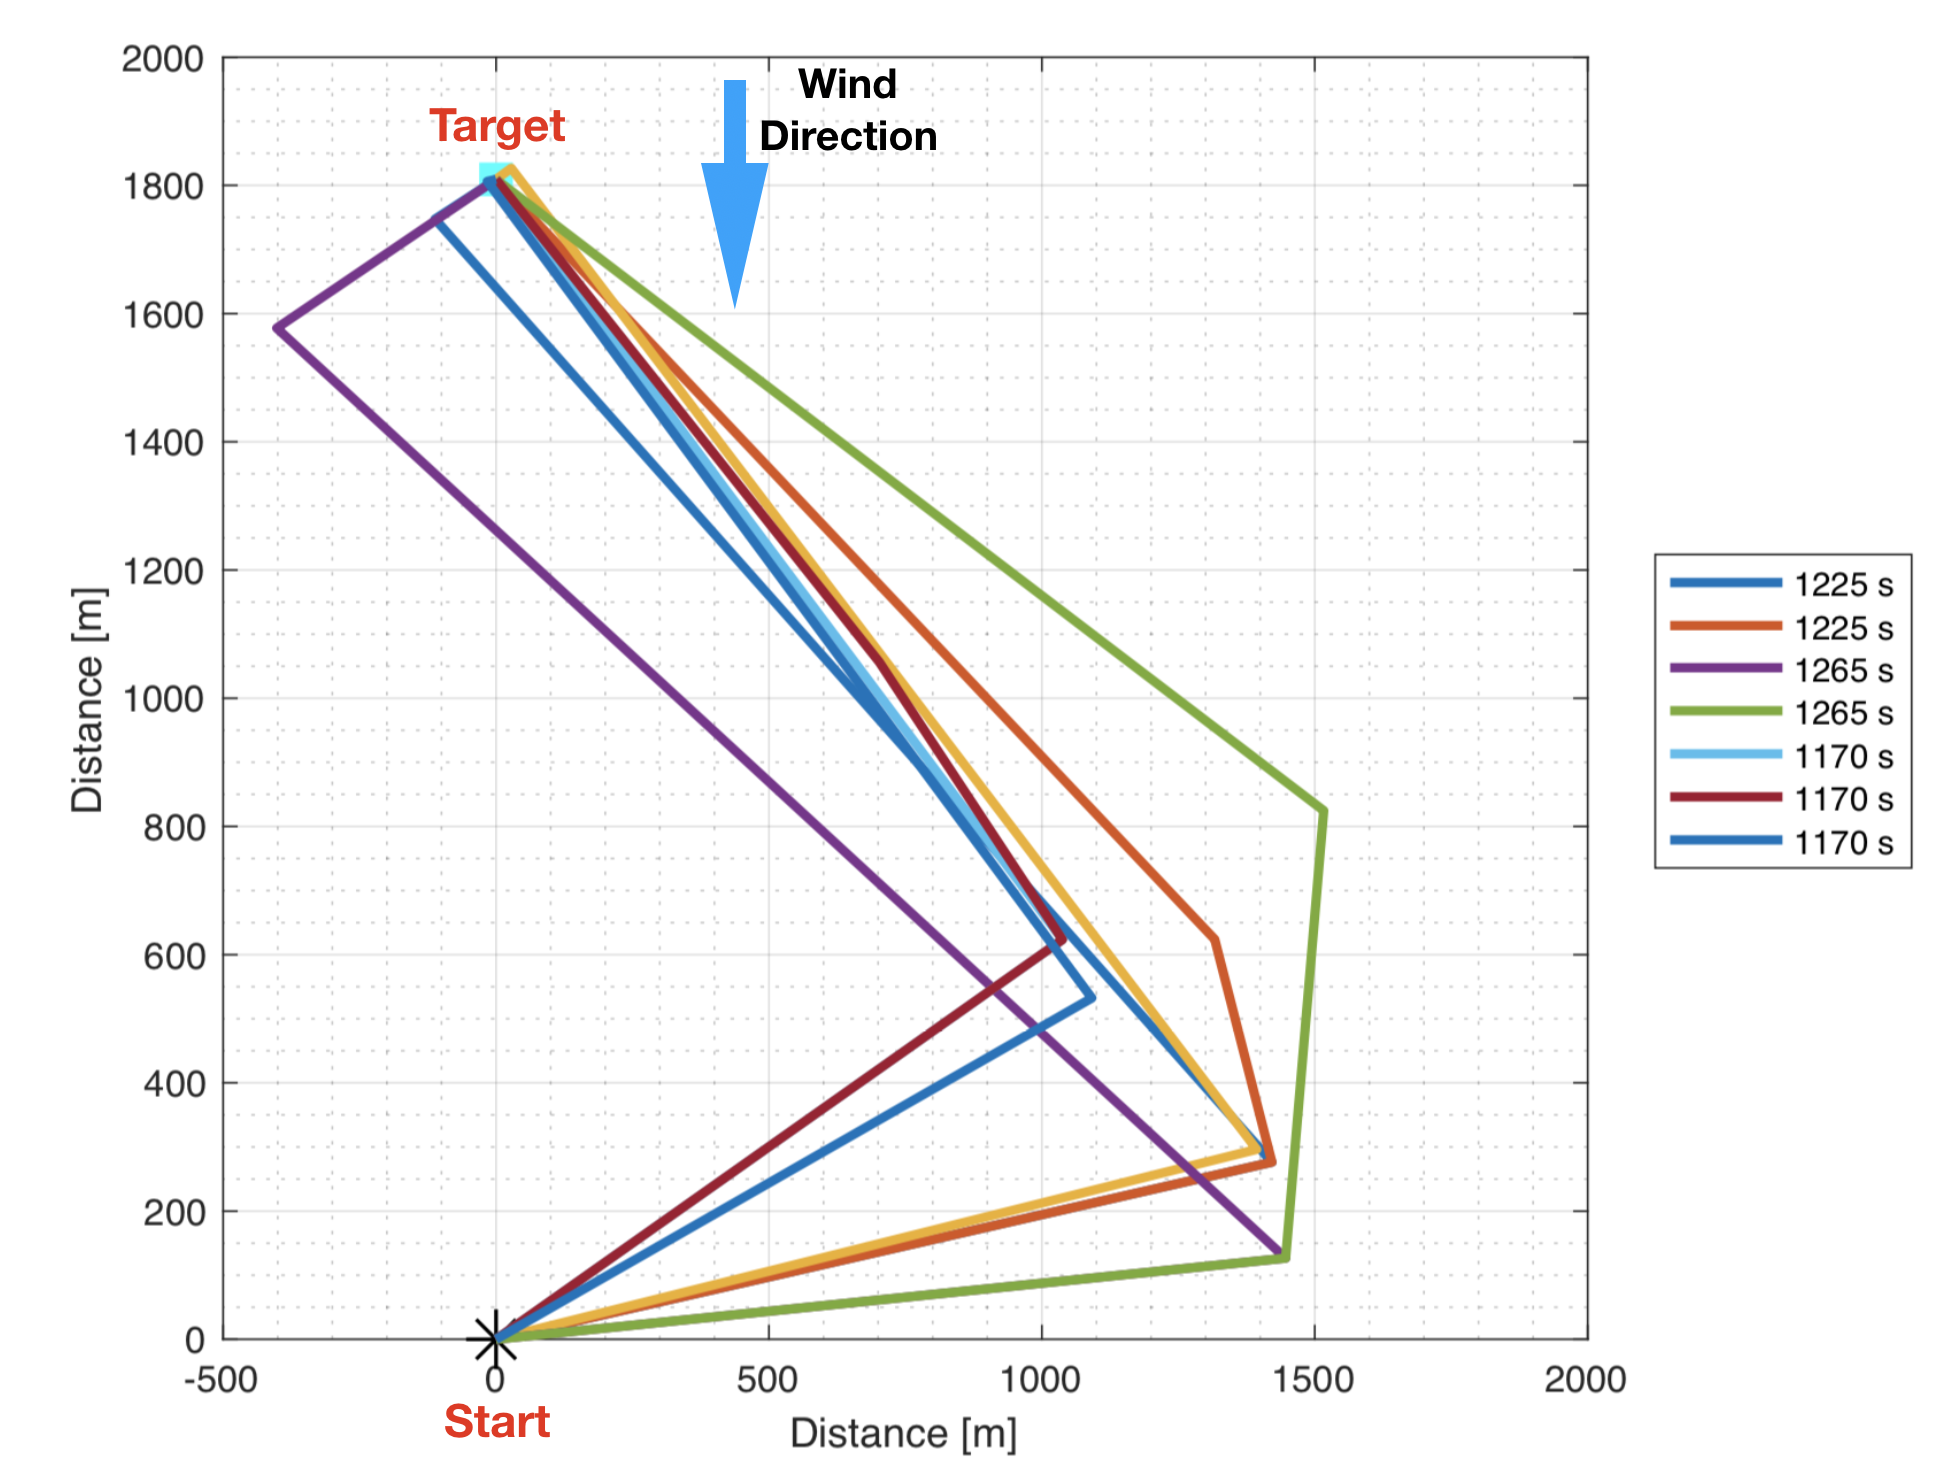
\includegraphics[width=0.45 \linewidth]{sections/n_stage_state_v.png}
    \caption{Paths generated using the stage-state vector \textit{n=2} and $\Delta \Psi =1\degree$}
    \label{fig:n_stage_state_vector_paths}
\end{figure}
Applying this changes figure \ref{fig:n_stage_state_vector_paths} shows some of the paths developed with them. It also shows that the fastest paths make the first shift before 1050 meters at an horizontal distance from the start mark. Furthermore, this distance is 1.15 times the mid-point distance between marks and this ratio is the same when \textit{n=2}, and equations equations \ref{eq:Xmin_SailArea} to \ref{eq:Ymax_SailArea}, use a factor ($x_{SAtol}$ and  $y_{SAtol}$) to scale up the area for each leg. Using these trials  %the maximum coordinate between the two buoys is required. 
equation \ref{eq:SailAreaTol} indicates the value of these tolerance factors, for now it is assumed that the value for each factor is the same for both coordinates. \par

\begin{equation} \label{eq:SailAreaTol}
    x_{SAtol}=y_{SAtol}=1.15
\end{equation}

Applying all thee changes the algorithm can developed paths that meet the constraints and estimate its time. For the optimization problem, particularly for the \textit{fmincon} function, where the option for the internal algorithm has to set as \textit{'active-set'}. This option allows the algorithm to take large steps far from the target so the number of iterations and evaluations of the algorithm are used effectively to find the optimal solution. It was observed that without this change, the solution takes a larger number of iterations and evaluations of the function to get the optimal solution. Besides, most of the time this solution is not even the optimal compared with the solutions provided with the \textit{'active-set'} method. \par 

After making these changes in the algorithm and adding trapezoidal route as figure \ref{fig:Rio_Course1}, with the same \acrshort{v_tw} as previously defining but with \acrshort{b_tw} about 140\degree. The optimal path for the race is shown in figure \ref{fig:Val_route}, where each leg is indicated by a different color, the total time is about 56 minutes. Because the wind is constant in time and space the fastest trajectory in a downwind and direct wind is by following a straight line. \par \noindent 
The optimal path for the upwind mode on leg 1 was found by developing 2 routes where the start conditions meet the constraints.  These two conditions where optimized using the algorithm and the minimal time between them provides the optimal path for the leg. Figure \ref{fig:Val_leg1} shows these 4 paths, the path marked in green was used to construct the optimal path for the race and it was used as a constraint for the second leg. \par 

\begin{figure} [hbt!]
  \centering
  \subfloat[Leg 1, Upwind Mode ] {\includegraphics[width=0.4 \linewidth]{sections/Val_leg1.png} \label{fig:Val_leg1}}
  \hfill
  \subfloat[Race Optimal Path per leg] {\includegraphics[width=0.525\linewidth]{sections/Val_route.png} \label{fig:Val_route}}

  \caption{Validation} %$\Delta t$ =5s and
\label{fig:Val_algorithm_Route}
\end{figure}

The optimal time path or the minimal time path can be found by finding the minimal times per leg, the initialization of the algorithm requires initial guess for the variables used. Because the system is non-linear due to the no-convex shape of the \acrshort{vpp} the optimal solution is not unique. The algorithm developed considers two initial guess values for the variables, after the optimization is done the results are compared to find the minimal time path between them.  
The algorithm uses the heading-direction approach to find the optimal path, and it divides each leg on stages. \par 
\noindent
These points also controls and limits the number of shifts in direction that define the zig-zag pattern specifically in the upwind mode. % These shifts are particularly common on the upwind mode. 
Furthermore, the points-stages \textit{(n)} inside the leg enable the continuity between legs, this continuity is constrained by the angle between legs and between these points. The locations of these points are limit by the area assigned to each leg, since the space area determine the number of nodes or coordinates where these points can be located. Most important, the area must be contained inside wind model area and it has to be large enough to estimate the wind's velocity (\acrshort{v_tw}) and direction (\acrshort{b_tw}) at any time and location. 
%since a tight area limits the number of datasets available to estimate the wind's velocity (\acrshort{v_tw}) and direction (\acrshort{b_tw}) at any time and location. 
\par Now that the algorithm was validated to developed paths, estimate its time and optimized them to get the minimal time path the next chapter will evaluate 2 conditions for the time-step. 





%at 0\degree (\acrshort{b_tw})  while the distance between the start line and the next buoy is \textit{1 nm} equivalent to 1852 meters and with different valuetimes for the stages. The first condition to test is with only one stage (\textit{n=1}), 


%First to review if the algorithm can make attacks when the wind mode to sail is \textit{upwind} and if the es
%\section{Considerations: Results from  the Validation}
%During the \textit{upwind} wind mode the sailboat is prone to follow a zig-zag pattern 
%Because of this, the wind properties are setup

%[x,y] = mfwdtran(lat,lon)
%\subsection{Wind Model}
%Weather model forecast are calculated  by super computer and updated every three hour according regions. Different agencies have developed models to predict it in global terms. The local prediction are made based on it with via extrapolation and interpolation between local measurements with the intention to predict it every hour, for local purposes. The global and open information is stored in what is know as GRIB or NET files. This files, GRIB, is downloaded according the region of interest the common grid size provides is a 3 km square. 
%In \cite{binns2002development} the simulator use a guts wind model  with the next parameters: the time step was defined as 60 seconds and the length of 200 m. It can be said that the grid 

%definition of the wind area and its implementation into the sail course 

%\begin{figure} [hbt!]
 %   \centering
  %  \includegraphics[width=0.5 \linewidth ]{windArea.png}
  %  \caption{Wind Area Concept using a wind model representation. The lines in red are the ctr and limits of the sail area, which can be inscribed on a square.}
   % \label{fig:WindAreaSketchLEG}
%\end{figure}
\chapter{Simulations: Time and Trajectory using the optimizer algorithm}

\section{Software Parameters and others set-up}
\section{The Scenarios to Simulate the Minimal Time Path}
\subsection{Constant Wind, Time Step of 1 Hour}
\subsection{Constant Wind, Time Step of 10 Minutes (1/6 Hour)}
\subsection {Wind data measured during competition}

\chapter{Conclusions and Recommendations}


\bibliographystyle{unsrt} %ieeetr %alpha %apalike unsrt
\bibliography{sections/thesisref}
\addcontentsline{toc}{chapter}{Bibliography}

\listoffigures
\addcontentsline{toc}{chapter}{List of Figures}
\listoftables
\addcontentsline{toc}{chapter}{List of Tables}

\printglossary[type=\acronymtype]
\addcontentsline{toc}{chapter}{List of Acronyms}

\end{document}